%
% Chapter 4
%
% multiPANTS

\chapter{multiPANTS: response to biologic anti-TNF therapy for CD}

% Collab note
% - PANTS collab
% - RNAseq gen and quant
% - Cell count estimates

\begin{outline}

\section{Introduction}

\subsection{\Glsfmtlong{CD}}

% \1 <Description>
\1 CD is a chronic inflammatory disease of the gastrointestinal tract.
    \2 CD is one of the two forms of IBD, characterised by patchy inflammation, where lesions are interspersed with regions of normal mucosa. The lesions can be distributed anywhere in the gastrointestinal tract, and tend to be transmural, affecting all layers of the gut wall.
    \2 The second form, UC is characterised by continuous inflammation, with lesions that are superficial rather than transmural, and restricted to the colon. \autocite{roda2020CrohnDisease}
    \2 Although these are two distinct forms of IBD, similarities in symptoms, therapies, genetic architecture mean they have historically been studied together.
        \3 The similarity is such that there is a subset of IBD-U patients with features of both CD and UC, and thus is difficult to classify as one or the other.
    \2 CD and UC are considered IMIDs, a group of related conditions involving immune dysregulation of common inflammatory pathways.
        \3 Other diseases include type 1 diabetes (T1D), systemic lupus erythematosus (SLE), rheumatoid arthritis (RA), multiple sclerosis (MS) and psoriasis. \autocite{cotsapas2013ImmunemediatedDiseaseGenetics,david2018GeneticsImmunemediatedInflammatory}

% \1 <Pathogenesis and host genetics>
\1 Pathogenesis of CD is not completely understood, but involves interaction of the immune system, environmental factors (e.g. smoking, stress, diet \autocite{ananthakrishnan2015EpidemiologyRiskFactors,roda2020CrohnDisease}), and gut microbial factors in a genetically-susceptible individual \autocite{desouza2016ImmunopathogenesisIBDCurrent}.
    \2 Since the seminal discovery of association of \gene{NOD2} with CD in 2001 \url{https://www.nature.com/articles/35079223} (the first gene to be genetically-associated with a common disease), and the first IBD GWAS in 2006 \url{https://www.ncbi.nlm.nih.gov/pmc/articles/PMC4410764/}, a lot of progress has been made in establishing genetic risk factors.
    \2 The most recent GWAS studies define over 240 risk loci for IBD \autocite{delange2017GenomewideAssociationStudy}
    % \2 IBD GWAS identify loci that are in pathways that are drug targets \autocite{delange2017GenomewideAssociationStudy}
    \2 Genetic correlation between UC and CD is high \autocite{cotsapas2013ImmunemediatedDiseaseGenetics,david2018GeneticsImmunemediatedInflammatory}
    \2 Most GWAS hits are shared, but there is some heterogenenity of effects between CD/UC, mostly notably at NOD2, which is much stronger for CD \autocite{jostins2012HostMicrobeInteractions,liu2015AssociationAnalysesIdentify}
    \todo{add NOD2 OR}
    \2 Concordance rates amongst monozygotic twins are higher for CD (~50\%) than for UC (\textapprox{15}\%) suggesting a greater heritable component \autocite{roda2020CrohnDisease}

% \1 <Epidemiology and burden>
\1 IBD has historically been considered a disease of the Western world.
    \2 The disease burden is now rising globally \autocite{kaplan2015GlobalBurdenIBD,alatab2020GlobalRegionalNational}.
    \2 The highest prevalence and incidence of new cases of CD are in North America and western Europe. \autocite{roda2020CrohnDisease}
    \2 CD is becoming increasingly common in newly industrialized countries in Asia, Africa and South America.
        \3 Migrants from low- to high- prevelance regions are at higher CD risk, suggesting there is an influence of Western lifestyle on disease risk. \autocite{roda2020CrohnDisease}
    \2 The modal age of onset of CD is typically between late adolescence and early adulthood.
    \2 CD is progressive: Within 20 years of diagnosis, 50\% of patients with CD develop gastrointestinal tract complications and approximately 15\% require surgical intervention \autocite{roda2020CrohnDisease}
    \2 Given the rising prevelance and large impact on quality of life, there is active research into effective therapies that lead toward the end goal of complete mucosal healing \autocite{levin2016MechanismActionAntiTNF,roda2020CrohnDisease} 

\subsection{Anti-TNF biologic therapies for CD}
\todo{as suggested, the subsection on anti-TNFs in the intro chapter will likely be merged here}

\1 \gls{TNF} (sometimes referred to by it's archaic name \gls{TNF}-\textalpha), is a proinflammatory cytokine
    \2 It is synthesised mainly by immune cells: macrophages, NK, T and B cells in transmembrane form, then cleaved into the soluble form.
    \2 Binding of \gls{TNF} to either of its two downstream receptors (most cells in the body express one or the other) on immune and gut mucosal cells triggers a signalling cascade that in different contexts, can regulate inflammation, apoptosis, cell proliferation and survival. \autocite{aggarwal2003SignallingPathwaysTNF,kalliolias2016TNFBiologyPathogenic,digby-bell2019InterrogatingHostImmunity}
    \2 In the IBD pathogenesis context, TNF mediates gut inflammation. One current model is TNF promoting gut epithelial apoptosis; and inhibiting T cell apoptosis, which maintains chronic inflammation. \autocite{levin2016MechanismActionAntiTNF,adegbola2018AntiTNFTherapyCrohn,digby-bell2019InterrogatingHostImmunity}
        % \3 T cell macrophage interaction: apoptosis, regulation, inhibition of proliferation TODO

\1 The use of anti-gls{TNF} therapy has revolutionised CD and IBD patient care in the last two decades.
    \2 The two major agents used are adalimumab and infliximab. Both are IgG1 monoclonal antibodies that binding to both soluble and transmembrane TNF, inhibiting interaction with it's receptors \autocite{lichtenstein2013ComprehensiveReviewAntitumor,adegbola2018AntiTNFTherapyCrohn}
    \2 two major mechanisms of anti-TNFs: have been proposed induction of T cell apoptosis in the gut mucosa, and Fc dependent mechanism inducing wound-healing M2 macrophages \autocite{levin2016MechanismActionAntiTNF}
        \3 Fc regions fixing complement can also lyse cells expressing membrane TNF \autocite{adegbola2018AntiTNFTherapyCrohn}
    % \2 leads to drop in circulating markers like CRP \autocite{levin2016MechanismActionAntiTNF}
    \2 adalimumab is a human monoclonal antibody
        \3 typically administered subcutaneously (via auto-injector pen) every two weeks, after 2 dose induction \autocite{adegbola2018AntiTNFTherapyCrohn}
    \2 infliximab is a chimeric (mouse/human)
        \3 taken via intravenous infusion, typically on a maintenance schedule of every eight weeks after an initial three-dose induction \autocite{adegbola2018AntiTNFTherapyCrohn}
        \3 more immunogenic (more anti-drug antibodies that interfere with drug activity), thought to lead treatment failure via lowering drug concentrations \autocite{kennedy2019PredictorsAntiTNFTreatment} \url{https://journals.sagepub.com/doi/10.1177/1756283X17750355}
    % \todo{I assume dosing follows the induction and maintenance schedule from \autocite{adegbola2018AntiTNFTherapyCrohn}. Can't find anything about it in the PANTS protocol, although Sim confirmed the 2w/8w frequencies.}
    \2 ADA and IFX together are very costly: 29B USD in 2017 "the-global-use-of-medicine-in-2019-and-outlook-to-2023.pdf"
\1 What determines which drug is given?
    \2 e.g. guidelines:
        \3 2010 ECCO: "all currently available anti-TNF therapies appear to have similar efficacy and adverse-event profiles, so the choice depends on availability, route of delivery, patient preference, cost and national guidance.” \url{https://www.nature.com/articles/nrgastro.2015.135}, also see "Figure 2: Biologic agents in IBD: a proposed algorithm for clinical practice."
        \3 \autocite{dhaens2011LondonPositionStatement}
        \3 2018 <Infliximab and adalimumab for the treatment of Crohn's disease> \url{https://www.nice.org.uk/guidance/ta187}>
        \3 2019 <British Society of Gastroenterology consensus guidelines on the management of inflammatory bowel disease in adults \url{https://gut.bmj.com/content/68/Suppl_3/s1.full}>
    \2 It is currently not able to predict efficacy. Treatment failure is not uncommon.

\subsection{Treatment failure}

\1 There many types of failure: \gls{PNR} within the induction period (12-14 weeks for ADA/IFX), secondary non-response, non-remission, adverse events \url{https://journals.lww.com/ctg/Fulltext/2016/01000/Loss_of_Response_to_Anti_TNFs__Definition,.2.aspx}
    \2 e.g. failure rate estimates
        \3 "The incidence of PNR varies between clinical trial and clinical practice from 10–20\% to 13–30\%.2, 3, 5" 2013 \url{https://pubmed.ncbi.nlm.nih.gov/23792214/}
        \3 "nonresponse for TNF antagonist therapy varies between clinical trial and clinical practice from 10 to 30\%,2–4 and the annual risk of secondary nonresponse from 13\% per patient year for infliximab (IFX)5 to 20.3\% for adalimumab.6" 2018 \url{https://www.ncbi.nlm.nih.gov/pmc/articles/PMC5784543/}
        \3 "Unfortunately, anti-TNF treatment failure is common: 10–40\% of patients do not respond to induction therapy (primary non-response),6–8 24–46\% of patients have secondary loss of response in the first year of treatment,9 and approximately 10\% have an adverse drug reaction that curtails treatment.10" \autocite{kennedy2019PredictorsAntiTNFTreatment}
    \2 also, immunogenicity leads to non-response via anti-drug Abs; serum drug levels correlated with efficacy, anti-drug Abs are inversely correlated \autocite{lichtenstein2013ComprehensiveReviewAntitumor}
    \2 although mucosal healing is the preferred gold standard \autocite{roda2020CrohnDisease}, could be argued that PNR is important, as it's correlated with remission, and measurable early for stratification

\1 when they fail: anti-TNFs biologics just one part of the therapy pyramid for CD \url{https://www.nature.com/articles/nrgastro.2013.158}
    \2 a pyramid with higher toxicity/patient impact and high cost at the top
    \2 Two approaches to treat patients, neither are ideal
        % adegbola2018AntiTNFTherapyCrohn
        % "Consensus guidelines recommend “step-up” treatment with initial trials of
        % immunosuppressive treatment (corticosteroid and steroid sparing immunomodulators) prior to
        % starting anti-TNF agents [8,9], although there is increasing evidence advocating for early institution
        % of anti-TNF treatment [10], the “top-down” approach, especially in severe disease phenotypes [11].
        % In this review, we focus on the use of anti-TNF therapy in Crohn’s disease, its mechanism of action,
        % role and future directions in therapeutic use."
        \3 Step-up approach: may undertreats patients that require more aggressive therapy, allowing disease time to progress
        \3 Top-down approach: exposes patients to risks from more aggressive therapies they may not need from overtreating
        \3 recent moves towards a hybrid: start at biologics and go top-down if possible \url{https://www.ncbi.nlm.nih.gov/pmc/articles/PMC5784543/}
        % \3 ECCO recommendations \url{https://academic.oup.com/ecco-jcc/article/11/7/769/2962457}
    \2 after failure of biologics, other options include dose intensification, and switching to an agent with diff mech \autocite{lichtenstein2013ComprehensiveReviewAntitumor}
    \2 But better still would be to target the right therapy to those that require and respond to it
    \2 baseline predictors would be especially valuable for patient stratification

\subsection{Predicting response to anti-TNFs for CD}

\1 previously reported clinical predictors include age, disease duration, BMI, smoking, CRP, FCP, anti-TNF drug and anti-drug antibody concentrations, but these have mostly been found in small retrospective cohorts, and rarely independently validated \autocite{dhaens2011LondonPositionStatement,ding2016SystematicReviewPredicting,kopylov2016PredictingDurableResponse,flamant2018InflammatoryBowelDisease,digby-bell2019InterrogatingHostImmunity,noor2020PersonalisedMedicineCrohn}
    \2 in PANTS: a recent prospective study of ADA and IFX for CD to date: large n=1610 \autocite{kennedy2019PredictorsAntiTNFTreatment}
    \2 PNR has observed at a 23.8\% rate, evaluated at w14 via clinical decision algorithm.
    \2 low serum drug concentration in peripheral blood at w14 (ELISA) was associated with PNR, and also non-remission and immunogenicity for both drugs
    \2 no associations at baseline

\1 Studies have also attempted to define transcriptomic predictors for anti-TNF response in IBD \autocite{digby-bell2019InterrogatingHostImmunity,noor2020PersonalisedMedicineCrohn}
    \2 gut:
    \2 \autocite{arijs2009MucosalGeneSignatures}: TNFRSF11B, STC1, PTGS2, IL13RA2 and IL11. endoscopic and histological healing. infliximab. UC. colon mucosal biopsy. total n 46.
    \2 \autocite{arijs2010PredictiveValueEpithelial}: (TNFAIP6, S100A8, IL11, G0S2, and S100A9). complete endoscopic and histologic healing. infliximab. Crohn's colitis CDc. gut biopsy. 19
    % \2 Halloran 2014 \url{https://www.ncbi.nlm.nih.gov/pmc/articles/PMC4985265/} "molecular disturbance" aka PC1 seems to sep R and NR in Pathogenesis-based transcript sets (PBTs)
    \2 \autocite{west2017OncostatinDrivesIntestinal}: OSM and OSM-hier cluster module.  multiparameter measures clinial Mayo score.  UC.  gut mucosal biopsy.  227.
    \2 GIMATS \autocite{martin2019SingleCellAnalysisCrohn}:
    expression of IgG plasma cells, inflammatory mononuclear phagocytes, activated T cells, and stromal cells, which we named the GIMATS module.  various anti-TNF therapy.  ileal CD.  achieving durable (6 months) corticosteroid-free clinical remission (pediatric Crohn’s disease index (PCDAI) < 10) at months 18 and 24 post-diagnosis, as responders.  inflamed ileal biopsies.  n=340 two cohorts with baseline.

\1 blood: prognostic tests performed on blood samples are non-invasive and hence of high value.
    \2 there is conflict in existing studies on TREM1
    \2 \autocite{gaujoux2019CellcentredMetaanalysisReveals} : endoscopic score and/or clinial decision algorithm.  infliximab. .
        \3 gut biopsy:   proportion of plasma cells.  following adjustment to plasma cells and activated monocytes from expression deconv, TREM1 is upstream reg of resulting DEGs: TREM-1 is expressed on myeloid lineage cells including monocytes and macrophages, has well-documented proinflammatory functions.  81 patients.
        \3 \autocite{gaujoux2019CellcentredMetaanalysisReveals}: TREM1 down in NR. blood.  endoscopic.  CD.  22 patients.
    \2 \autocite{verstockt2019LowTREM1Expression}: opposite. Baseline whole blood TREM1 was downregulated in future anti-TNF responders. endoscopic remission. ifx and ada. IBD.
    \2 difference may be due to sample size, ethnicity, definition of response \url{https://pubmed.ncbi.nlm.nih.gov/30007919/} \autocite{digby-bell2019InterrogatingHostImmunity}
    \2 \autocite{salvador-martin2020GeneSignaturesEarly} SMAD7, TLR2 and DEFA5. response based on decrease in Pediatric Crohn’s Disease Activity Index (PCDAI) and Pediatric Ulcerative Colitis Activity Index (PUCAI). pIBD, IFX/ADA. n=31

\1 Finally, genetic markers for non-response \autocite{flamant2018InflammatoryBowelDisease}
    \2 baseline by definition
    \2 anti-TNF response does not necessarily share the same genetic architecture as disease risk loci e.g. polymorphisms in IBD risk lock NOD2, TNFR1, TNFR2 are not associated with NR to infliximab \autocite{digby-bell2019InterrogatingHostImmunity,noor2020PersonalisedMedicineCrohn}
    \2 IL-13 receptor (IL13Rα2), IL-23 receptor (IL23R), TNF-receptor I (TNFRI), IgG Fc receptor IIIa (FcYRIIIa), neonatal Fc receptor (VNTR2/VNTR3), apoptosis-related genes (Fas ligands, caspase 9), and MAP kinases, FAS-L, caspase 9 \url{https://www.ncbi.nlm.nih.gov/pmc/articles/PMC6128143/} \autocite{flamant2018InflammatoryBowelDisease}, and also multi-SNP risk scores \url{https://www.ncbi.nlm.nih.gov/pmc/articles/PMC6128143/}
    \2 but like transcriptomic predictors, mostly small candidate gene studies
    % The HLA-DQA1*05 allele, carried by approximately 40% of Europeans,
    % significantly increased the rate of immunogenicity (hazard ratio [HR],
    % 1.90; 95% confidence interval [CI], 1.60–2.25; P ¼ 5.88  10–13).
    % Both drugs, and regardless of immunomodulator
    % Dominant effect
    \2 although no GWAS hits for PNR in PANTS, a related phenotype, immunogenicity is associated with HLA-DQA1*05 \autocite{sazonovs2019HLADQA105Carriage}, so there may be some promise in the area

\1 in summary, varying in technology used to measure gene expression, analysis method, anti-TNF drug, response definition (both criteria and time of assessment), tissue, sample size, disease among all these studies make a consensus hard to establish.
    \2 none of these clinical, transcriptomic, or genetic markers have been sufficiently discriminative and validated for use predicting NR in the clinic yet, although several are undergoing validation \autocite{noor2020PersonalisedMedicineCrohn}

\subsection{Chapter summary}

\todo{this subsection}
\1 <context>: summary of above
    \2 conflicting results in the literature and need for validation for transcriptomic signatures for R/NR to anti-TNF 
\1 <content: our approach> 
    \2 use PANTS cohort data, the largest RNAseq dataset to date on CD patients with anti-TNF therapy, to define expression differences between PR/PNR
    \2 also able to evaluate evidence for genetic control of blood expression in CD patients
\1 <conclusion: our results> 
    \2 there are some baseline differences between R and NR, weak effects that require further validation
    \2 there are strong transcriptomic differences after the induction period (12 weeks) between R and NR
    \2 these differences are maintained over time up to w54, suggesting NR phenotype is stable over time and many doses
    \2 change from baseline to w14 for expression is magnified in R vs NR, suggesting there may be a continuum of response
    \2 TREM1 baseline signature not replicated
    \2 weak evidence of interaction of anti-TNF therapy with genetic control of expression (reQTLs)

\section{Methods}

\subsection{The PANTS cohort}

\gls{PANTS} is a prospective, observational, UK-wide cohort study of response to anti-gls{TNF} therapy in \gls{CD} patients, described in detail by \textcite{kennedy2019PredictorsAntiTNFTreatment}.
The study was registered with ClinicalTrials.gov identifier NCT03088449, and the protocol is available at \url{https://www.ibdresearch.co.uk/pants/}.
% "The eligibility criteria were as follows: age 6 years or older; diagnosis of Crohn’s disease involving the colon, the small intestine, or both; and active luminal disease supported by a C-reactive protein (CRP) of more than 3 mg/L 90 days before the first dose, faecal calprotectin of more than 50 μg/g between 90 days before and 28 days after first dose, or both."
In brief, total enrollment was 1610 patients, who were at least 6 years old, had active luminal \gls{CD}, and were naive to anti-gls{TNF} therapy.
Patients were invited to attend up to ten major study visits over a maximum follow-up period of three years, or until drug withdrawal.

The anti-gls{TNF} drugs evaluated were adalimumab and infliximab\footnote{The study also evaluated infliximab biosimilars. Data from patients who received a biosimilar is not included in this chapter}.
All major visits were scheduled immediately prior to a drug dose.
Although adalimumab and infliximab have different dosing schedules, the timing of major visits was chosen such that the same visit structure could be used for patients on both drugs.
Additional visits could also be scheduled in case of secondary loss of response, or exit due to drug withdrawal.

% Some stats:
% "1241 patients were assessable at week 14. 
% Primary nonresponse occurred in 170 (21·9%, 95% CI 19·1–25·0) of 775 patients treated with infliximab and 125 (26·8%, 22·9–31·1) of 466 patients treated with adalimumab (table 2). 
% After excluding primary non-responders, the estimated proportion of infliximab-treated patients who had loss of response by week 54 was 36·9% (32·7–40·9), and for adalimumab was 34·1% (28·4–39·4; appendix pp 15–16). 
% At week 54, 469 (60·9%; 57·4–64·0) of 770 infliximab-treated patients were classified as being in non-remission, compared with 295 (66·9%; 62·3–71·3) of 441 adalimumab-treated patients (table 2)."

\subsection{Definition of timepoints}
\label{subsubsec:multiPANTS_timepoints_def}

%
% Visit info from PANTS protocol
%
% visit_1
%     This visit must occur in the 7 days prior to commencing anti-TNF medication, and preferably on the day of the first infusion / injection
% visit_1X
%     3 days after first dose of anti-TNF therapy - OPTIONAL
% visit 2 (not in phenotypes)
%     w12
%     The patient’s gastroenterologist will decide whether to continue with the next infusion / injection at week 14, or stop, anti-TNF therapy.
%     NB if after this visit, the anti-TNF drug is stopped, or switched to an alternative anti-TNF drug then the patient’s next visits will be Exit visit 1 (scheduled for week 14) and Exit visit 2 (scheduled for week 22, patients on IFX, week 28 patients on ADA)
% visit_3
%     w14
%     Immediately prior to IFX infusion, ADA injection
% exit_1
%     Exit Visit 1 (Withdrawal of anti-TNF therapy before week 54 or non-elective withdrawal after week 54).
    % If the drug is withdrawn, or the patient switched to another anti-TNF drug, two study exit visits will be scheduled. Exit visit 1 is scheduled for 8 weeks after the last IFX infusion or 2 weeks after the last ADA injection. Exit visit 2 is scheduled for 16 weeks after the last IFX infusion or ADA injection.
% lor_3
%     Loss of response (LOR) will be defined after week 13 by reviewing the following:
%         Initial response to anti-TNF defined at week 12.
%         Symptomatic inflammatory IBD activity, which is of sufficient severity and duration to warrant an escalation in steroid, immunomodulatory, or anti-TNF therapy or surgical resection as directed by the patient’s gastroenterologist.
%         Patients who lose response before week 13 will be categorised as primary non-responders
%     The LOR visit should be scheduled immediately prior (preferably on the same day) to the next (modified) anti-TNF infusion / injection and will replace any standard visits. In the event of anti-TNF dose intensification this visit may occur earlier than planned or may involve a higher dose of anti-TNF drug.
%     NOTE: this means visits still continue to be scheduled as long as the drug is not withdrawn
%         For IFX:
%             Conduct LOR 1 visit which will replace the standard visit.
%             Standard visits will continue to be scheduled for each subsequent IFX infusion up to week 54.
%         For ADA:
%             Conduct LOR 1 visit which may replace a standard visit if this coincides with the scheduled ADA research visits at week 30 and week 54
%             After the LOR1 visit subsequent visits are scheduled every 3 months for 12 months. These visits may coincide with the scheduled research visits 4, 5, 6, 7, 8 and 9. If this is the case simply use these visits and labels. If not then use LOR 2 or LOR ES visits and labels.
% lor_4
% visit_4
%     w30
%     Immediately prior to IFX infusion, ADA injection
% visit_5
%     w54
%     Immediately prior to IFX infusion, ADA injection
%
% AbbVie definition of w14 timepoint:
%
% Excluding visits labeled “visit_1X” (72 hour visit), we labeled the first follow-up visit after baseline as a “primary_response” visit if it occurred <= 20 weeks after baseline, in line with what was reported in the paper, and independent of whether it was labeled “visit_3” or “exit_1” or “lor_3”.
%

%
% "Each visit was scheduled just immediately prior to the next dose of either infliximab or adalimumab and so it should be a trough level.
% Ie. Infliximab is given as an IV every 8 weeks.  So last dose of infliximab should be 8 weeks prior to the visit
% Adalimumab is given every 2 weeks. So last dose of adalimumab is 2 weeks prior.
% The visits are definitely timed just prior to when patient would be receiving drug as the study was designed such that we capture patients at the point of drug infusion so they would not have to come to hospital for an unnecessary visit."
The expression data for this chapter comes from \gls{PANTS} samples centered around four timepoints from the first year of follow-up: week 0, week 14, week 30, and week 54.
These are the specified timings for four major visits in the first year.
Whole blood samples were taken prior to drug administration, and preserved for \gls{RNAseq} in Tempus Blood RNA Tubes.
The study day that sampling occurred relative to the first drug dose was recorded.

For the purpose of measuring the transcriptome at trough drug levels, I mapped samples from major and additional visits to four timepoints centered around the four major visits.
As it could not be guaranteed that visits occurred on the exact day specified in the protocol, I considered the visit windows defined by \textcite{kennedy2019PredictorsAntiTNFTreatment}: week 0 (week \numrange{-4}{0}), week 14 (week \numrange{10}{20}), week 30 (week \numrange{22}{38}), and week 54 (week \numrange{42}{66})
Samples were mapped according to the following criteria:
\begin{itemize}
    \item Major visit samples were mapped to the corresponding timepoint, regardless of whether they fell within the corresponding window i.e. an available week 0 sample is always mapped to the week 0 timepoint.
    \item Samples taken at additional loss of response or exit visits falling within one of the windows were mapped to that timepoint, unless the patient also had a major visit sample inside that window.
\end{itemize}
Only a small minority of major visit samples fell outside their corresponding windows.
\todo{compute maximum deviation}
Inclusion of samples from additional visits was important as they often replaced major visits for patients with primary non-response or loss of response.
\todo{Still discussing with Sim on the exact def of LOR and exit visits to decide whether this is sensible.}
Samples included under both criteria should be representative of trough drug levels,
as major visits and loss of response visits were always scheduled prior to a drug dose,
and exit visits were scheduled for when the next drug dose would have been.

\subsection{Definition of primary response and non-response}
\label{multiPANTS:PR_definition}

% "there is agreement that primary nonresponse to anti‐TNF drugs should not be assessed prior to 14 weeks following initial induction infusions with use of infliximab, or prior to 12 weeks for adalimumab injections" \autocite{dhaens2011LondonPositionStatement}
I used a definition of primary non-response based on the decision tree from \textcite{kennedy2019PredictorsAntiTNFTreatment}.
Primary non-response was assessed at week 12, prior to the week 14 drug dose. The criteria for primary non-response was \emph{either} of the following: 
\begin{itemize}
    \item exit for treatment failure before week 14 (e.g. as decided by physician global assessment), \emph{or} corticosteroid use at week 14 (a continuing or new prescription).
    \item compared to week 0, a decrease in \gls{CRP} by less than 50\% or to >\SI{3}{\milli\gram\per\litre}, \emph{and} a decrease in \gls{HBI} by less than 3 points or to >4.
\end{itemize}
In addition, the primary non-responders in the \gls{RNAseq} dataset were selected to exclude patients in remission at week 54.
As this is an observational study that continues until drug withdrawal, so a patient's clinician may decide to continue anti-gls{TNF} therapy even if a patient has primary non-response.

The definition of primary response was to not have primary non-response, and also have \gls{CRP} \SI{\le 3}{\milli\gram\per\litre} and \gls{HBI} < 4 by week 14.
Grey zone patients that were intermediate between primary response and non-response were not analysed.

% Selection criteria for samples from Nick:
%
% "~200 for each drug, ~100 PNR, 100 remission. PNR had to be PNR at week 14 and non-remission at week 54 (or unknown at week 54). 
% Remission had to have active disease at baseline and be in remission or response at week 14 and remission at week 54 (or unknown at week 54 and remission at week 30).
% ideal_downstream_cohort <- bd_vr_clin %>%
%   filter(
%     (crp_visit_1 >= 4 | calpro_visit_1 > 100),
%     (pnr & (is.na(remission_visit_5) | !remission_visit_5)) |
%     ((status_visit_2_3 %in% c("Response", "Remission")) & (remission_visit_5 | (is.na(remission_visit_5) & remission_visit_4)))
%   )
% They also had to be 16 years or over and have a baseline serum sample. 
% Within the infliximab patients, there was propensity matching between PNR/non-PNR based on on_imms_visit_1 + on_steroids_visit_1 + age_at_first_dose + earliest_weight_category_4 + albumin_visit_1 + sex."

\subsection{Library preparation and \glsfmtshort{RNAseq}}

% From Mark:
% Here is an extended version of the protocol, with highlighting of the portion on poly-A selection and subsequent depletion steps:
%
% RNA and DNA were isolated from whole blood samples collected in Tempus Blood RNA Tubes.
%
% The Applied Biosystems Tempus Blood RNA Tube and Tempus Spin RNA Isolation kit was adapted to work in concert with the Qiagen QIAsymphony PAXgene Blood RNA (762635) and DNA DSP Midi (937255) Kit protocol for total RNA and DNA isolation from Tempus blood RNA tubes.
%
% Day 1: Batches of 48 tempus tubes were removed from -80°C and scanned into the electronic isolation record. Sample blood tube barcodes were matched to shipping barcodes and arranged by subject ID in visit order. Sample blood tubes were transferred to 4°C to thaw overnight. In preparation for DNA isolation, 48 14mL polystyrene culture tubes (BD352051) were labeled with Genomic Technologies barcodes and scanned into the electronic isolation record alongside the corresponding sample IDs.
%
% Day 2: Sample blood tubes were removed from 4°C and inverted 10 times to ensure efficient lysis. Samples were then left at room temperature to equilibrate for 2 hours. To obtain RNA and DNA from the same blood samples the following steps were performed: (1) Prepared the blood tube samples by following the Applied Biosystems manufacturer’s protocol “Processing Stabilized Blood before Purification” steps 1-5 (Nunc 50mL conical tubes 52000-004, PBS 1x -Ca2+ -Mg2+ pH 7.2 (20012050). After centrifugation, 2mL of the supernatant was aliquoted into the 14mL barcoded culture tubes for DNA isolation and placed in the 4°C until ready for the DNA isolation protocol with the Qiagen QIAsymphony DNA DSP Midi kit. The remaining supernatant was poured off of the RNA pellet and allowed to briefly dry. The blood samples then followed the Qiagen QIAsymphony PAXgene blood RNA manufacturer’s protocol at step 3. The following QIAsymphony instrument protocol was performed for isolation of Total RNA, RNA Isolation PAX RNA CR22332 ID 2915. The RNA samples were eluted in an 80uL volume and stored at -80°C, UltraPure DNase/RNase Free Distilled Water (10977023). The QIAsymphony was then loaded with the necessary reagents and consumables to perform the DNA isolation protocol. The DNA blood samples were removed from 4°C and loaded onto the QIAsymphony. The following QIAsymphony instrument protocol was performed for isolation of DNA, DNA isolation Blood_1000_V7-DSP. The DNA samples were eluted in a 200uL volume and stored at -80°C. RNA and DNA nucleic acid quantification were performed with the ThermoFisher QuBit BR RNA (Q10211) and QuBit BR dsDNA (Q32853) kits respectively, following the manufacturer’s protocol. RNA integrity analysis was performed with the Agilent RNA ScreenTape assay (5067-5579, 5067-5577, 5067-5576) on the Agilent 4200 TapeStation following the manufacturer’s protocol. Results were uploaded into the electronic isolation record and used RNA and DNA normalization.
%
% RNA library preparation from total RNA was conducted following the manufacturer’s protocol for the Kapa mRNA HyperPrep Kit. Briefly, 250 ng of total RNA was enriched for mRNA using magnetic oligo-dT beads. The remaining RNA was then fragmented by magnesium under elevated temperature. After fragmentation RNA was depleted of rRNA and globin mRNA using the QIAseq FastSelect RNA Removal Kit by Qiagen. The depleted RNA then underwent first strand synthesis using reverse transcriptase and random primers. Combined second strand synthesis and A-tailing incorporated dUTP into the second cDNA strand for stranded RNA sequencing and added dAMP to the 3’ ends for adapter ligation. The cDNA fragments were then ligated to sequencing adaptors (IDT xGEN Dual Index UMI adapters) and was enriched using 16 cycles of PCR. Final libraries were assessed using the Agilent Tapestation and Qubit (ThermoFisher) assay methods then sequenced on an Illumina HiSeq 4000 sequencer using 2x75bp read length.

Total RNA was extracted from whole blood samples preserved in Tempus Blood RNA Tubes, following the Qiagen QIAsymphony instrument protocol (RNA Isolation PAX RNA CR22332 ID 2915.
RNA was then quantified with the ThermoFisher QuBit BR RNA (Q10211), RNA integrity was assessed with the Agilent RNA ScreenTape assay (5067-5579, 5067-5577, 5067-5576) on the Agilent 4200 TapeStation.

Library preparation was done using the Kapa mRNA HyperPrep Kit, including enrichment for mRNA using magnetic oligo-dT beads, depletion of rRNA and globin mRNA using the QIAseq FastSelect RNA Removal Kit, and adapter ligation with IDT xGEN Dual Index UMI adapters.
Libraries were sequenced on the Illumina HiSeq 4000 using 75 bp paired-end reads.

\subsection{RNAseq quantification and quality control}

A total of 1141 samples were initially sequenced.
Sequencing data was demultiplexed with Picard.
% "To demultiplex and annotate the reads with the UMI information we use the Picard commands outlined in the attached file. We align using STAR (https://www.ncbi.nlm.nih.gov/pmc/articles/PMC3530905/ [ncbi.nlm.nih.gov]), mark and remove duplicates using UMITools (https://github.com/CGATOxford/UMI-tools [github.com]), and get our gene counts using featureCounts (http://subread.sourceforge.net/ [subread.sourceforge.net]). For QC we use fastQC, Picard, and compile the results together using MultiQC."
%
% "With the UMI protocol, raw fastq files are generated per sample/per lane, so there are 8 files per sample and they don’t actually contain the UMI information, so they are probably not ideal for starting your work. We should speak about where along the pipeline you are comfortable with us sending you the PANTS RNAseq
% Roughly the pipeline:
% Raw .bcl files -> demultiplexed unaligned .bam file per sample/per lane (8 files per sample) ->  fastq without UMI information per sample/per lane -> alignment -> aligned .bam files without UMI information per sample/per lane -> merge aligned .bam with unaligned .bam including UMI information -> merge .bam files for a sample across lane (1 file per sample) -> mark duplicates using UMIs -> create deduplicated .bam file -> create counts matrix and run QC -> optional creation of fastq files with UMIs in read names
Reads were mapped to GRCh38 using STAR (2.6.1d) and deduplicated to unique reads using UMI-tools.
Gene expression was quantified against the Ensembl 96 gene annotation using featureCounts (1.6.4).

Total number of read pairs, sequence quality, overrepresented sequences, adapter content and sequence duplication rates were checked using FastQC.
Samples were filtered to remove outliers (>2SD from the mean) according to percentage of aligned reads in coding regions reported by Picard, percentage of unique reads, and number of unique reads.
Samples that could not be mapped to a timepoint according to \autoref{subsubsec:multiPANTS_timepoints_def} were removed.
Samples that came from patients with 
sex mismatch based on Y chromosome gene expression,
grey zone primary response, 
or missing data for variables considered in the variable selection process (\autoref{subsubsec:multiPANTS_var_selection}),
were removed.
A total of 814 samples remained after filtering.

The Ensembl 96 gene annotation contains \SI{58884} genes, many of which are not expressed in whole blood.
Normalised library sizes were computed using edgeR::calcNormFactors(method='TMM') for use in CPM calculations.
Genes were filtered to require 
>1.25 CPM in >10\% of samples, where 1.25 CPM is approximately 10 counts at the median library size;
and non-zero expression in >90\% of samples.
Globin genes and short ncRNAs were removed.
A total of 15511 genes remained after filtering.
Finally, counts were converted to the log2 CPM scale and precision weights to account for the mean-variance relationship were computed for each gene and sample using voomWithDreamWeights.

\subsection{\glsfmtlong{DGE}}

\subsubsection{Variable selection by variance components analysis}
\label{subsubsec:multiPANTS_var_selection}

For each gene, the form of the \gls{DGE} regression model has gene expression as the response variable, 
predictor variables of interest (such as primary non-response, drug, and timepoint),
and other selected predictor variables.
Many variables are available 
Variables in \autoref{fig:multipants_pheno_filtered_ggcorrplot} were included as predictors.

\1 In estimating the effect X\textrightarrow Y, of predictor X on response Y by regression, 
adjustment for a third variable Z can increase, decrease, or even reverse the effect estimate.
The regression model is agnostic to what causal role Z may play,
but different types of third variable can be distinguished conceptually.
% TODO
% \url{https://www.ncbi.nlm.nih.gov/pmc/articles/PMC2819361/} <<<
% \url{https://www.ncbi.nlm.nih.gov/pmc/articles/PMC2254615/}
In this section, I focus on identifying third variables that are covariates for inclusion into the \gls{DGE} model:
% TODO: note this is the formal def of covariate
% TODO: read Cinelli2020-CrashCourseBadControls.pdf
where Z is associated with Y and explains some variation in Y,
and conditioning on Z increases the efficiency of estimating X \textrightarrow Y.
% In theory
conditioning on a covariate that is not associated with the predictor ($X \nleftrightarrow Z \leftrightarrow Y$, aka. a precision variable) reduces variance of the estimate,
% by explaining some var that would other wise go to error

% TODO note we are not assigning any causality here, so back off in this paragraph with a caveat
\1 If covariates are also associated with the predictor X, issues can arise depending on their causal role.
% In theory
Conditioning on a confounder (X \textleftarrow Z \textrightarrow Y) reduces bias,
conditioning on a collider (X \textrightarrow Z \textleftarrow Y) induces bias,
and conditioning on a mediator in the causal path (X \textrightarrow Z \textrightarrow Y) changes the effect estimated by removing the indirect effect mediated by Z.

\1 Here, the predictors in question are primary response status, drug, and study visit; and the response variable is gene expression.
\1 Many phenotypes and technical variables are available as potential covariates in the \gls{PANTS} cohort;
\autoref{fig:multipants_pheno_corrplot} shows their correlations with each other, and the predictor variables.
% From Mark:
% As a follow-up, here is what Sam shared about estimating cell composition in the data: “We used the Houseman method [bmcbioinformatics.biomedcentral.com], which is implemented with the estimateCellCounts() function from the minfi package in R.”
These include proportions of six common cell types in whole blood, 
estimated using the Houseman method (\software{minfi::estimateCellCounts} \url{https://academic.oup.com/bioinformatics/article/30/10/1363/267584}) 
from whole blood Illumina MethylationEPIC data also collected for the same patients and timepoints.
% TODO: 1 sentence on houseman method

\begin{figure}
    \centering
    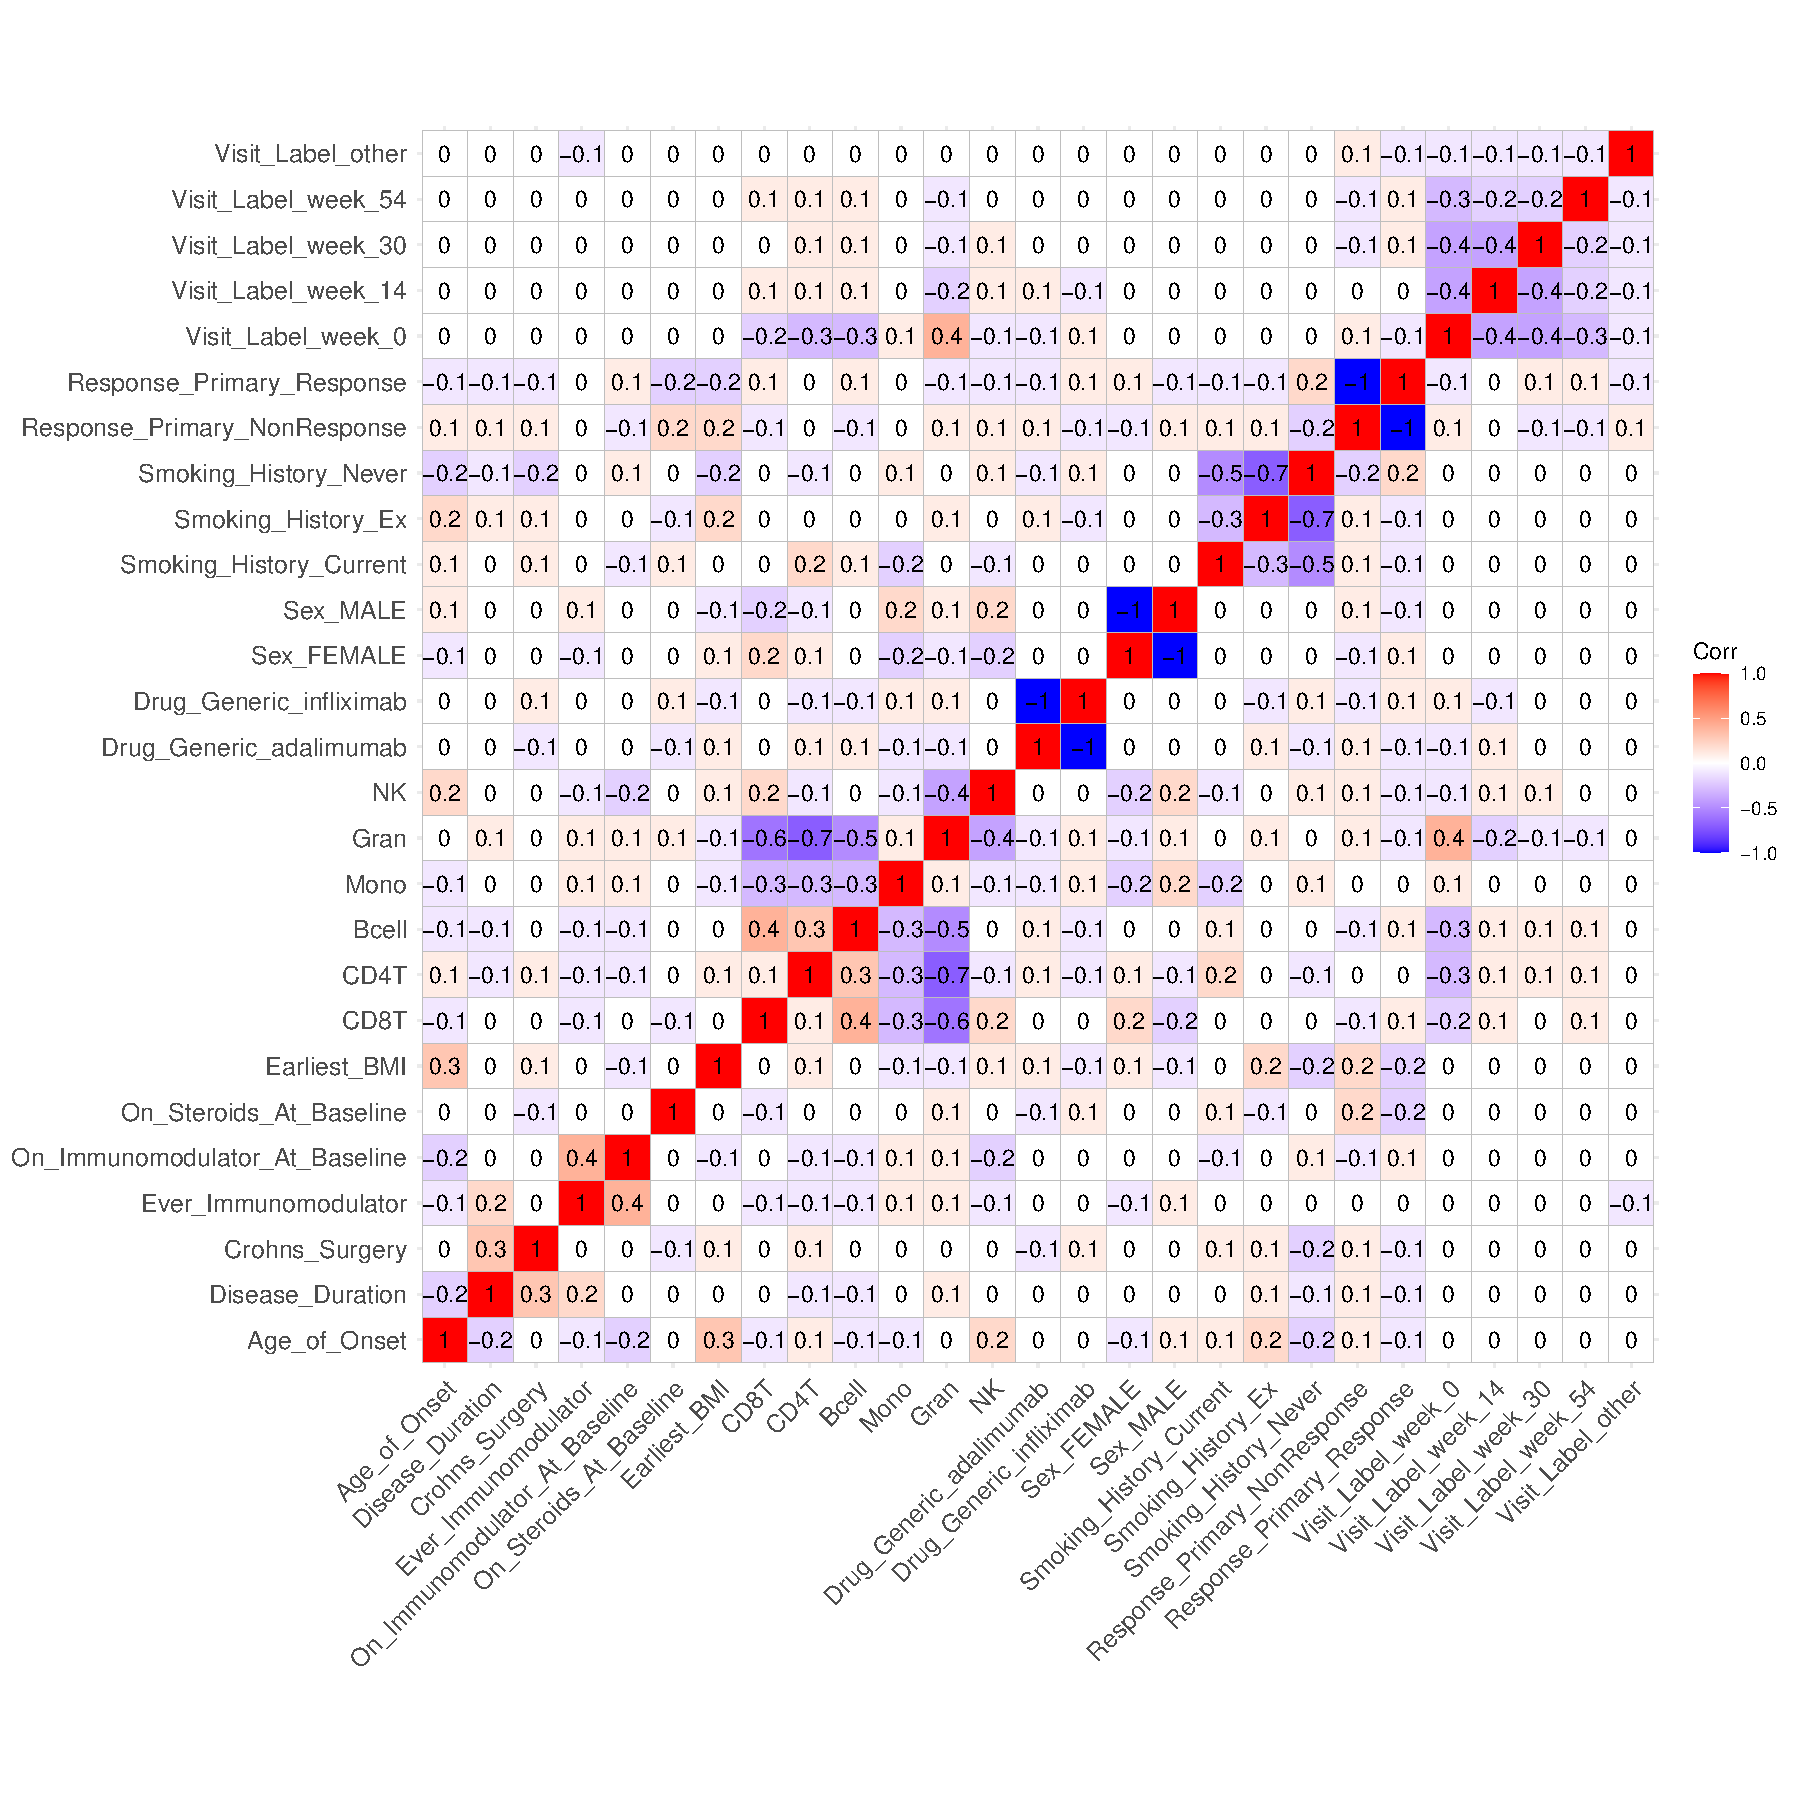
\includegraphics[width=1.0\textwidth,page=1]{mainmatter/figures/chapter_04/process_pheno.pheno_filtered_dge.ggcorrplot.pdf}
    \caption{Correlation matrix of phenotypes considered as independent variables in DGE and eQTL models.}
    \label{fig:multipants_pheno_filtered_ggcorrplot}
\end{figure}

% TODO: any need for plot?
\1 visualised main factors that influence global gene expression by PCA (\autoref{fig:multipants_dream_prcomp})
    \2 main separation along PC1 is w0 anti-TNF naive samples from all other post-drug start samples 
    \2 TODO: color other PCs by other variables: sex, response status, library prep protocol

% TODO: recolor to 1 page
\begin{figure}
    \centering
    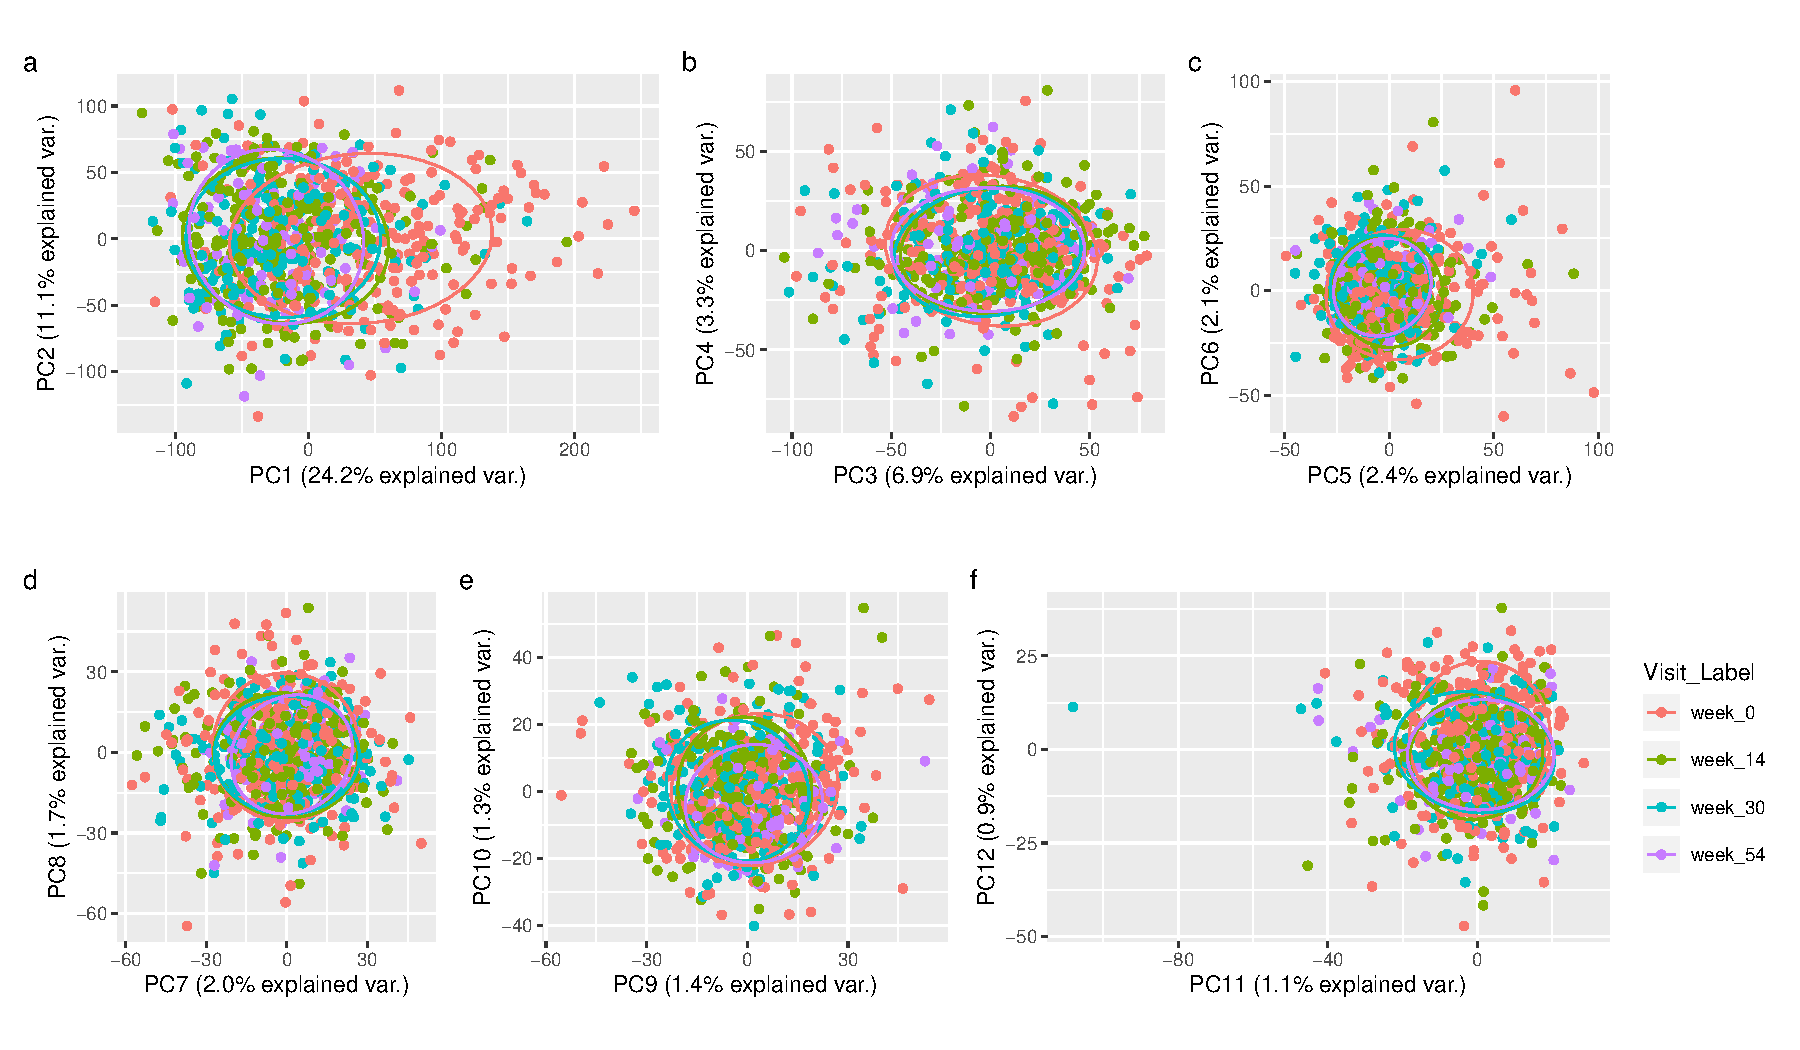
\includegraphics[width=1.0\textwidth,page=1]{mainmatter/figures/chapter_04/dream.prcomp.pdf}
    \caption{top 12 expression PCs of filtered expression data}
    \label{fig:multipants_dream_prcomp}
\end{figure}

\1 A variance components analysis was conducted to formally quantify the fractions of variation in expression explained by known variables
using \software{variancePartition}\autocite{hoffman2016VariancePartitionInterpretingDrivers}, which fits a mixed regression model.
% TODO covariates chosen here are used in all genewise models, we need a unified set.
Variables in \autoref{fig:multipants_pheno_filtered_ggcorrplot} were included as predictors.
    % Univariable analyses showed the strongest associations
    % with primary non-response to infliximab and
    % adalimumab were with week 14 drug and anti-drug
    % antibody concentrations (table 3; appendix p 17). Primary
    % non-response to infliximab was also associated with
    % older age at first dose, smoking at baseline, non-use of an
    % immunomodulator at baseline, lower baseline albumin
    % concentrations, and higher baseline white cell count.
    % Primary non-response to adalimumab was associated
    % with a higher body-mass index at baseline.
    \2 Includes prognostic factors from \autocite{kennedy2019PredictorsAntiTNFTreatment}
\1 Additional categorical variables were included for patient, \gls{RNAseq} plate, and library prep protocol version.
An additional continuous variable consisting of random numbers drawn from the standard normal distribution was also included as a null.
Granulocyte proportion estimates were dropped to relieve perfect multicollinearity.
Categorical variables were coded as random effects, and continuous variables as fixed effects.
Surprisingly, \textcite{hoffman2016VariancePartitionInterpretingDrivers} showed that variance proportion estimates are unbiased even when coding categorical variables with as few as two categories as random, 
as long as all model parameters are estimated jointly using \gls{ML} rather than \gls{REML}\footnote{
    \gls{REML} treats random effects as nuisance parameters and estimates fixed effects after first integrating out random effects).
}.
It was also shown that this approach also avoids over-estimates of variance proportions that occur if categorical variables with many levels are treated as fixed.

% aim to identify covariates, but will inevitably hit other types

\1 Variables were ranked by median variance proportion across all genes (\autoref{fig:multipants_varPart}).
The variables that explained the most variance included patient, cell proportions and \gls{RNAseq} plate.
    \2 most influential on interpretation are cell counts: there are pros and cons to using them
% should be given    special consideration as likely mediatgor
    \2 Cell proportions explain a lot of variance: this is expected \url{https://genome.cshlp.org/content/early/2020/06/24/gr.256735.119.abstract?papetoc} and even more so as they change a lot over time (\autoref{fig:multipants_cell_type_proportion_vs_Study_Day})
    \todo{anova for each cell prop over time for p values}
    \2 in the case of mediation i.e. PNR -> CC -> R
    \2 Should rarely find cell prop to be a collider, as in most genes, E -> cell prop is unlikely vs cell prop -> E
    \2 so keep them in as covariates
        \3 it's already popular for diff meth, and in DGE, can increase robustness \url{https://genomebiology.biomedcentral.com/articles/10.1186/s13059-019-1878-x}
    \2 note that we end up with the adjusted effect: upregulation in this context is increase in transcripts because making more per cell, not more in the bulk sample
        \3 this may not be ideal in prediction context, as each var input needs to be measured, and may even attenuate ability to predict \autocite{gaujoux2019CellcentredMetaanalysisReveals}
    \todo{don't know if it matters if there are colliders among covariates, since we can't estimate any causal effects in DGE due to lack of a control group?}

\begin{figure}
    \centering
    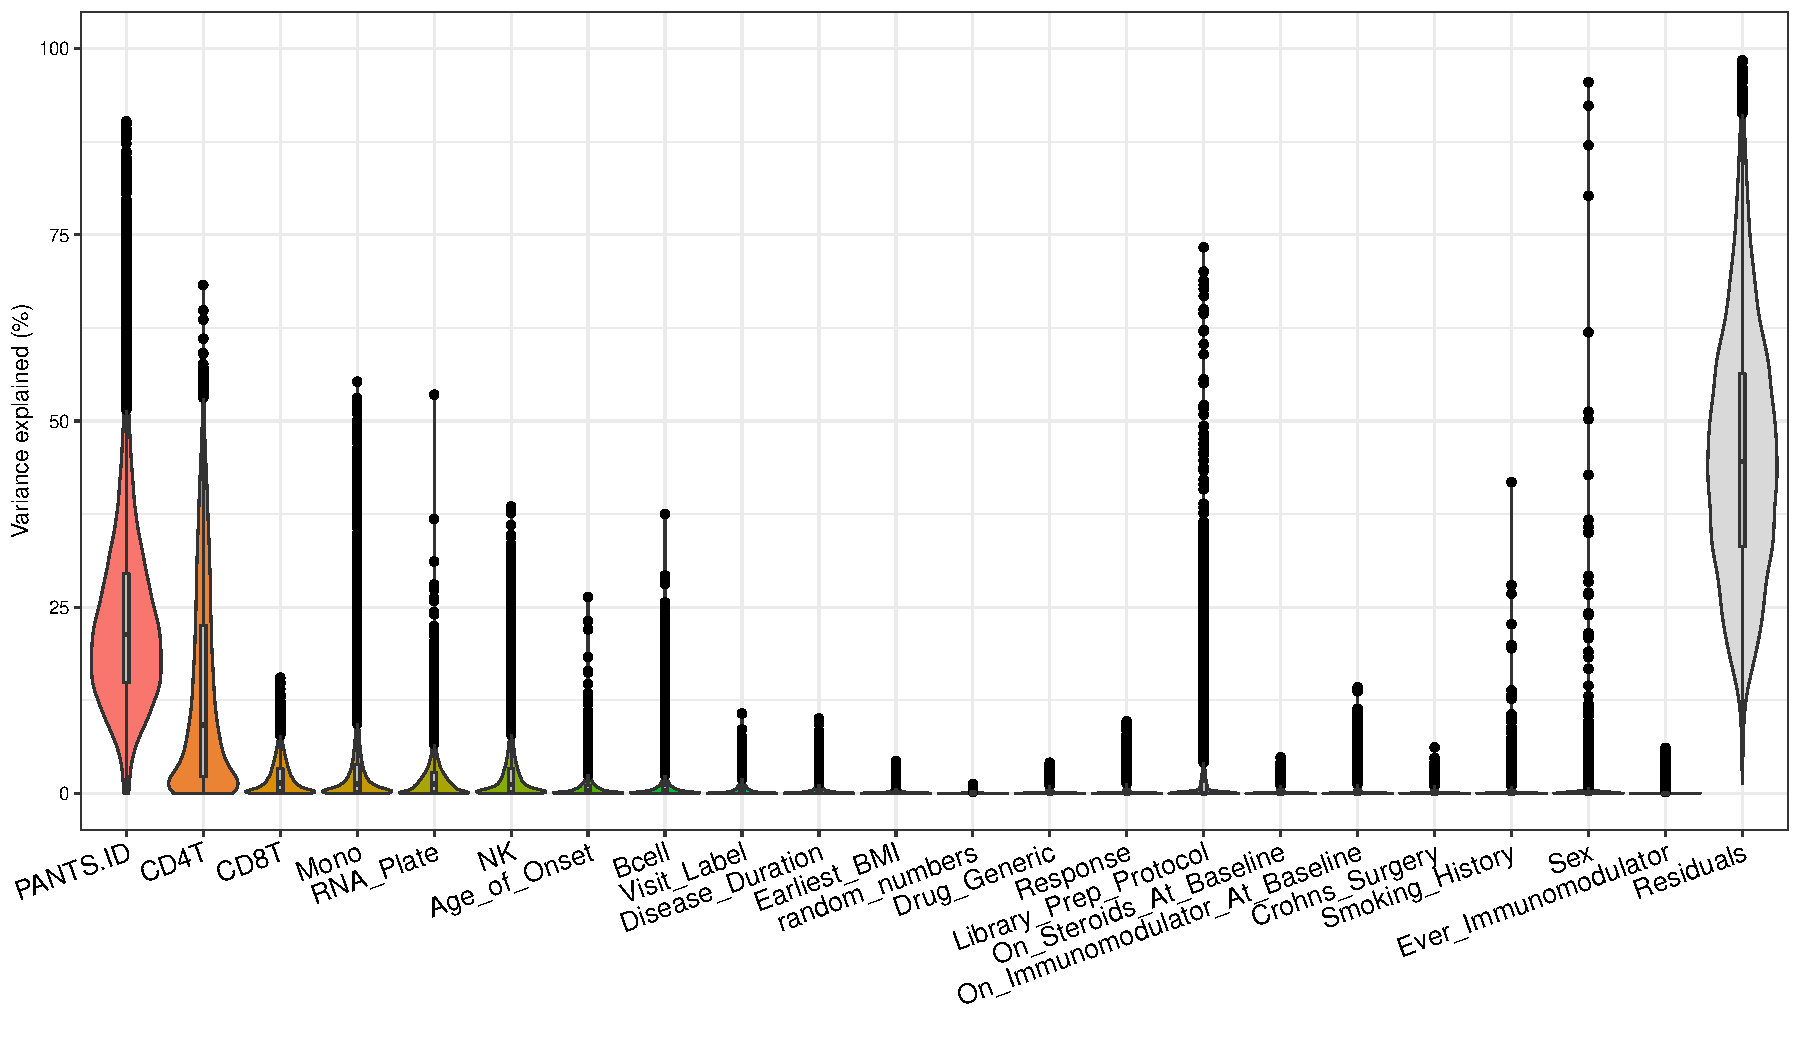
\includegraphics[width=1.0\textwidth,page=1]{mainmatter/figures/chapter_04/dream.plotVarPart.pdf}
    \caption{variance partition analysis, distribution of genewise \% variance in expression explained by each variable}
    \label{fig:multipants_varPart}
\end{figure}

\begin{figure}
    \centering
    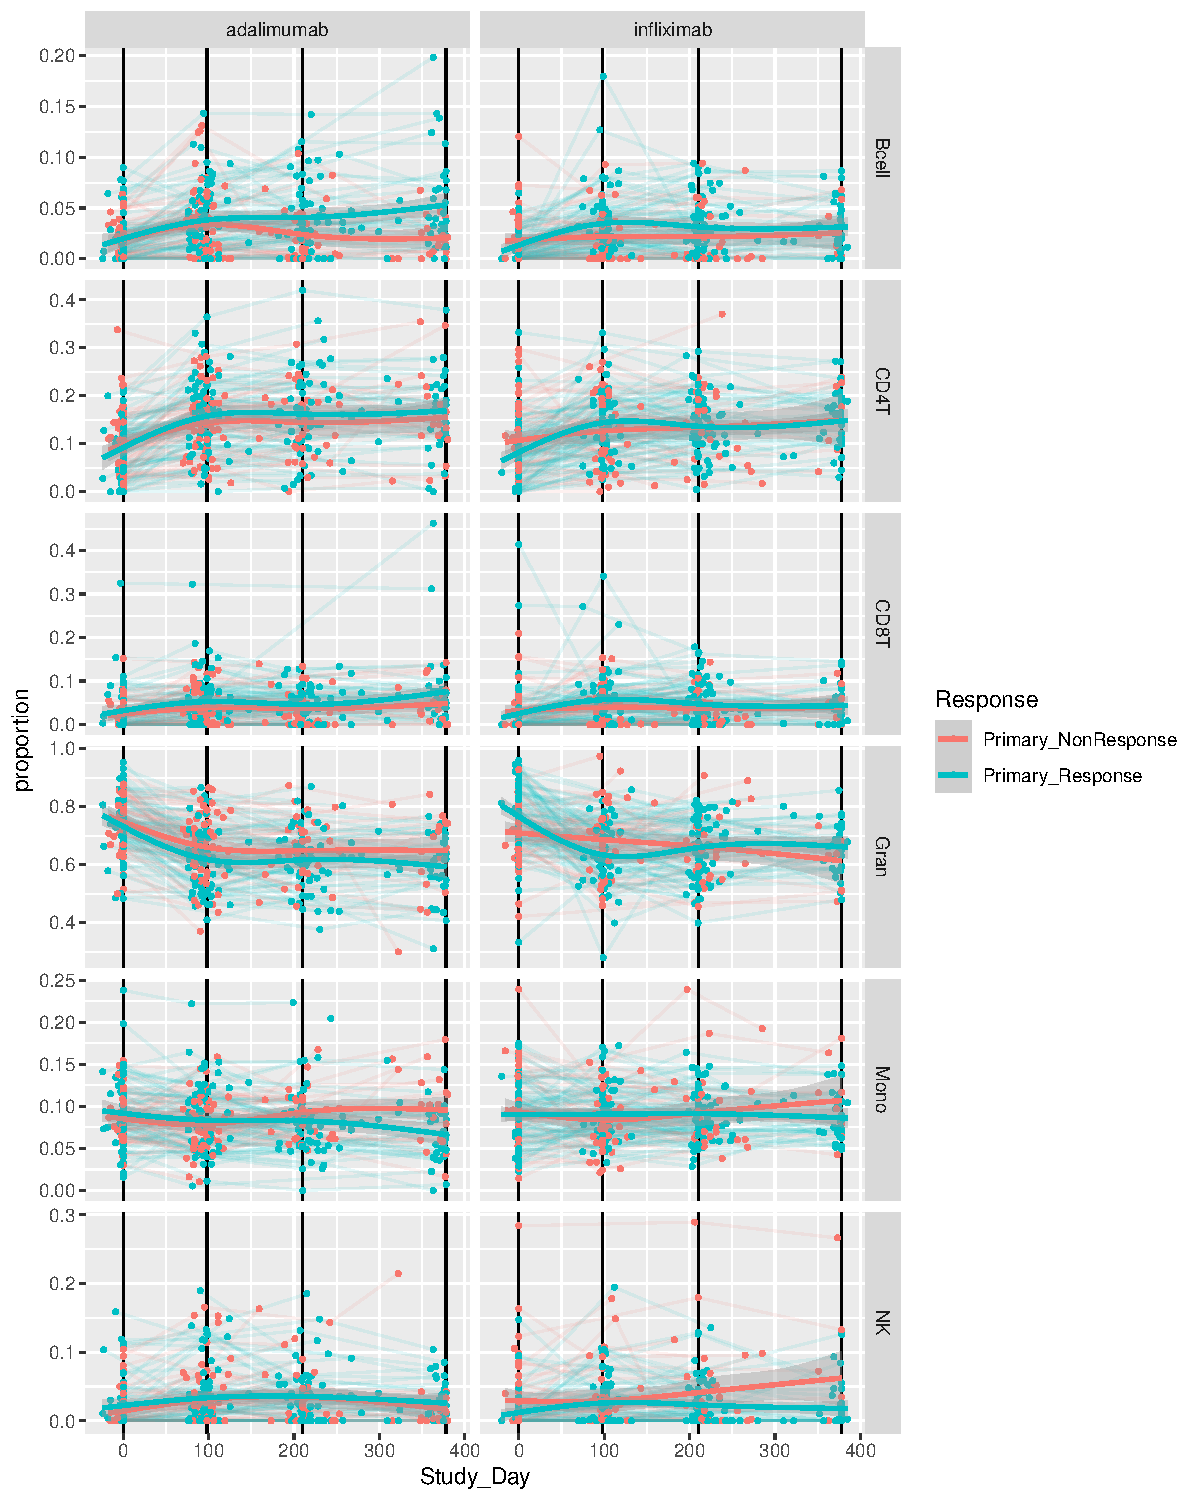
\includegraphics[width=1.0\textwidth,page=1]{mainmatter/figures/chapter_04/dream.cell_type_proportion_vs_Study_Day.pdf}
    \caption{changes in cell proportions of 6 immune cell types over time}
    \label{fig:multipants_cell_type_proportion_vs_Study_Day}
\end{figure}

\1 Variables that did not explain more variation on average than the null could still have high maximum values, 
    indicating their importance for specific genes only, such as genes with sex-specific expression.
    \2 would be best to customise per gene, but less comparable interpr between genes
    \2 Included, as we need a consensus set of covariates, and the penalty is only 1 df.
    \2 final list of covariates is [TODO: basically select all, except Gran, since we have proportions; and ever immunomodulator, which is low in median and max var explained]
    \todo{the var explained by Gran will be redistributed among highly cor vars anyways}
% Sex
% Age
% BMI
% Age of Onset
% Crohn’s Surgery
% Ever Immunomodulator
% Current Smoker
% Proportions of the 6 cell types: CD4+ T cells, CD8+ T cells, B cells, NK cells, monocytes, and granulocytes

\subsubsection{Contrasts for pairwise group comparisons}

\1 model form is E ~ [...] don't forget random fx!
\1 can we pool drugs with a mean term for this comparison? i.e. move from 8 to 4 means model
    \2 test interaction between drug and response at w0, and at w14 i.e. is there a diff in the diff between R vs NR between drugs?
    \2 no significant single gene hits at either timepoint
    \2 but unclear if preregistered power calculations would extend to this test \url{https://statmodeling.stat.columbia.edu/2018/03/15/need-16-times-sample-size-estimate-interaction-estimate-main-effect/}

    \2 there are baseline diffs are evident in clinical data \todo{because this is non-randomised, baseline differences do matter??}
    % Nick: “In general, sicker patients have often been given infliximab. At the time, children were rarely given adalimumab, but that doesn’t affect the RNA seq cohort because children were excluded.”
    \2 “Several baseline characteristics were significantly different between the infliximab-treated and adalimumab-treated patients, including age, smoking, body-mass index, disease duration, disease location, and disease behaviour. Patients treated with infliximab had more active disease at baseline than did patients treated with adalimumab, as evidenced by higher serum CRP and faecal calprotectin concentrations (table 1).” \autocite{kennedy2019PredictorsAntiTNFTreatment}
    \2 I include many but not all of these covariates in the DGE model

\1 used \software{dream} hoffman2018DreamPowerfulDifferential
\1 Group-means parametrisation with 8 means
    \2 equiv to to 3 way interactions between drug/response/visit
    \2 no intercept, so each group coef is a mean estimate
\1 specific hypotheses tested using sum to zero contrasts 
\1 Model also fit that used Group-means parametrisation with 4 means: pooling the two drugs
    % TODO
    % The grand mean or pooled mean is the mean of the means of several subsamples, as long as the subsamples have the same number of data points.
    % \2 note this is not the same as the same as the mean of means contrast as pooled is not mean of two means
\1 TODO: model equations
    \2 for dream analysis, unlike variancePartition, use REML over ML, so use fixed effects for small numbers of levels
    \2 also, need fixed effects for tested predictors
    % However, in the lme4 package in R the standards for evaluating significance of
    % fixed effects in these models (i.e., obtaining p-values) are somewhat vague.
    % There are good reasons for this, but as researchers who are using these models
    % are required in many cases to report p-values, some method for evaluating the
    % significance of the model output is needed.
    %
    % The primary motivation for this omission is that in linear mixed models it is
    % not at all obvious what the appropriate denominator degrees of freedom to use
    % are, except perhaps for some simple designs and nicely balanced data.
    \2 to get p values for papers, Dream uses lmerTest approximation Satterthwaite df \url{https://link.springer.com/article/10.3758/s13428-016-0809-y} with REML
    \2 this combo controls type 1 error for n>144 in lmerTest simulations
    \2 FDR BH separately per comparison: "The default method="separate" and adjust.method="BH" settings are appropriate for most analyses. method="global" is useful when it is important that the same t-statistic cutoff should correspond to statistical significance for all the contrasts." \url{https://rdrr.io/bioc/limma/man/decideTests.html}

\subsubsection{Spline model for difference over all timepoints}

% TODO there are methods, but did not use due to shortness of time series
% "Comparative analysis of differential gene expression tools for RNA sequencing time course data"
% Surprisingly, TC tools were outperformed by the classical pairwise comparison approach on short time series (<8 time points) in terms of overall performance and robustness to noise, mostly because of high number of false positives, with the exception of ImpulseDE2.

\1 aim is to uses info in samples from other timepoints, avoiding a large number of pairwise comparisons
    \2 a simple study day x responder interaction over time assumes linear change
\1 could aosl treat time as categorical visits (like baseline/w14 analysis above), then f test all interactions
    \2 but there is variation in study day in the visit windows

\1 spline model tests over all timepoints, are there diff trajectories for R and NR?
    \2 Internal Knots set at w14 and w30, since drug dose just after the visit, so slope should be allowed to change until next dose
    \2 cubic between knots, linear outside external knots
    \2 f test over 3 interaction terms between spline basis and study day
        \3 can include all data
        \3 TODO: read this for maths behind basis functions \url{https://bmcmedresmethodol.biomedcentral.com/articles/10.1186/s12874-019-0666-3}

        % FDR separate

% TODO
% f-test
% is a wald test
% https://support.bioconductor.org/p/6124/
% The above mentioned statistics are computed for every contrast for each gene. The eBayes() function computes one more useful statistic. The moderated F-statistic (F) combines the t-statistics for all the contrasts for each gene into an overall test of significance for that gene. The moderated F-statistic tests whether any of the contrasts are non-zero for that gene, i.e., whether that gene is differentially expressed on any contrast. The moderated-F has numerator degrees of freedom equal to the number of contrasts and denominator degrees of freedom the same as the moderated-t. Its p-value is stored as fit$F.p.value. It is similar to the ordinary F-statistic from analysis of variance except that the denominator mean squares are moderated across genes.

\1 TODO: clustering spline hits
    \2 note more accurate to use partial expression, but complicated for DREAM, so used unadjusted expression
    % center, no scale
    % pearson, which is scale invariant on centered data https://www.researchgate.net/publication/26290974_A_new_approach_for_clustering_gene_expression_time_series_data
    \2 Centroids defined by simple mean in each visit

\subsubsection{Gene set analysis ranked}

% camera is developed to use mod t, but in practice ranks are comparable between t and z.std, even though dream says otherwise
% https://bioconductor.org/packages/release/bioc/vignettes/variancePartition/inst/doc/dream.html#dream-analysis
\1 TODO: grab tmod paragraph from ch2
    \2 Genes are ranked by their test statistics, meaning we are ranking by significance
    % TODO
    % other more sophisticated ranking methods
    % Minimum Significant Difference \url{https://link.springer.com/article/10.1186/s12859-017-1674-0#Abs1} \url{https://cran.r-project.org/web/packages/tmod/vignettes/tmod.pdf}
    % treat method \url{http://web.mit.edu/~r/current/arch/i386_linux26/lib/R/library/limma/html/ebayes.html}
        \3 practice ranks are comparable between t and z.std, even though dream says otherwise, very high spearman cor
        % TODO: add spearman rank corr
    \2 approx 8k genes in the gene set annotation for tmod

The gene sets used were \glspl{BTM} from\autocite{li2013MolecularSignaturesAntibody}
"DC" (from Chaussabel et al. 2008)

\subsection{Genotyping and genotype data preprocessing}

% sazonovs2019HLADQA105Carriage
% DNA was extracted from pretreatment blood samples from
% 1524 patients in the PANTS cohort and genotyping undertaken
% using the Illumina CoreExome microarray
%
% After quality
% control, 1323 patients remained in the study, of which
% 1240 had drug and anti-drug antibody level data available
% (Supplementary Figure 2).
%
% 7,578,947 variants with an information content metric score .4 were subsequently taken forward for analysis
%
% HLA types were imputed at 2- and 4-digit resolution for the
% following loci: HLA-A, HLA-C, HLA-B, HLA-DRB1, HLA-DQA1,
% HLA-DQB1, and HLA-DPB1.
%
% sex,
% drug type (infliximab or adalimumab), immunomodulator use,
% and the first within-sample principal component were
% included as covariates (Supplementary Table 2).

\1 Whole blood samples were collected into EDTA tubes for genotypeing at w0
\1 TODO: scan Alex's thesis for genotyping and QC details
% TODO: check no batch effects e.g. chip, which would necc an insample PCA
    \2 autosomal only
    \2 TODO describe strange limix behaviour that lead to deduping visits by patient in sample filtering
    % although it may seem possible to have duplicate patients
    %     following the stacking logic of TODOcite,
    %     it estimation of the alternative model log likelihood
    %     excluding just a 2 duplicates at w14
    %     makes LL alt much lower
    %     LRT returns false negatives
    %
    %     resulting p value distribution is not well behaved:
    %     large spike at 1
    %
    %     but the betas and stes remain comparable
    %     since we use mashr to get signif values,
    %     can keep these in or out.


\subsection{Computing genotype PCs}

\1 used weights from akt for 1000G to do projection \autoref{fig:multipants_genotype_akt_1000g_pca}
    % just cases used. do not use in sample PCs?
    % TODO: read
        % Efficient toolkit implementing best practices for
        % principal component analysis of population
        % genetic data
    % would use FlashPCA2 if wanted to do myself e.g. between chip batches
\1 chose top 5 PCs for use in eQTL model
    \2 there is less pop structure here than HIRD. in HIRD, i did the PCA myself, and found 4 significant PCs with tracy-widom
    \2 from EIGENSTRAT paper, results not sensitive to number of PCs anyway, as long as it is sufficient \url{https://www.nature.com/articles/ng1847}
    % This implies that EIGENSTRAT results are not sensitive to the number of axes of variation used, as long as there is a sufficient number of axes to capture true population structure effects.
    % We see that in each SNP category, results are virtually identical for K = 1, 2, 5 or 10.

\begin{figure}
    \centering
    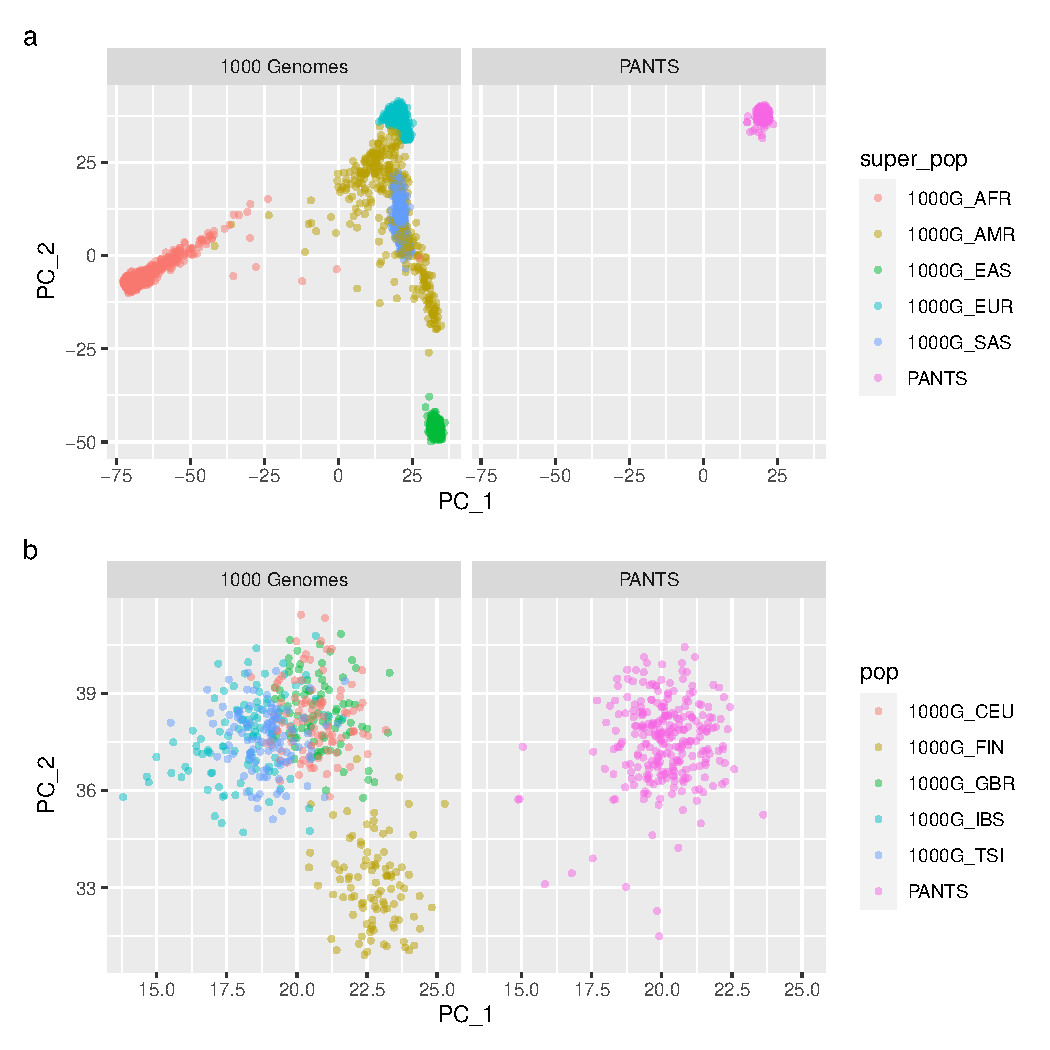
\includegraphics[width=1.0\textwidth,page=1]{mainmatter/figures/chapter_04/pants_samples.sampleids_cleaned_to_lowercase.filtered.GRCh38.sorted.multiPANTS.projection_1000G_pca.pdf}
    \caption{projection of PANTS samples onto 1000G genotype PC axes}
    \label{fig:multipants_genotype_akt_1000g_pca}
\end{figure}

\subsection{reQTL analysis}

\1 same overall strat as ch3

% Alternative:
% In the ANCOVA approach, the whole focus is on whether one group has a higher mean after the treatment. It’s appropriate when the research question is not about gains, growth, or changes.

% https://www.theanalysisfactor.com/pre-post-data-repeated-measures/
% ANCOVA vs repeated measures vs mixed model

% The biggest advantage of mixed models is their incredible flexibility.  They can handle clustered patients as well as repeated measures (even in the same model).  They can handle crossed random effects, where there are repeated measures not only on an patient, but also on each stimulus.
% https://www.theanalysisfactor.com/repeated-measures-approaches/

% Then work out if genetics changes trajectories for any gene i.e. DGE models with a snp as predictor
% First need to eQTL scan in general with mashr and find the snps in the most reQTLish genes, since this modelling is probably expensive

\subsubsection{Finding hidden confounders in expression data}

\1 PEER (same as ch3)
    \2 Used DESeq2 vst for between sample norm e.g. sequencing depth 
    \2 Chose n PEER to maximise cis-eQTLs on chr1 \autoref{fig:multipants_reqtl_PEER_k_choice} 

\begin{figure}
    \centering
    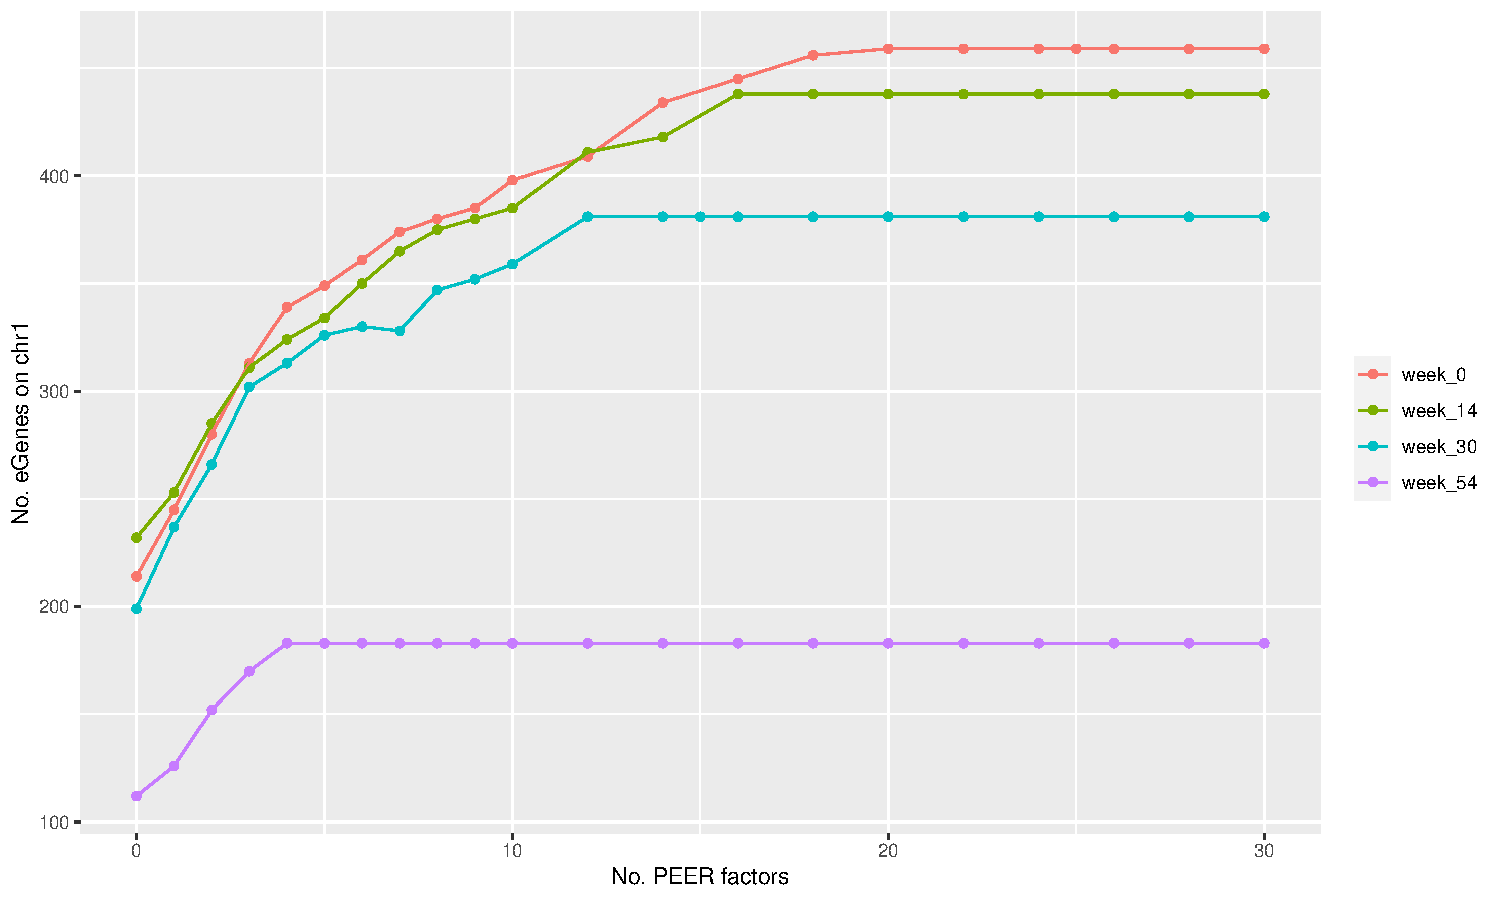
\includegraphics[width=1.0\textwidth,page=1]{mainmatter/figures/chapter_04/count_eGenes.signif_eGenes_vs_PEER_n.dataset_multiPANTS.chr_1.pdf}
    \caption{number of eGenes on chr1 used to choose number of PEER factors for each timepoint}
    \label{fig:multipants_reqtl_PEER_k_choice}
\end{figure}

\subsubsection{Computing GRMs}

\1 LDAK, same as ch3

\subsubsection{limix model}

\1 same as ch3, limix
    \2 n at each timepoint was [...]
    \2 AC thresh 15
    \2 extra filter to avoid small numbers of minor hom, as without sufficient numbers, leads to data points with high leverage that may be unduely influential on the beta
    % despite mashr migitation by shrinkage? is it sufficient?
    % when the whole point is calling signif changes in beta
    \2 used a >5 min hom filter
        % gated by lowest n among 4 visits, but 15 to 25 MAF diff only

\1 find lead eQTL for each gene in any condition by lowest lfsr
    \2 breaking ties by highest imputation INFO, highest \gls{MAF}, shortest dist to \gls{TSS}, and genomic coordinate.

\subsubsection{mashr joint analysis}

\1 same as ch3
    \2 TODO describe mashr bug for negative betas
    \2 reQTLs defined by difference in betas test between timepoints
    \2 BH FDR separate per comparison, not globally

\subsubsection{Clustering reQTLs}

% TODO
% Clustering time-course Microarray data using functional Bayesian innite mixture model
% clustering folder in downloads
% https://2-bitbio.com/2017/04/clustering-rnaseq-data-making-heatmaps.html
% https://hbctraining.github.io/DGE_workshop/lessons/08_DGE_LRT.html

\1 <pipeline>
    \2 align
    \2 Centering, no scaling
        \3 ensure comparability between gene
        \3 Amplifies noise? Migitate by prefiltering on nominal signif diff between two timepoints
    % https://hdbscan.readthedocs.io/en/latest/comparing_clustering_algorithms.html
    \2 dist\_cor(method='pearson')
    \2 fastcluster::hclust(method='complete')
    \2 distance metric 1-cor(pearson)
    % •	https://www.rdocumentation.org/packages/NbClust/versions/3.0/topics/NbClust
    % o	Possible statistics: the index to be calculated. This should be one of : "kl", "ch", "hartigan", "ccc", "scott", "marriot", "trcovw", "tracew", "friedman", "rubin", "cindex", "db", "silhouette", "duda", "pseudot2", "beale", "ratkowsky", "ball", "ptbiserial", "gap", "frey", "mcclain", "gamma", "gplus", "tau", "dunn", "hubert", "sdindex", "dindex", "sdbw", "all" (all indices except GAP, Gamma, Gplus and Tau), "alllong" (all indices with Gap, Gamma, Gplus and Tau included).
    \2 Number of clusters: gap stat fviz\_nbclust

\subsubsection{gprofiler}

\section{Results}
\todo{what to put in results vs discussion. going with the pattern of providing enough info for the reader to intepret the data in the results, then doing a summary and my own interpretation in the discussion}

\subsection{Longitudinal \glsfmtshort{RNAseq} data from the \gls{PANTS} cohort}

To define transcriptomic differences between primary responders and non-responders to anti-gls{TNF} therapy in the \gls{PANTS} cohort, 
I analysed whole blood \gls{RNAseq} gene expression measured at up to four timepoints per patient:
week 0 baseline before commencing anti-gls{TNF} therapy, and weeks 14, 30 and 54 after commencing anti-gls{TNF} therapy.
After quality control, expression data was available for 15584 genes and 814 samples (\autoref{fig:multipants_studyDay_boxplots}).
These samples come from 324 patients, with a median of three samples per patient (\autoref{fig:multipants_visits_upset}).

Patient characteristics are shown in \autoref{tab:multipants_table1}. \todo{autoref to table 1}
The proportion of primary non-responders is high (43.8\%) compared to the overall proportion in the \gls{PANTS} cohort (23.8\%)\autocite{kennedy2019PredictorsAntiTNFTreatment}.
This is due to sample selection for \gls{RNAseq} to balance the sample size for each combination of drug and primary response status.

\begin{figure}
    \centering
    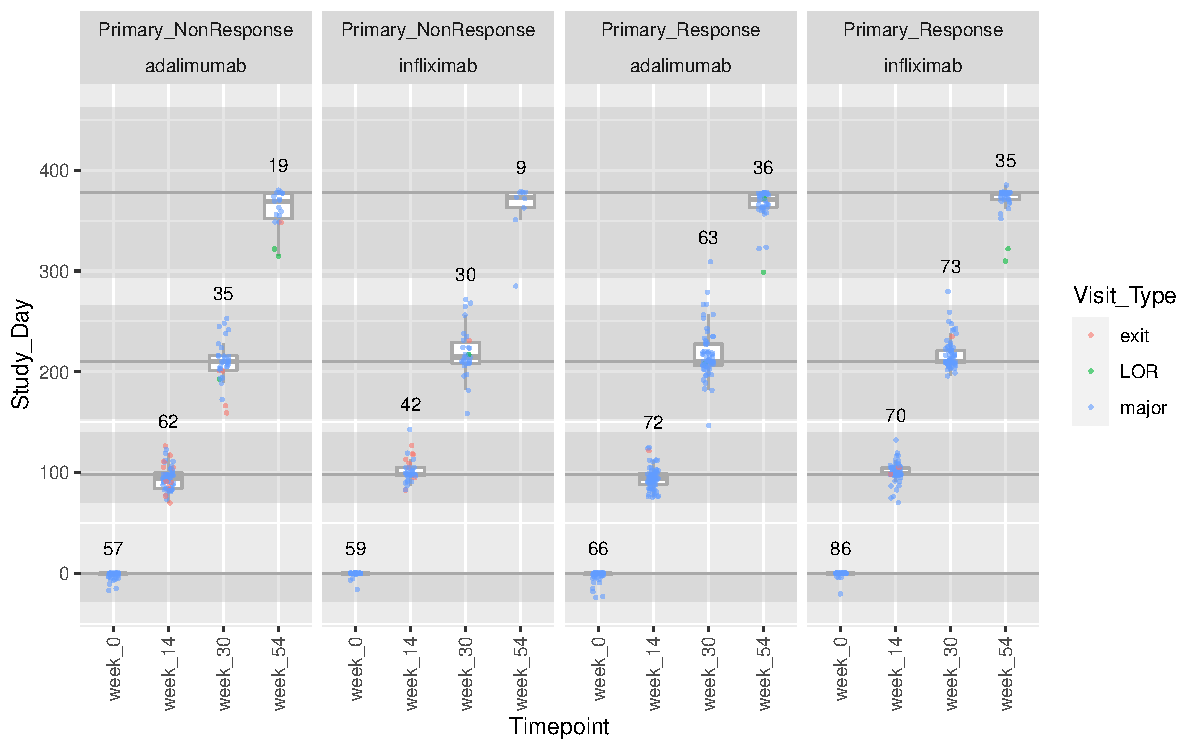
\includegraphics[width=1.0\textwidth,page=1]{mainmatter/figures/chapter_04/process_pheno.pheno_filtered_dge.Study_Day_vs_Visit_Label.pdf}
    \caption{Distribution of samples among defined study visit windows. lor and exit are additional visits that fall into the windows.}
    \label{fig:multipants_studyDay_boxplots}
\end{figure}

\begin{figure}
    \centering
    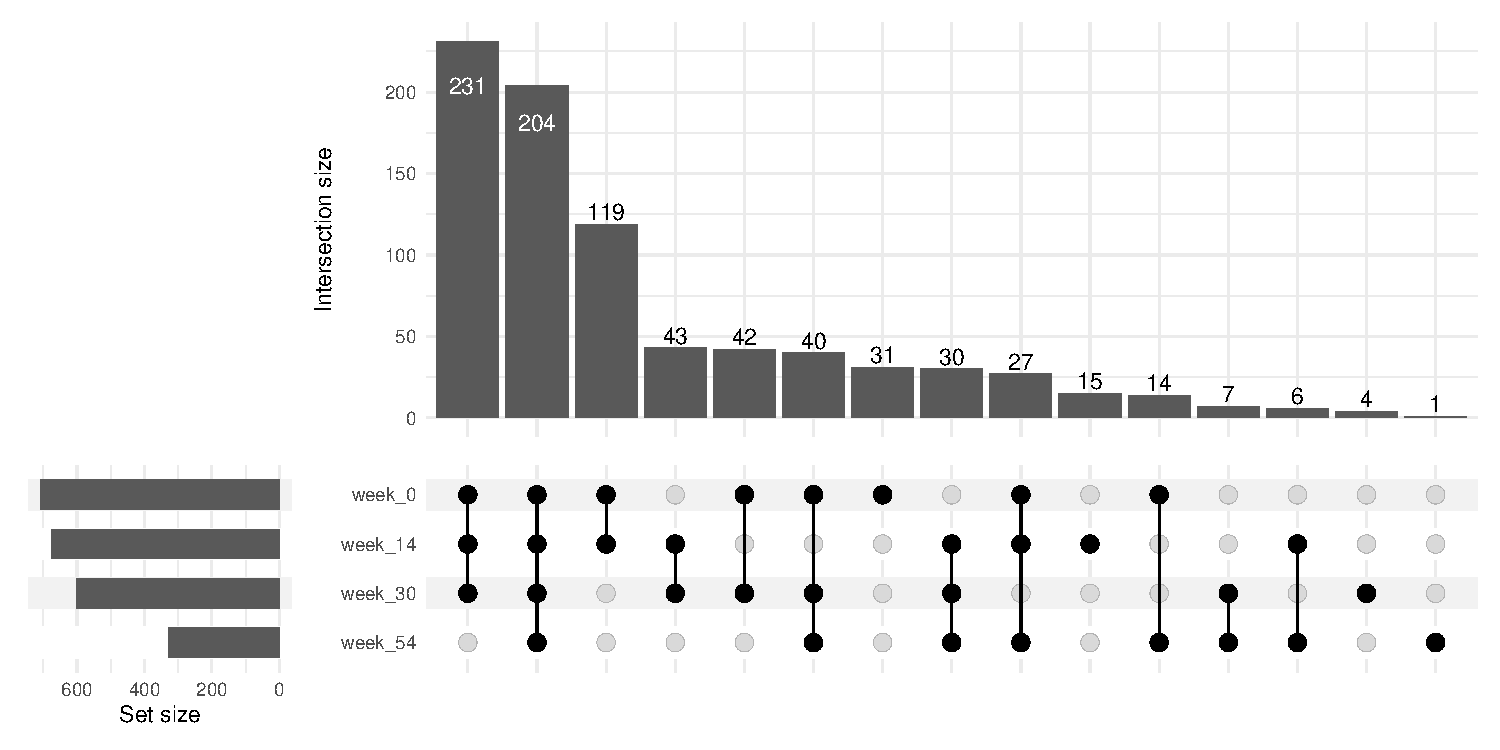
\includegraphics[width=1.0\textwidth,page=1]{mainmatter/figures/chapter_04/process_pheno.pheno_filtered_dge.Visit_Label_upset.pdf}
    \caption{}
    \label{fig:multipants_visits_upset}
\end{figure}

% TODO: add caption and label
% \caption{Patient demographic and clinical characteristics.}\label{tab:multipants_table1}
% \begin{adjustbox}{width=\textwidth}
% \end{adjustbox}
% Table 1. 
% latex table generated in R 3.6.2 by xtable 1.8-4 package
% Fri Sep  4 19:08:12 2020
\begin{table}[]
\centering
\caption[\captionshort{Patient characteristics for the \gls{PANTS} \gls{RNAseq} subcohort.}]{\textbf{Patient characteristics for the \gls{PANTS} \gls{RNAseq} subcohort.} Values are count and percentage for categorical variables; mean and standard deviation for continuous variables; \pvalues{} are for the comparison between drugs.}\label{tab:multipants_table1}
\begin{adjustbox}{width=0.9\textwidth,height=0.9\textheight,keepaspectratio}
\begin{tabular}{lrrrr}
  \hline
  & adalimumab (ADA) & infliximab (IFX) & drugs pooled & p-value \\ 
  \hline
\textbf{Sex      } &  &  &  & 0.317 \\ 
  \hskip .5cm   (Col \%) &  &  &  & Fisher exact \\ 
  \hskip .5cm   FEMALE & 78 (48.4\%) & 89 (54.6\%) & 167 (51.5\%) &  \\ 
  \hskip .5cm   MALE & 83 (51.6\%) & 74 (45.4\%) & 157 (48.5\%) &  \\ 
    \textbf{Age of onset (years)      } &  &  &  & 0.774 \\ 
  \hskip .5cm    Mean (SD) & 33.3 (15.4) & 32.8 (15.3) & 33.1 (15.3) & Wilcoxon rank-sum \\ 
  \hskip .5cm    Missing & 0 & 0 & 0 &  \\ 
    \textbf{Disease duration (years)      } &  &  &  & 0.546 \\ 
  \hskip .5cm    Mean (SD) & 6.1 (8.1) & 5.9 (7.7) & 6.0 (7.9) & Wilcoxon rank-sum \\ 
  \hskip .5cm    Missing & 0 & 0 & 0 &  \\ 
    \textbf{Smoking status      } &  &  &  & 0.263 \\ 
  \hskip .5cm   (Col \%) &  &  &  & Fisher exact \\ 
  \hskip .5cm   Current & 28 (17.4\%) & 36 (22.1\%) & 64 (19.8\%) &  \\ 
  \hskip .5cm   Ex & 55 (34.2\%) & 43 (26.4\%) & 98 (30.2\%) &  \\ 
  \hskip .5cm   Never & 78 (48.4\%) & 84 (51.5\%) & 162 (50.0\%) &  \\ 
    \textbf{Crohn's-related surgery      } &  &  &  & 0.549 \\ 
  \hskip .5cm   (Col \%) &  &  &  & Fisher exact \\ 
  \hskip .5cm   FALSE & 114 (70.8\%) & 110 (67.5\%) & 224 (69.1\%) &  \\ 
  \hskip .5cm   TRUE & 47 (29.2\%) & 53 (32.5\%) & 100 (30.9\%) &  \\ 
    \textbf{On immunomodulator ever      } &  &  &  & 0.543 \\ 
  \hskip .5cm   (Col \%) &  &  &  & Fisher exact \\ 
  \hskip .5cm   FALSE & 23 (14.3\%) & 28 (17.2\%) & 51 (15.7\%) &  \\ 
  \hskip .5cm   TRUE & 138 (85.7\%) & 135 (82.8\%) & 273 (84.3\%) &  \\ 
    \textbf{On immunomodulator at baseline      } &  &  &  & 0.912 \\ 
  \hskip .5cm   (Col \%) &  &  &  & Fisher exact \\ 
  \hskip .5cm   FALSE & 79 (49.1\%) & 81 (49.7\%) & 160 (49.4\%) &  \\ 
  \hskip .5cm   TRUE & 82 (50.9\%) & 82 (50.3\%) & 164 (50.6\%) &  \\ 
    \textbf{On corticosteroids at baseline      } &  &  &  & 0.011 \\ 
  \hskip .5cm   (Col \%) &  &  &  & Fisher exact \\ 
  \hskip .5cm   FALSE & 113 (70.2\%) & 92 (56.4\%) & 205 (63.3\%) &  \\ 
  \hskip .5cm   TRUE & 48 (29.8\%) & 71 (43.6\%) & 119 (36.7\%) &  \\ 
    \textbf{Baseline BMI      } &  &  &  & 0.237 \\ 
  \hskip .5cm    Mean (SD) & 25.2 (6.2) & 24.3 (5.5) & 24.8 (5.9) & Wilcoxon rank-sum \\ 
  \hskip .5cm    Missing & 0 & 0 & 0 &  \\ 
    \textbf{Primary response status      } &  &  &  & 0.263 \\ 
  \hskip .5cm   (Col \%) &  &  &  & Fisher exact \\ 
  \hskip .5cm   Primary non-response & 76 (47.2\%) & 66 (40.5\%) & 142 (43.8\%) &  \\ 
  \hskip .5cm   Primary response & 85 (52.8\%) & 97 (59.5\%) & 182 (56.2\%) &  \\ 
    \textbf{CD8+ T cell (\%)      } &  &  &  & 0.380 \\ 
  \hskip .5cm    Mean (SD) & 2.8 (4.2) & 2.8 (5.2) & 2.8 (4.7) & Wilcoxon rank-sum \\ 
  \hskip .5cm    Missing & 38 & 18 & 56 &  \\ 
    \textbf{CD4+ T cell (\%s)      } &  &  &  & 0.752 \\ 
  \hskip .5cm    Mean (SD) & 9.2 (6.3) & 9.2 (6.8) & 9.2 (6.5) & Wilcoxon rank-sum \\ 
  \hskip .5cm    Missing & 38 & 18 & 56 &  \\ 
    \textbf{B cell (\%s)      } &  &  &  & 0.094 \\ 
  \hskip .5cm    Mean (SD) & 1.9 (2.0) & 1.5 (1.9) & 1.7 (1.9) & Wilcoxon rank-sum \\ 
  \hskip .5cm    Missing & 38 & 18 & 56 &  \\ 
    \textbf{Monocyte (\%s)      } &  &  &  & 0.497 \\ 
  \hskip .5cm    Mean (SD) & 8.9 (3.5) & 9.2 (3.7) & 9.0 (3.6) & Wilcoxon rank-sum \\ 
  \hskip .5cm    Missing & 38 & 18 & 56 &  \\ 
    \textbf{NK cell (\%s)      } &  &  &  & 0.683 \\ 
  \hskip .5cm    Mean (SD) & 1.9 (3.2) & 1.9 (3.8) & 1.9 (3.5) & Wilcoxon rank-sum \\ 
  \hskip .5cm    Missing & 38 & 18 & 56 &  \\ 
    \textbf{Granulocyte (\%s)      } &  &  &  & 0.911 \\ 
  \hskip .5cm    Mean (SD) & 74.3 ( 9.7) & 74.3 (10.8) & 74.3 (10.3) & Wilcoxon rank-sum \\ 
  \hskip .5cm    Missing & 38 & 18 & 56 &  \\ 
     \hline
\end{tabular}
\end{adjustbox}
\end{table}



\subsection{Gene expression associated with primary response at baseline}

Patient primary response to anti-\gls{TNF} was defined after the induction period, between week 12 and week 14 according to the clinical decision algorithm from \autocite{kennedy2019PredictorsAntiTNFTreatment} described in \autoref{multiPANTS:PR_definition}, 
which integrates clinician assessment with change in \gls{CRP} level and \gls{HBI} score.
To identify differences in baseline gene expression associated with future primary response, 
I fit gene-wise linear models at 15511 genes, comparing week 0 gene expression in primary responders with primary non-responders.
Comparisons were performed both within infliximab-only and adalimumab-only subgroups, and with both drugs pooled.
Models were run both adjusting for cell composition estimates of six immune cell types, and without adjustment.
Throughout this section, the significance threshold was set at FDR < 0.05 for each comparison, and upregulation refers to increased expression in primary responders versus non-responders.

Without adjusting for cell composition, the largest effects were infliximab-only, with 859 genes differentially expressed.
Only \gene{KCNN3} (log2FC=\num{-0.843455423}) was significant for the adalimumab-only comparison, 
% logFC      AveExpr         t      P.Value   adj.P.Val     z.std
% 0.34597454 6.55605 4.9264804 1.094745e-06 0.016980595 4.8737951
% 0.31379161 6.55605 4.6913403 3.384743e-06 0.050291627 4.6459748
and only \gene{SIGLEC10} (log2FC=\num{0.34597454}) was significant in the pooled analysis (\autoref{fig:multipants_dge_volcano_week_0_R_N}).

After adjustment for cell composition, there were no longer any significant infliximab-only genes, 
with 856/859 genes that were significant before the comparison having a dampened effect size after correction (smaller absolute effect and same sign), suggesting many effects may be mediated by cell composition.
\gene{SIGLEC10} in the combined analysis was also non-significant after adjustment (adjusted log2FC=\num{0.31379161}, FDR=\num{0.050291627}).
Conversely, at three genes downregulated in the adalimumab-only analysis that were the only significant genes post-adjustment, I observed increased significance:
%       logFC  AveExpr          t      P.Value  adj.P.Val      z.std
% -0.33495771 2.569096 -4.5040835 7.723531e-06 0.05989985 -4.4727077
% -0.35115926 2.569096 -5.0627658 5.212334e-07 0.00677703 -5.0183272
\gene{PDIA5} (unadjusted log2FC=\num{-0.33495771}, adjusted log2FC=\num{-0.35115926}), 
% -0.843455423 -0.2360221 -4.7304059 2.689467e-06 0.04171633 -4.69321336
% -0.879776701 -0.2360221 -4.9610155 8.738353e-07 0.00677703 -4.91811062
\gene{KCNN3} (\num{-0.843455423}, \num{-0.879776701}), 
% -1.1529588 1.169468 -4.212961 2.854891e-05 0.1476074 -4.184743
% -1.2231591 1.169468 -4.479679 8.738258e-06 0.0451797 -4.446249
and \gene{IGKV1-9} (\num{-1.1529588}, \num{-1.2231591}).
\todo{The role of cell composition estimates here may be more akin to precision variables. could be suppression, but hard to tell with n=3 hits to work with, in any case, formal tests for difference in effect between adjusted and non-adjusted estimates were not performed}

To identify coordinately up and downregulated gene sets and increase sensitivity for detecting differences between primary responders and non-responders,
I performed ranked gene set analysis on the gene-wise z-statistics using blood transcriptomic modules: annotated sets of coexpressed genes in peripheral whole blood.
This module-level analysis was also run unadjusted (\autoref{fig:multipants_dge_panelPlot_week_0_R_N_cellPropF}) and adjusted for cell composition (\autoref{fig:multipants_dge_panelPlot_week_0_R_N_cellPropT}).

Despite only \gene{SAMD10} having a significantly different effect between drugs at the gene-level (an interaction between drug and response at week 0), 
the large global differences observable in \autoref{fig:multipants_dge_volcano_week_0_R_N} were detected in the module-level analysis\footnote{It is likely the study is not powered to detect gene-level three-way interaction effects between timepoint, drug and response, although I am not aware of which subgroup analyses may have been prespecified during the study design and sample size calculations for the \gls{PANTS} \gls{RNAseq} cohort.}.
Without adjusting for cell composition, many of the most significantly upregulated modules in the pooled analysis, 
including upregulation of monocyte (LI.M11.0, LI.S4) and neutrophil modules (LI.M37.1, LI.M11.2),
appear to be driven by infliximab.
These modules have heavily reduced significance after adjusting for cell composition.
The new modules that are most upregulated in the pooled analysis after adjustment:
MHC-TLR7-TLR8 cluster (LI.M146), antigen presentation (LI.M71, LI.M95.0), and myeloid cell enriched receptors and transporters (LI.M4.3),
have more consistent effects between drugs.

For downregulated modules before adjustment, I observed
adalimumab-specific effects for
plasma cells, B cells and immunoglobulin modules (LI.M156.0, LI.M156.0, LI.S3); and cell cycle and transcription modules (LI.M4.0, LI.M4.1).
Infliximab-specific effects were observed for NK cell (LI.M7.2) and T cell (LI.M7.0, LI.M7.1) modules.
The significance of these modules is also reduced after adjusting for cell composition,
but they remain the most significantly downregulated modules.

\begin{figure}
    \centering
    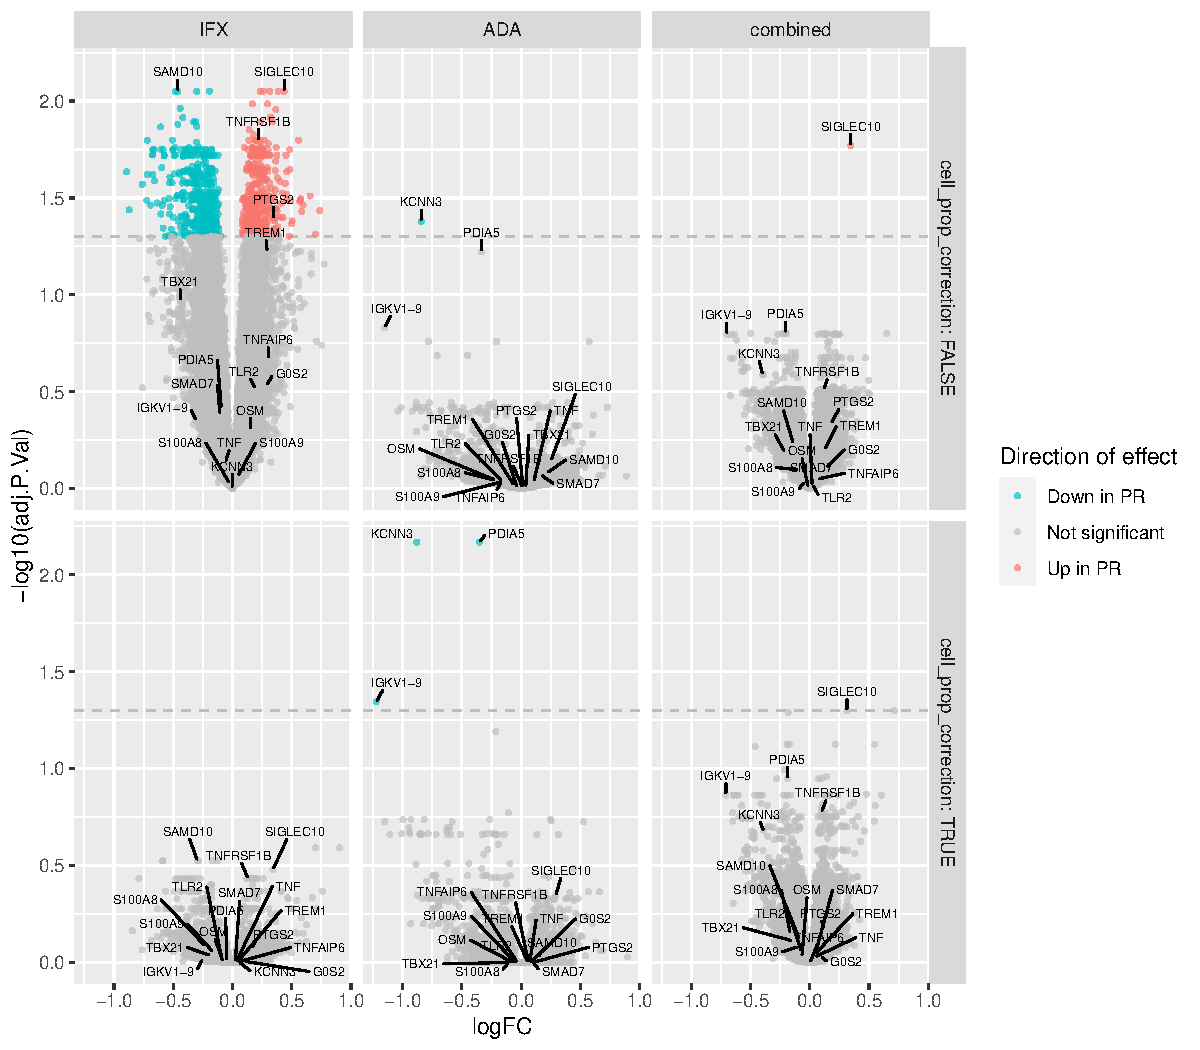
\includegraphics[width=1.0\textwidth,page=1]{mainmatter/figures/chapter_04/plot_gene_set_enrichment.dge_result_volcano_simple_C_1RI_1NI,C_1RA_1NA,C_1R_1N.pdf}
    \caption{DGE volcano plot for PR vs PNR at week 0}
    \label{fig:multipants_dge_volcano_week_0_R_N}
\end{figure}

% \begin{figure}
%     \centering
%     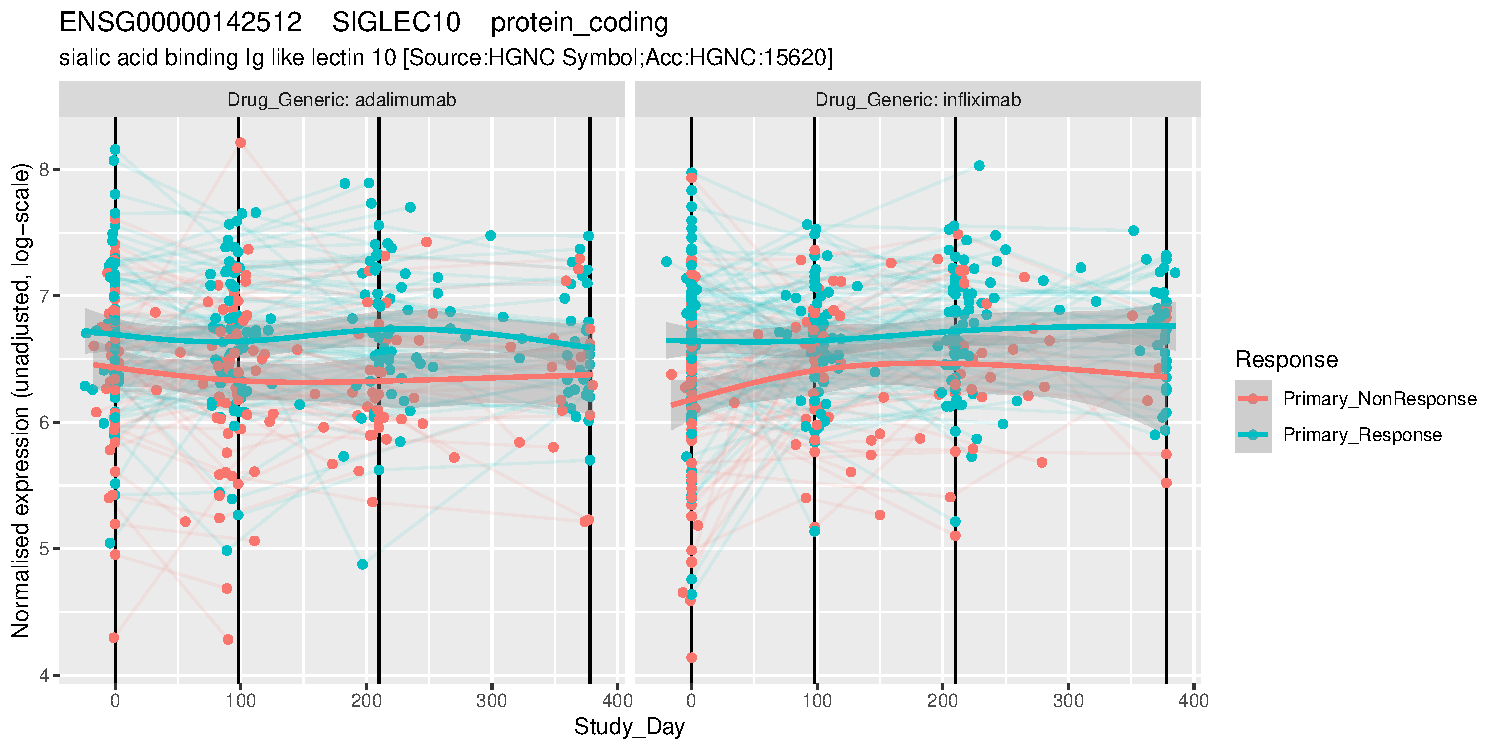
\includegraphics[width=1.0\textwidth,page=1]{mainmatter/figures/chapter_04/dream.E_vs_Study_Day.GENEID_ENSG00000142512.SYMBOL_SIGLEC10.pdf}
%     \caption{Unadjusted, normalised SIGLEC10 expression over time}
%     \label{fig:multipants_dge_SIGLEC10}
% \end{figure}

\begin{figure}
    \centering
    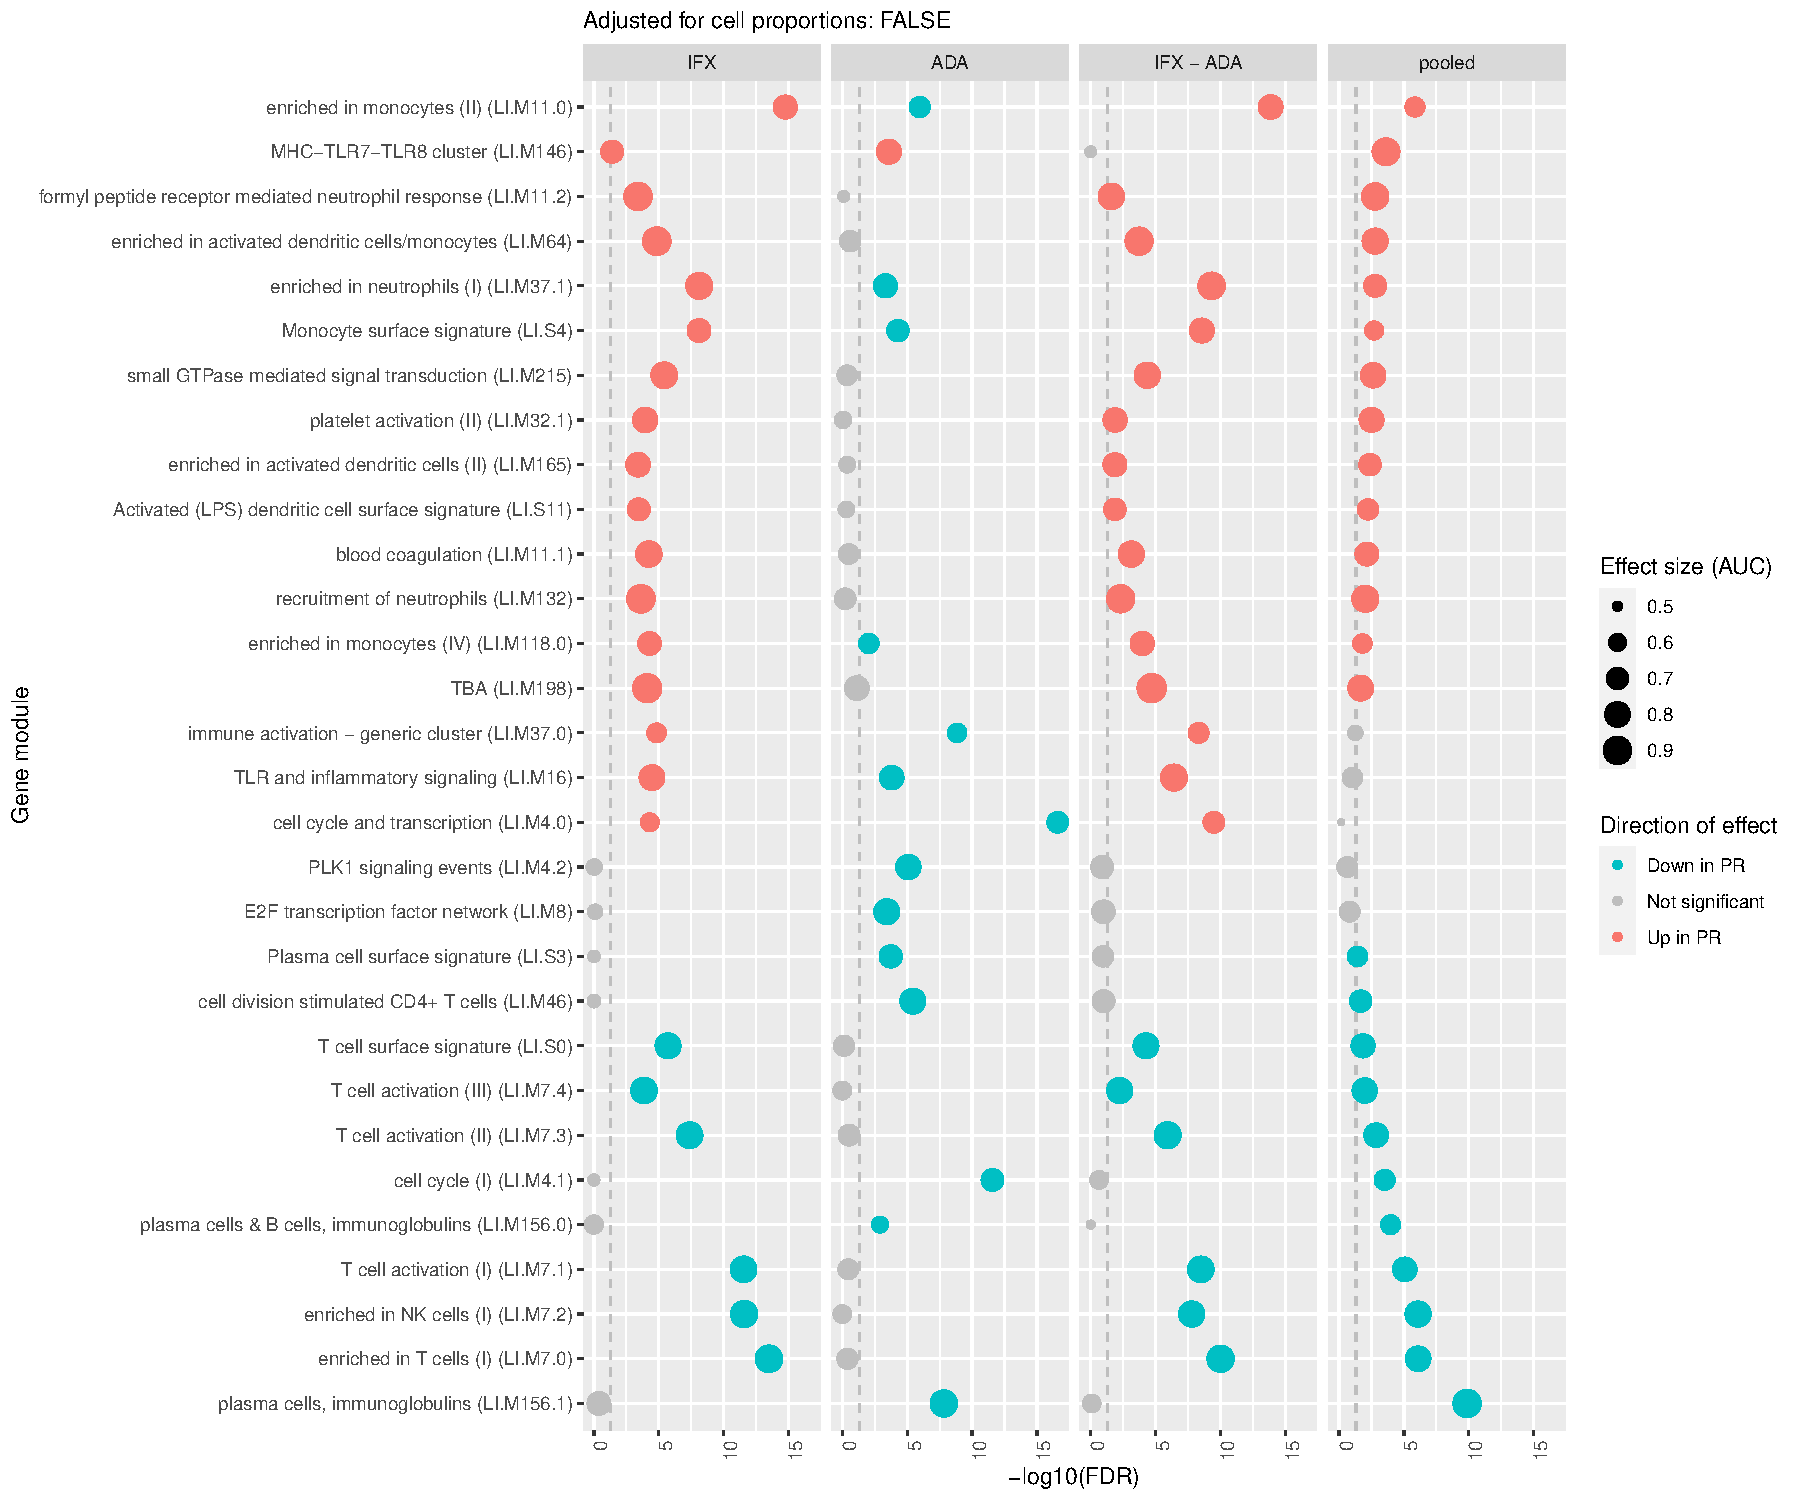
\includegraphics[width=1.0\textwidth,page=1]{mainmatter/figures/chapter_04/plot_gene_set_enrichment.tmodCERNO_panelplot_reversed_C_1RI_1NI,C_1RA_1NA,C_(1RI_1NI)_(1RA_1NA),C_1R_1N.cell_prop_correction_FALSE.pdf}
    \caption{Panel plot of module enrichent analysis for PR vs PNR at week 0. Length of bar is effect size, shade is FDR. Blue is upreg in R, red is downreg in R.}
    \label{fig:multipants_dge_panelPlot_week_0_R_N_cellPropF}
\end{figure}

\begin{figure}
    \centering
    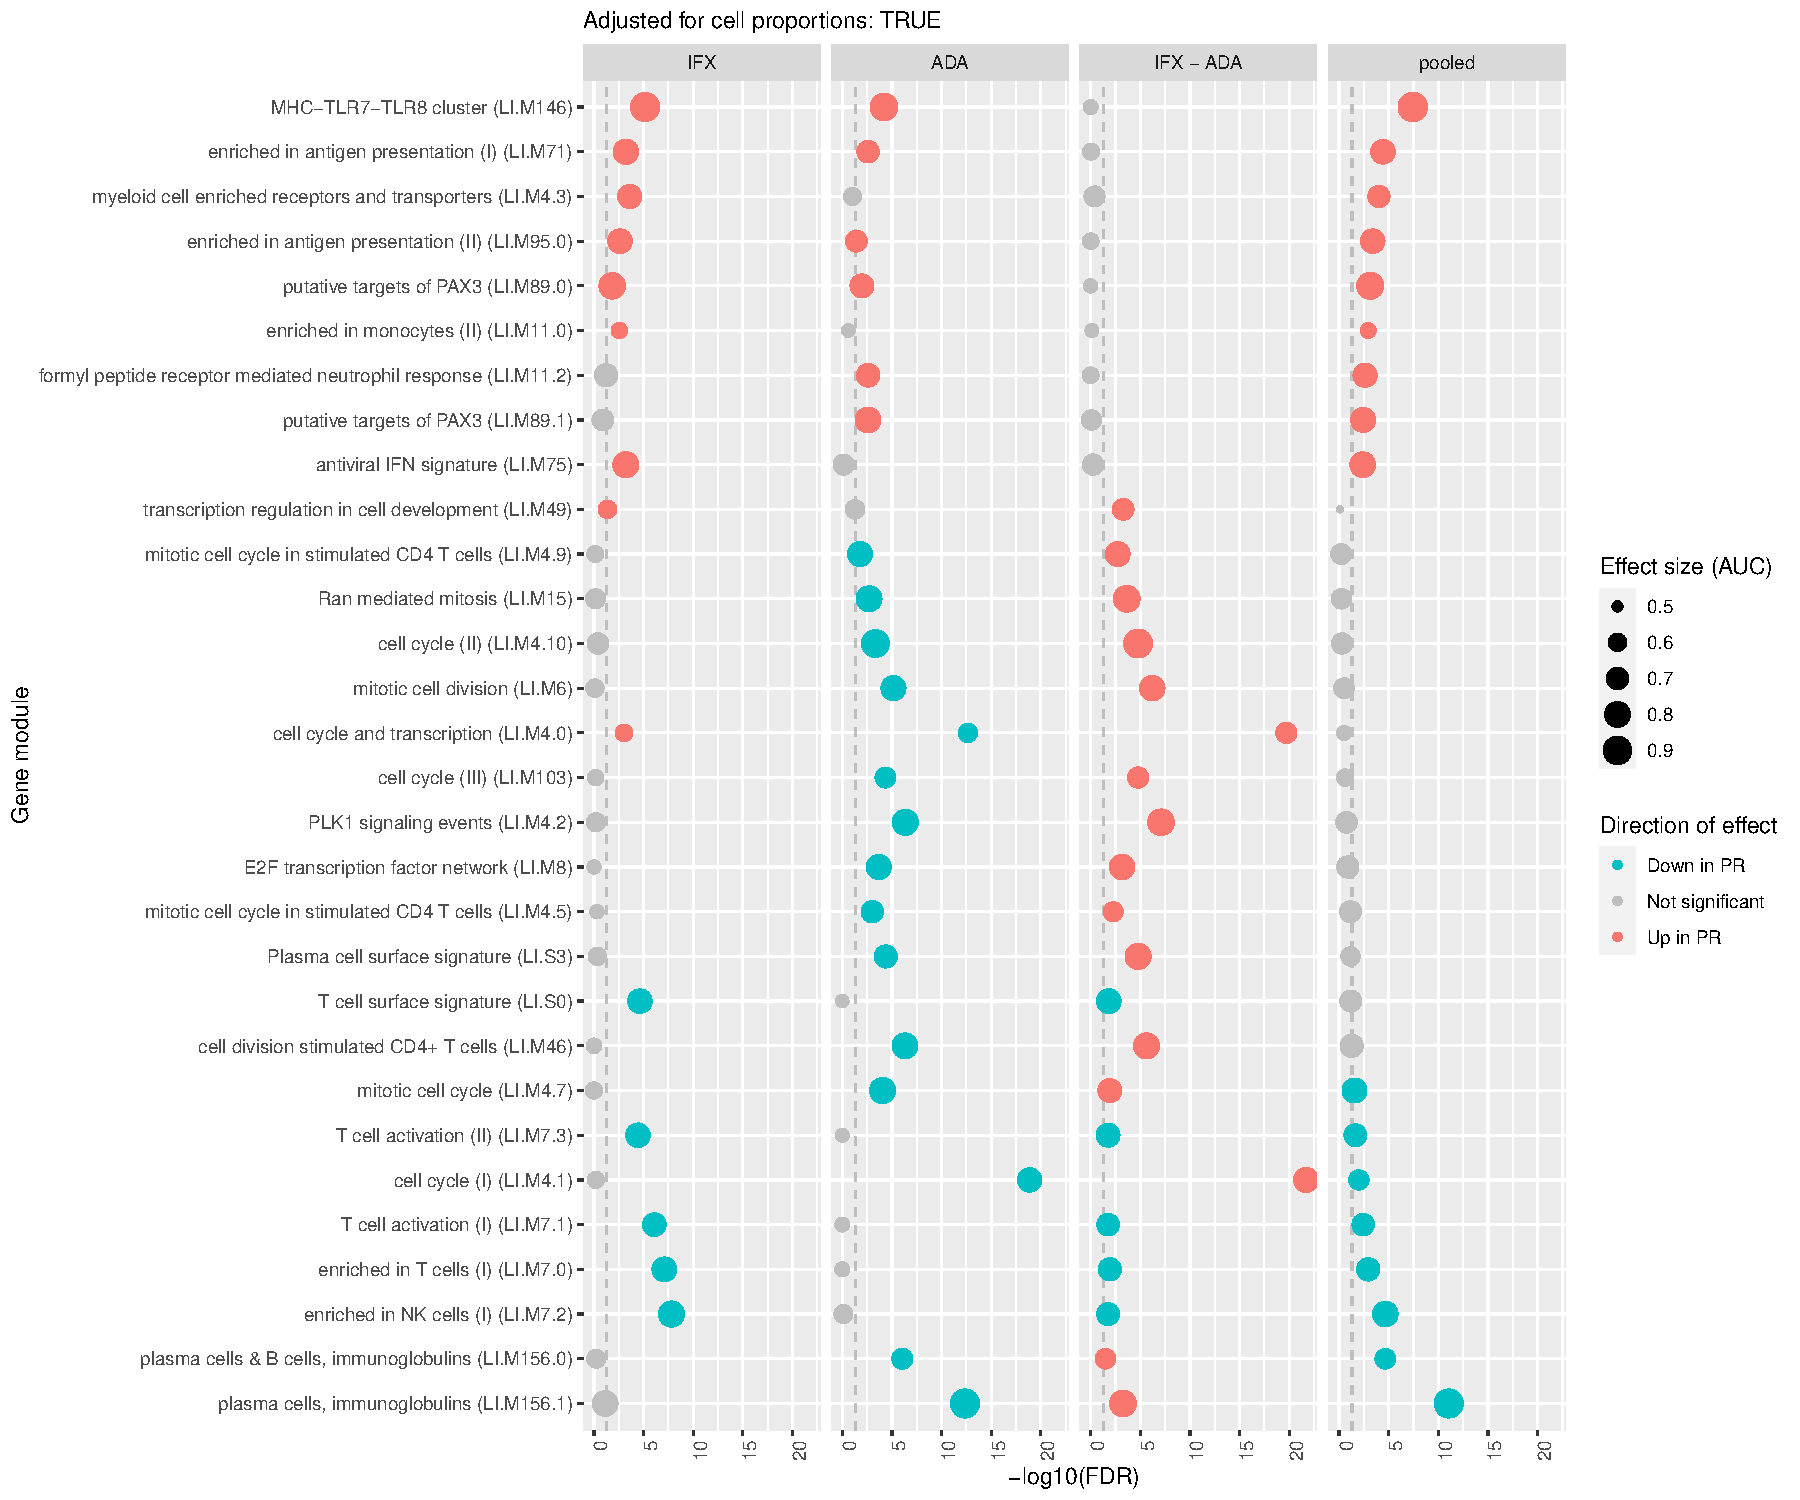
\includegraphics[width=1.0\textwidth,page=1]{mainmatter/figures/chapter_04/plot_gene_set_enrichment.tmodCERNO_panelplot_reversed_C_1RI_1NI,C_1RA_1NA,C_(1RI_1NI)_(1RA_1NA),C_1R_1N.cell_prop_correction_TRUE.pdf}
    \caption{Panel plot of module enrichent analysis for PR vs PNR at week 0. Length of bar is effect size, shade is FDR. Blue is upreg in R, red is downreg in R.}
    \label{fig:multipants_dge_panelPlot_week_0_R_N_cellPropT}
\end{figure}

\subsection{Investigating previously reported baseline predictors of anti-\glsfmtshort{TNF} response in \glsfmtshort{PANTS}}

In addition to hits from this study, \autoref{fig:multipants_dge_volcano_week_0_R_N} is annotated with genes whose expression in gut biopsies or blood have been tested as baseline predictors of primary response in the literature\autocite{arijs2009MucosalGeneSignatures,arijs2010PredictiveValueEpithelial,verstockt2019LowTREM1Expression,salvador-martin2020GeneSignaturesEarly}.
Some genes expressed in gut mucosa (e.g. \gene{IL13RA2}) were not appreciably expressed in this whole blood dataset, 
and most other genes that were expressed were not differentially expressed.
Only \gene{TNFRSF1B} and \gene{PTGS2} were associated with primary response, specifically in the infliximab-only comparison unadjusted for cell composition.

A previously identified marker in blood \gene{TREM1}, found to have opposing in two studies from \autocite{gaujoux2019CellcentredMetaanalysisReveals,verstockt2019LowTREM1Expression}
was not significantly associated with response in this study
before (logFC=\num{0.29283535}, FDR=\num{0.0595323})
%      logFC  AveExpr          t    P.Value adj.P.Val      z.std
% 0.29283535 7.668094  2.8665957 0.00429233 0.0595323  2.8558388
or after adjusting for cell composition (logFC=\num{0.04625626}, FDR=\num{0.9864125}).
% 0.04625626 7.668094  0.6661333 0.50560221 0.9864125  0.6657010

% \begin{figure}
%     \centering
%     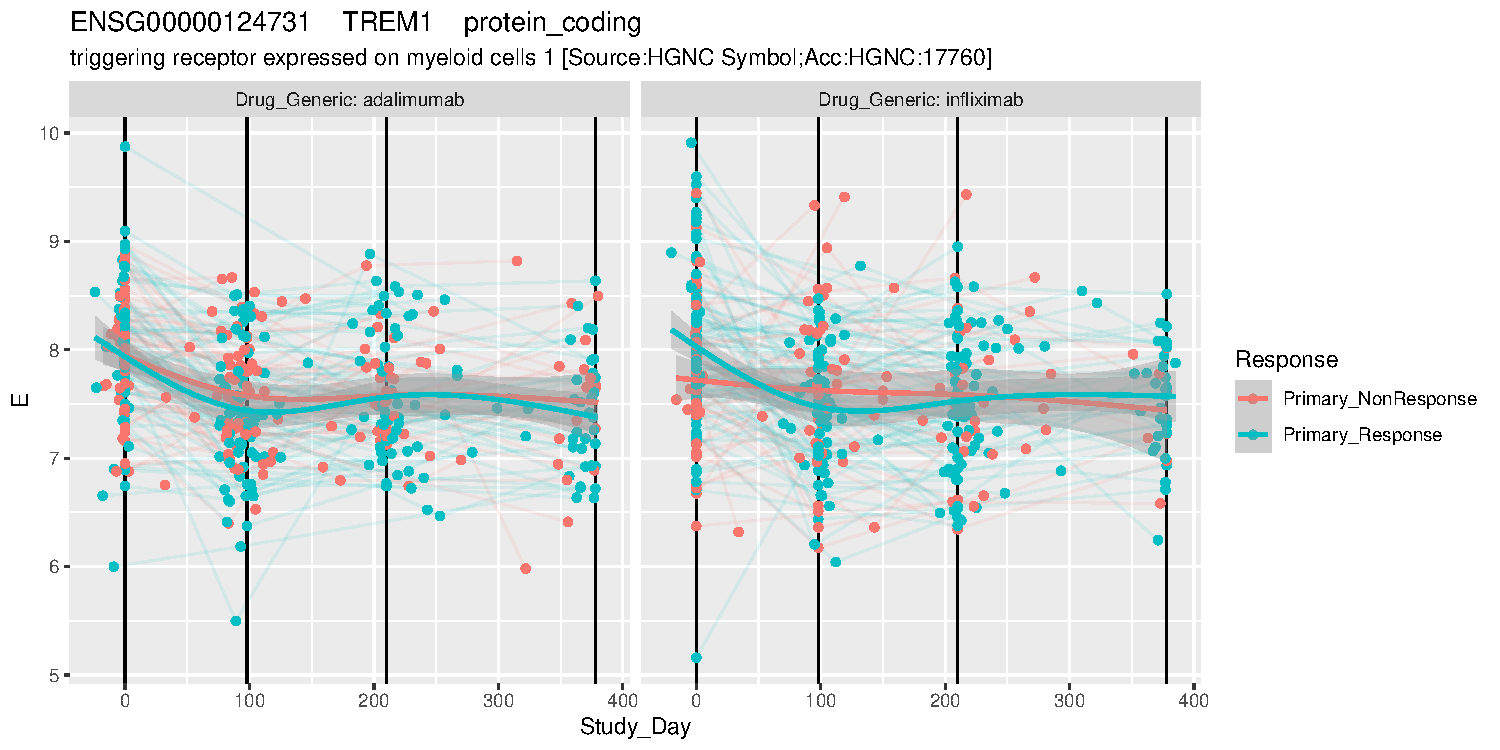
\includegraphics[width=1.0\textwidth,page=1]{mainmatter/figures/chapter_04/dream.E_vs_Study_Day.GENEID_ENSG00000124731.SYMBOL_TREM1.pdf}
%     \caption{Unadjusted, normalised TREM1 expression over time}
%     \label{fig:multipants_dge_TREM1}
% \end{figure}

\subsection{Gene expression associated with primary response after anti-\glsfmtshort{TNF} induction}

The same methodology applied at week 0 was applied at week 14 to identify differences in post-induction expression associated with primary response.
A larger proportion of the transcriptome is differentially expressed at week 14: 
1364 for the infliximab-only comparison, 
1544 for the adalimumab-only comparison, 
and 4841 pooling both drugs (\autoref{fig:multipants_dge_volcano_week_14_R_N}).
No significant interactions between drug and primary response were detected at the gene-wise level.
Given that sample sizes at week 0 and week 14 are comparable (\autoref{fig:multipants_studyDay_boxplots}), the overall signal is much stronger than at baseline.

Adjusting for cell proportions, 1320/1367, 1515/1544 and 4653/4841 have dampened effects;
and the numbers of significant genes drop to 379, 177, and 1302 for infliximab, adalimumab, and pooled analyses respectively.
This again suggests many effects are mediated by differences in immune cell composition between primary responders and non-responders.

Modules including generic immune activation, monocytes, TLR and inflammatory signalling, and neutrophils were downregulated in primary responders; 
whereas B cell and plasma cell modules were upregulated \autoref{fig:multipants_dge_panelPlot_week_14_R_N_cellPropF}.
These modules remained differentially expressed with the same direction of effect after adjusting for cell composition \autoref{fig:multipants_dge_panelPlot_week_14_R_N_cellPropF}, 
suggesting there is per-cell up or downregulation on top of abundance changes of the cell types expressing these modules.
Directions of effect for the most significant modules were largely consistent between drugs, with little evidence for interactions at the module level.

\gene{SIGLEC10} from my baseline analysis retains its significant association with primary response post-induction, with the same direction of effect (adjusted logFC=\num{0.36610032}).
\todo{highlight a few more individual genes specific to this analysis too? not sure how to pick them at the moment.}
Some genes previously proposed as baseline markers of response in gut mucosa: \gene{G0S2}, \gene{TNFAIP6}, \gene{S100A8} and \gene{S100A9} by \autocite{arijs2010PredictiveValueEpithelial}; and \gene{OSM} by \autocite{west2017OncostatinDrivesIntestinal},
were differentially expressed in post-induction blood in this study.
The direction of effect in both cases, downregulation of markers in primary responders, also matches this study.

\begin{figure}
    \centering
    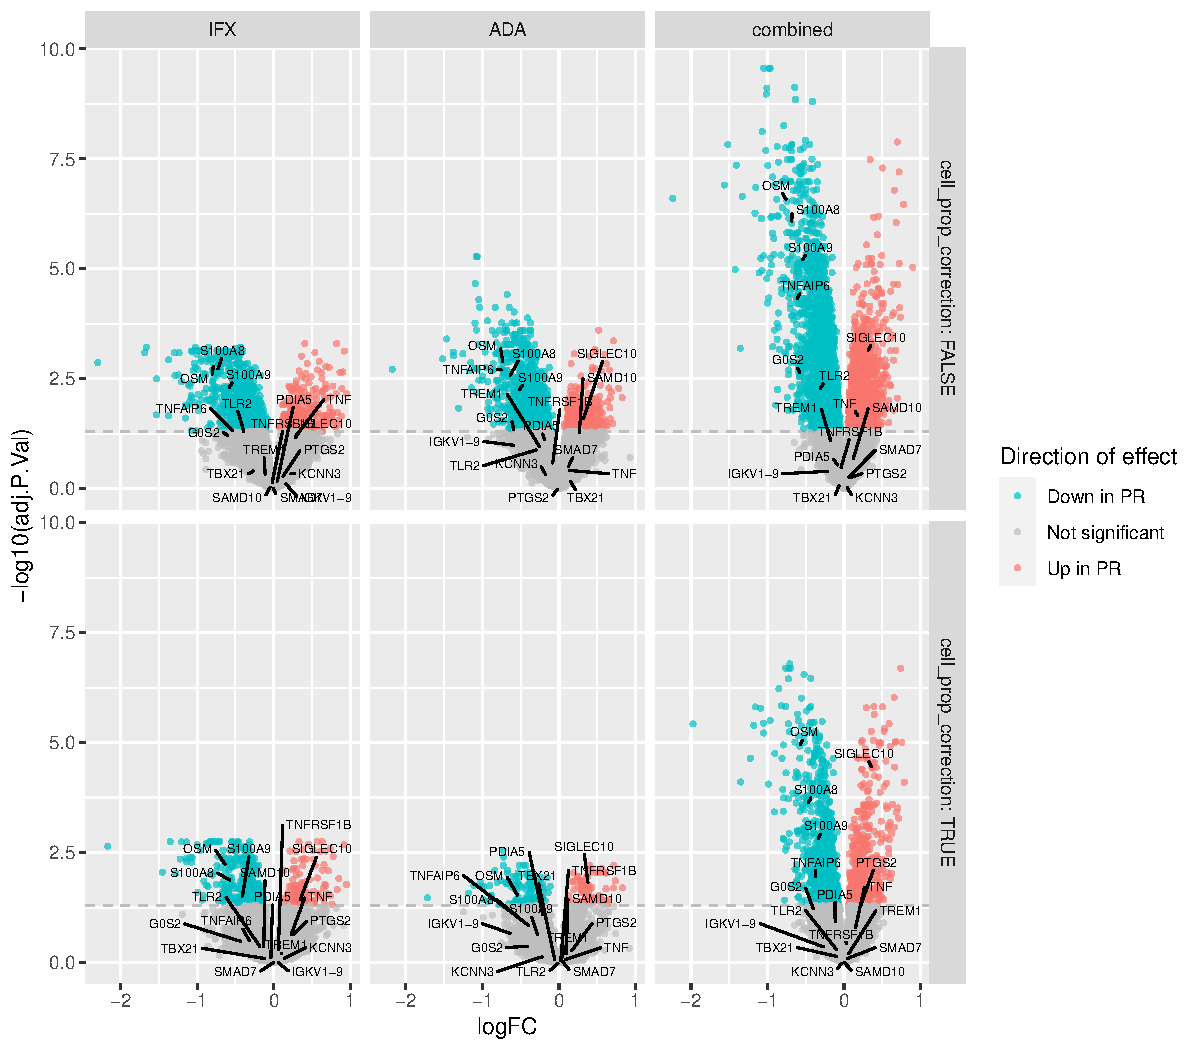
\includegraphics[width=1.0\textwidth,page=1]{mainmatter/figures/chapter_04/plot_gene_set_enrichment.dge_result_volcano_simple_C_3RI_3NI,C_3RA_3NA,C_3R_3N.pdf}
    \caption{DGE volcano plot for PR vs PNR at week 14}
    \label{fig:multipants_dge_volcano_week_14_R_N}
\end{figure}

\begin{figure}
    \centering
    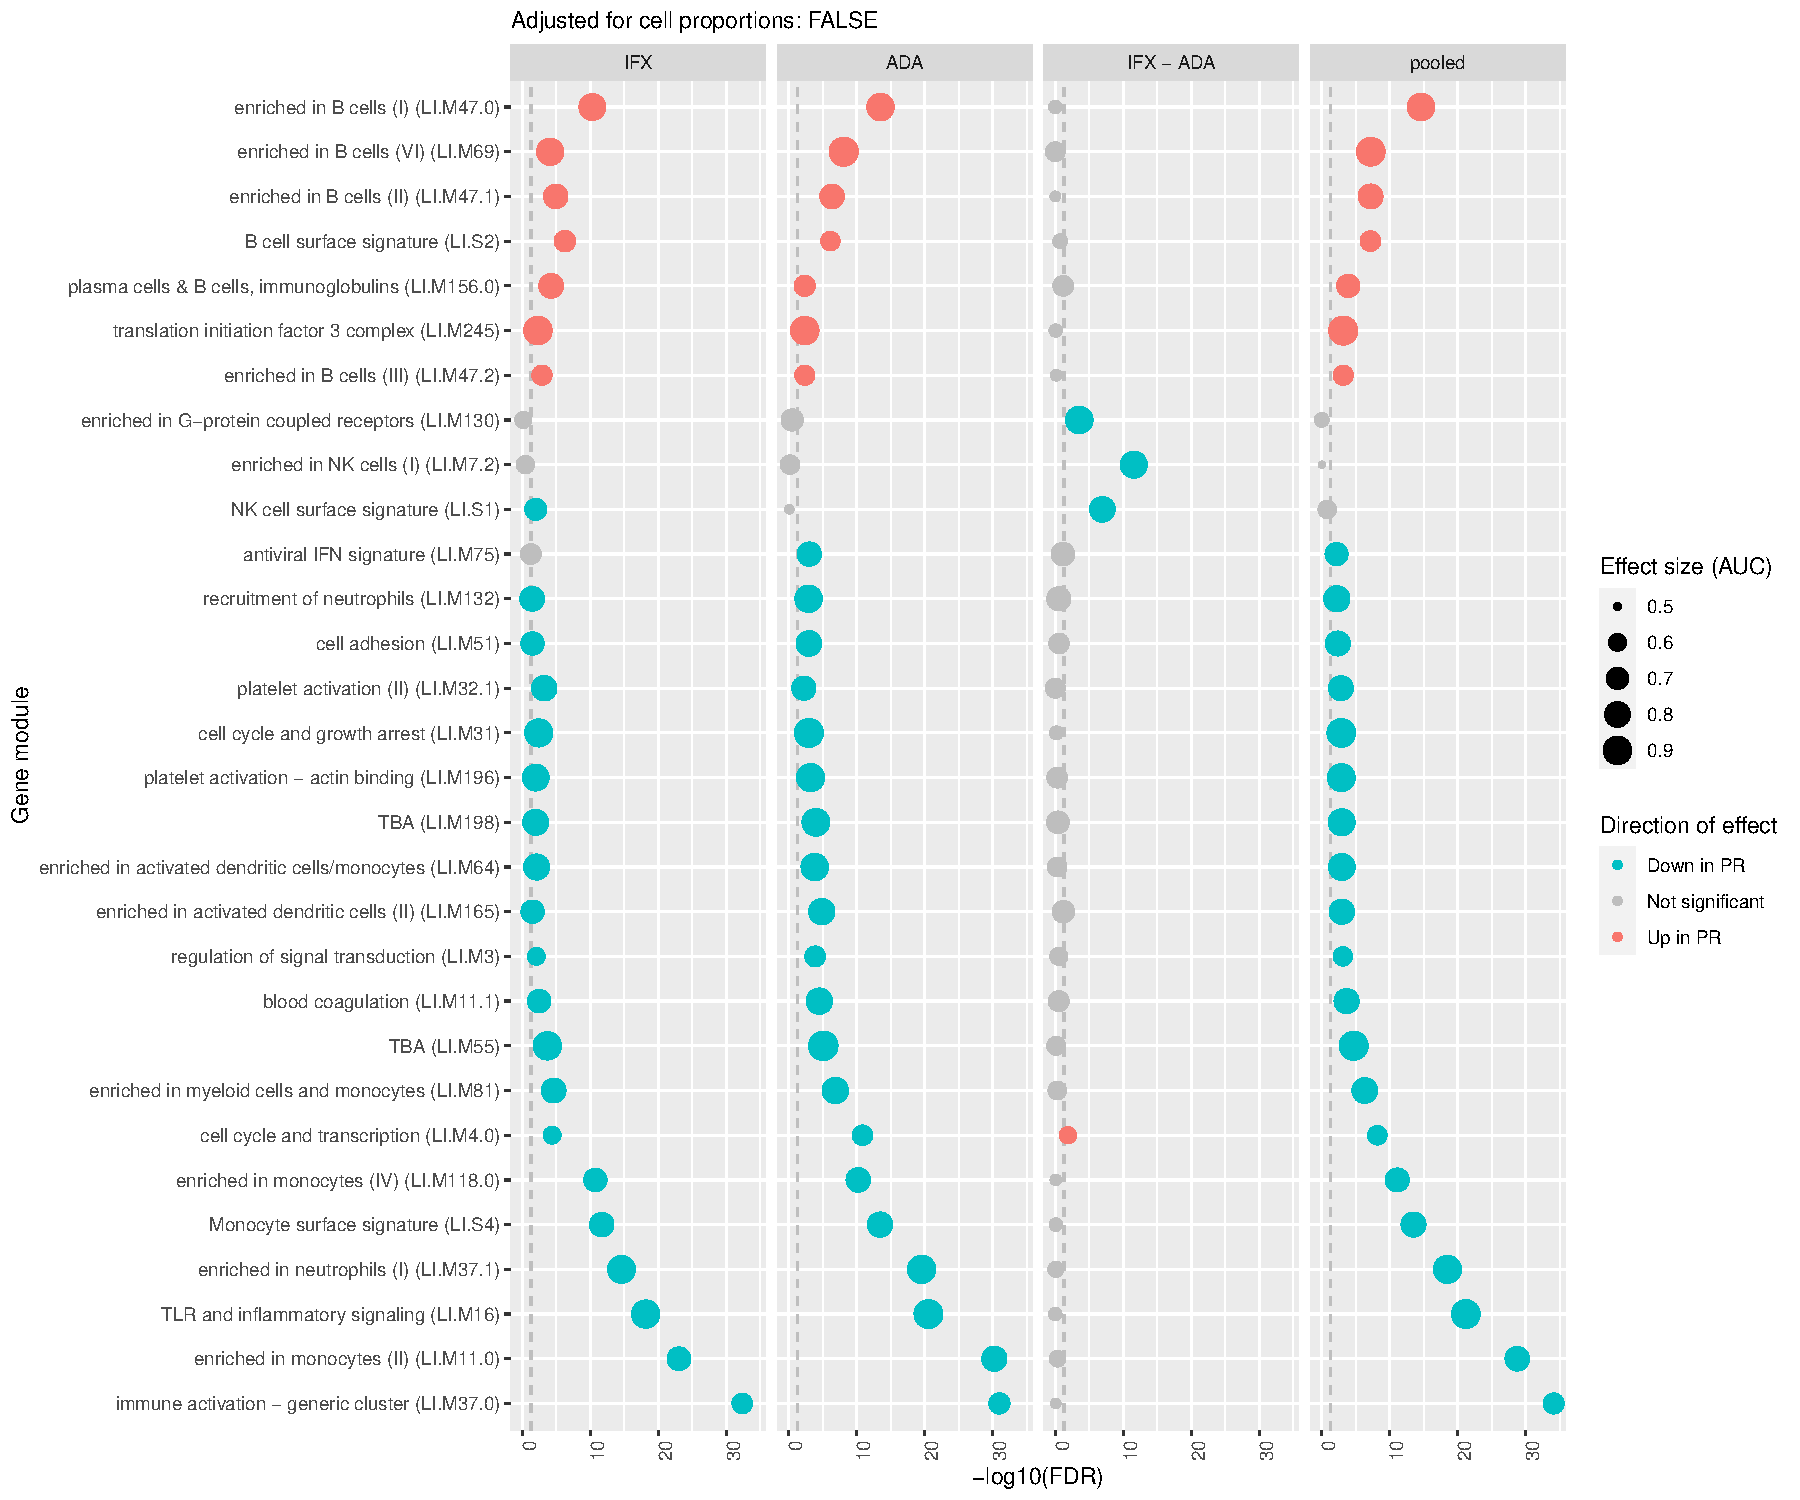
\includegraphics[width=1.0\textwidth,page=1]{mainmatter/figures/chapter_04/plot_gene_set_enrichment.tmodCERNO_panelplot_reversed_C_3RI_3NI,C_3RA_3NA,C_(3RI_3NI)_(3RA_3NA),C_3R_3N.cell_prop_correction_FALSE.pdf}
    \caption{Panel plot of module enrichent analysis for PR vs PNR at week 14, adjusted for cell comp. Length of bar is effect size, shade is FDR. Blue is upreg in R, red is downreg in R. top 20 by max}
    \label{fig:multipants_dge_panelPlot_week_14_R_N_cellPropF}
\end{figure}

\begin{figure}
    \centering
    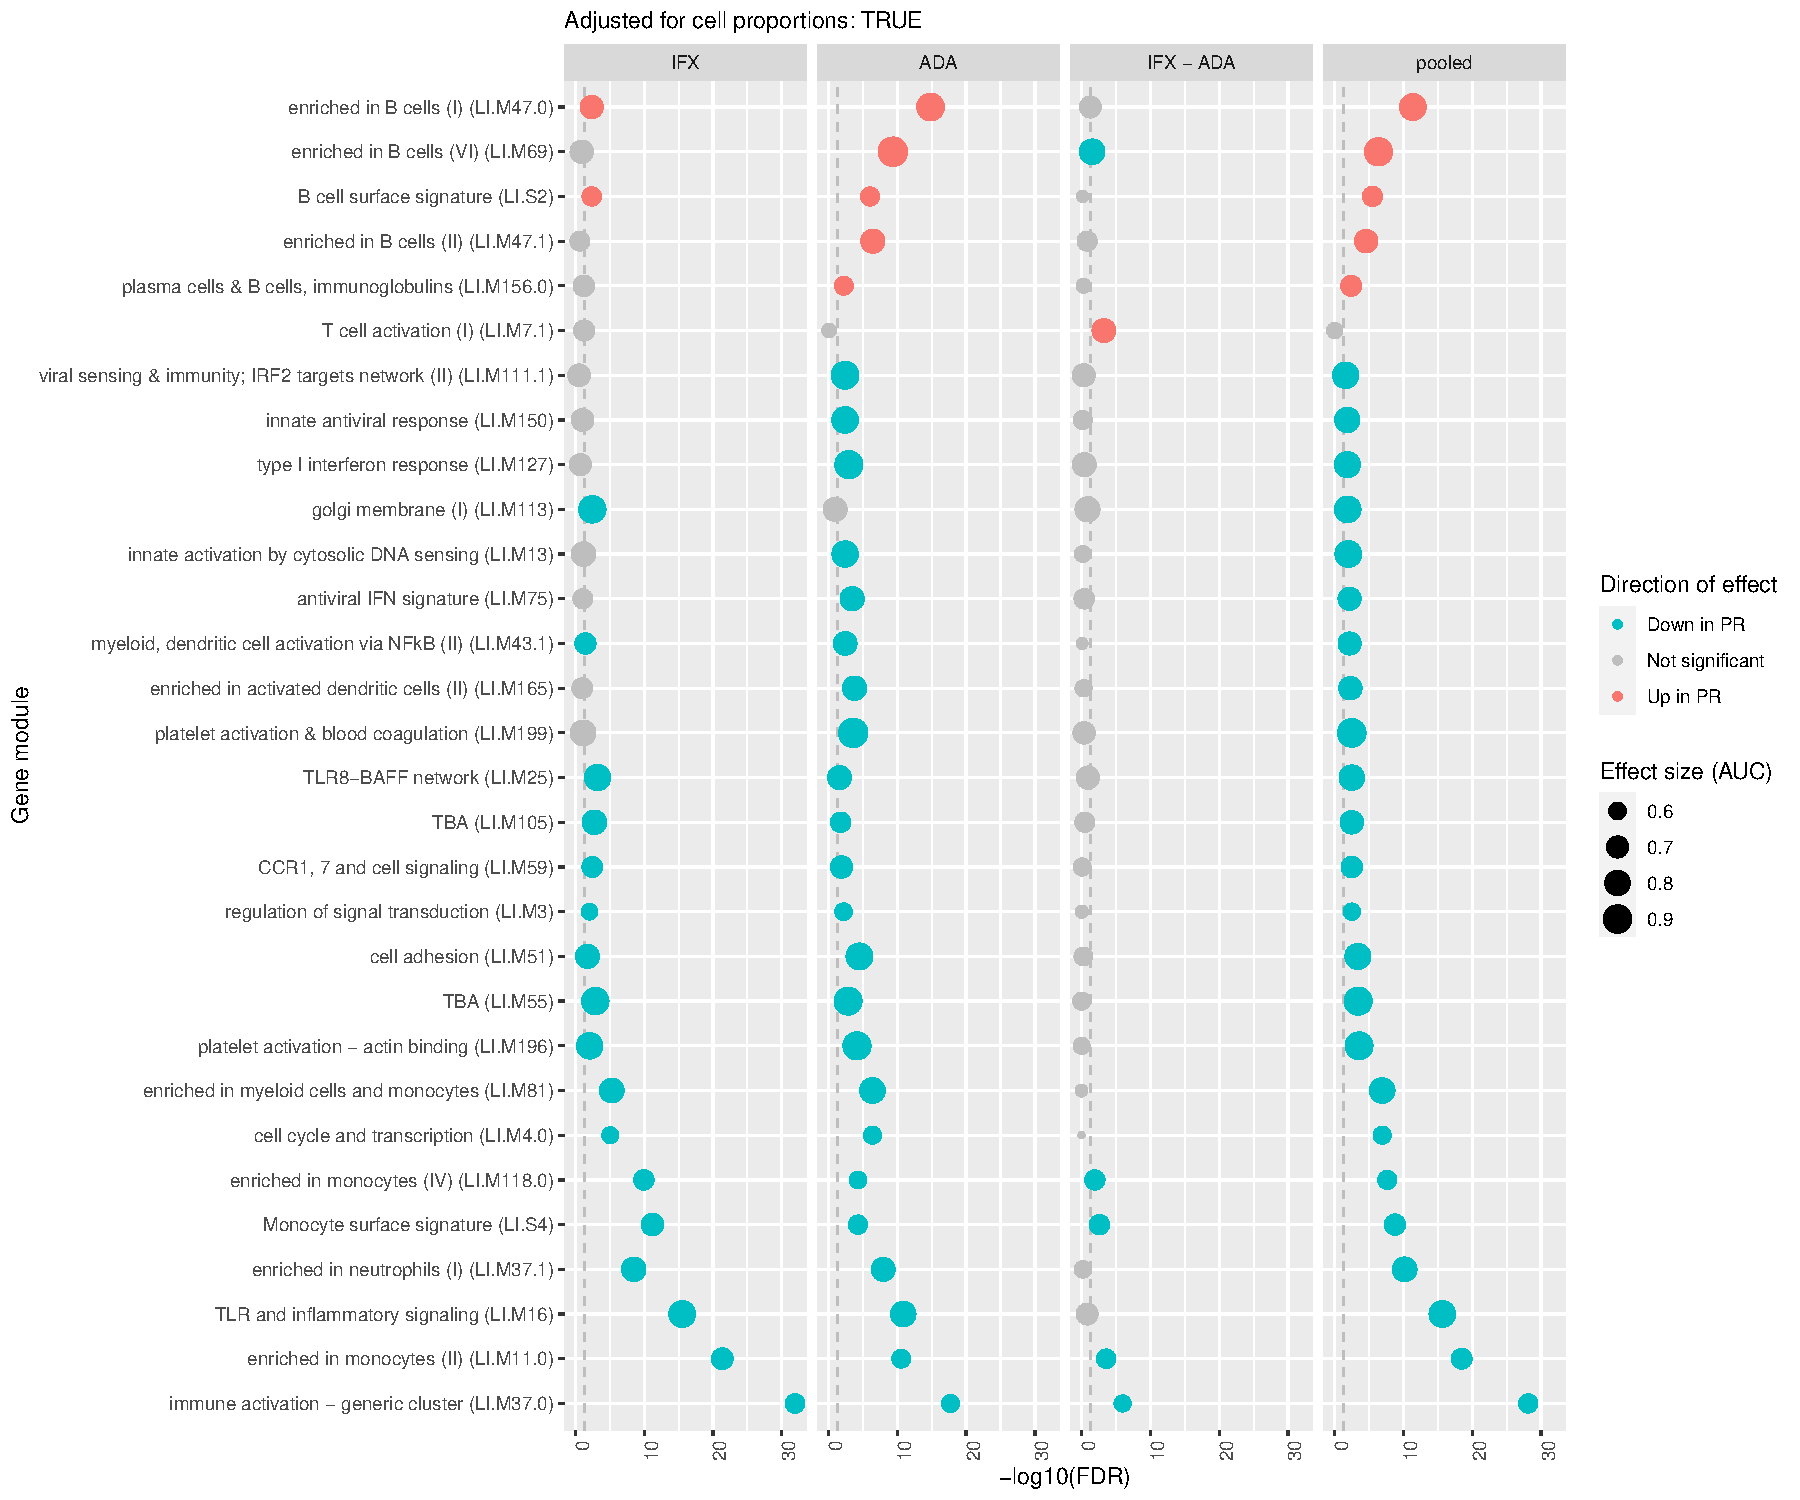
\includegraphics[width=1.0\textwidth,page=1]{mainmatter/figures/chapter_04/plot_gene_set_enrichment.tmodCERNO_panelplot_reversed_C_3RI_3NI,C_3RA_3NA,C_(3RI_3NI)_(3RA_3NA),C_3R_3N.cell_prop_correction_TRUE.pdf}
    \caption{Panel plot of module enrichent analysis for PR vs PNR at week 14, adjusted for cell comp. Length of bar is effect size, shade is FDR. Blue is upreg in R, red is downreg in R. top 20 by max}
    \label{fig:multipants_dge_panelPlot_week_14_R_N_cellPropT}
\end{figure}

\subsection{Changes in expression from baseline to post-induction are magnified in primary responders}

Given the stronger differences in expression between primary responders and non-responders at week 14 versus week 0,
I estimated the change in expression from week 0 to week 14 within the two groups, and also estimated the timepoint by response interaction.
This analysis was only done with drugs pooled, as it was concluded in previous sections that power to assess three-way interactions in this dataset may be limited.

Without adjusting for cell proportions, 
12862 genes were differentially expressed in primary responders at week 14 vs week 0,
8310 genes in primary non-responders,
and 6320 genes had a significant interaction;
after adjusting for cell proportions, 
5572 genes were differentially expressed in primary responders,
626 genes in primary non-responders,
and 179 genes had a significant interaction.

Of the genes differentially expressed between week 14 and week 0 in both primary responders and non-responders,
and with a significant interaction between timepoint and response, 
nearly all (4885/4891 unadjusted for cell composition, 31/32 adjusted) were magnified by primary response,
such that the same genes have larger fold-changes in the same direction for primary responders (\autoref{fig:multipants_dge_logFC_C_3R_1R_vs_logFC_C_3N_1N}).

% TODO: am here: modules that change same in R and NR, but more signif in R
The modules that change from week 0 to week 14 in 
These are many of the same modules that are differentially expressed between primary responders and non-responders at week 14.

% TODO Some exceptions for flipped effects

% \begin{figure}
%     \centering
%     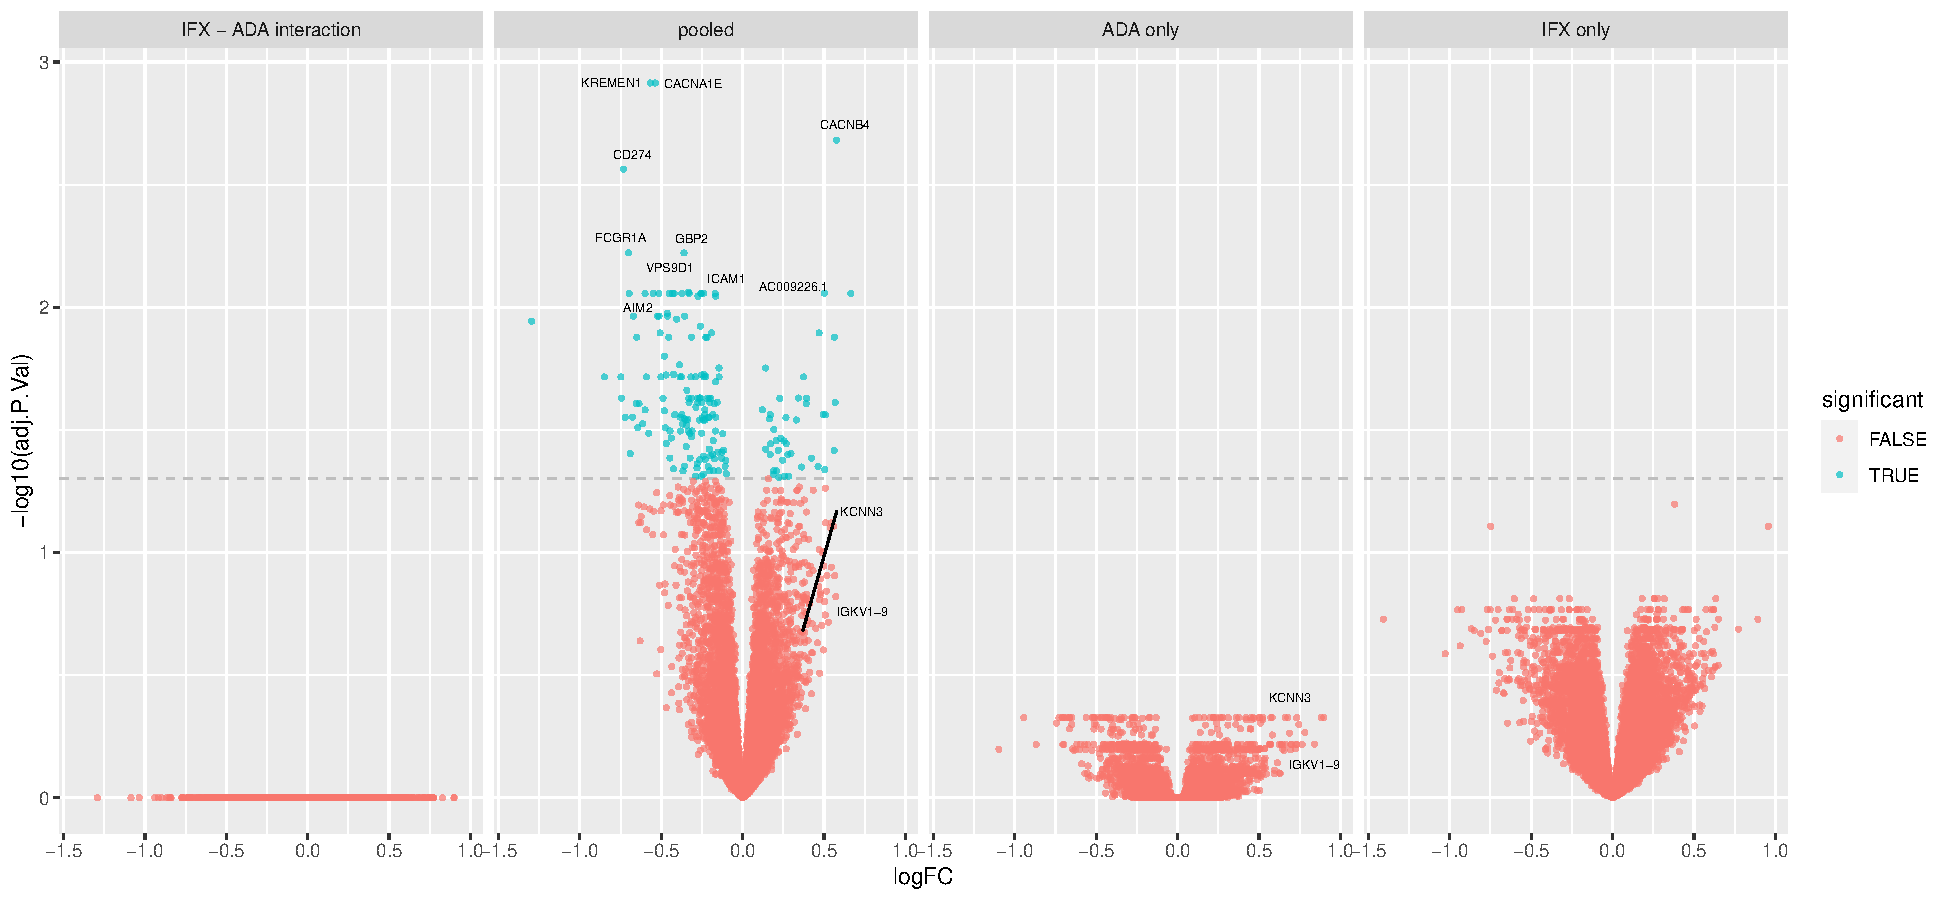
\includegraphics[width=1.0\textwidth,page=1]{mainmatter/figures/chapter_04/plot_gene_set_enrichment.dge_result_volcano_C_(3RI_1RI)_(3NI_1NI),C_(3RA_1RA)_(3NA_1NA),C_((3RI_1RI)_(3NI_1NI))_((3RA_1RA)_(3NA_1NA)),C_(3R_1R)_(3N_1N).pdf}
%     \caption{DGE volcano plot for PR vs PNR for week 14 - week 0 change}
%     \label{fig:multipants_dge_volcano_week_14_0_R_N}
% \end{figure}
%
% \begin{figure}
%     \centering
%     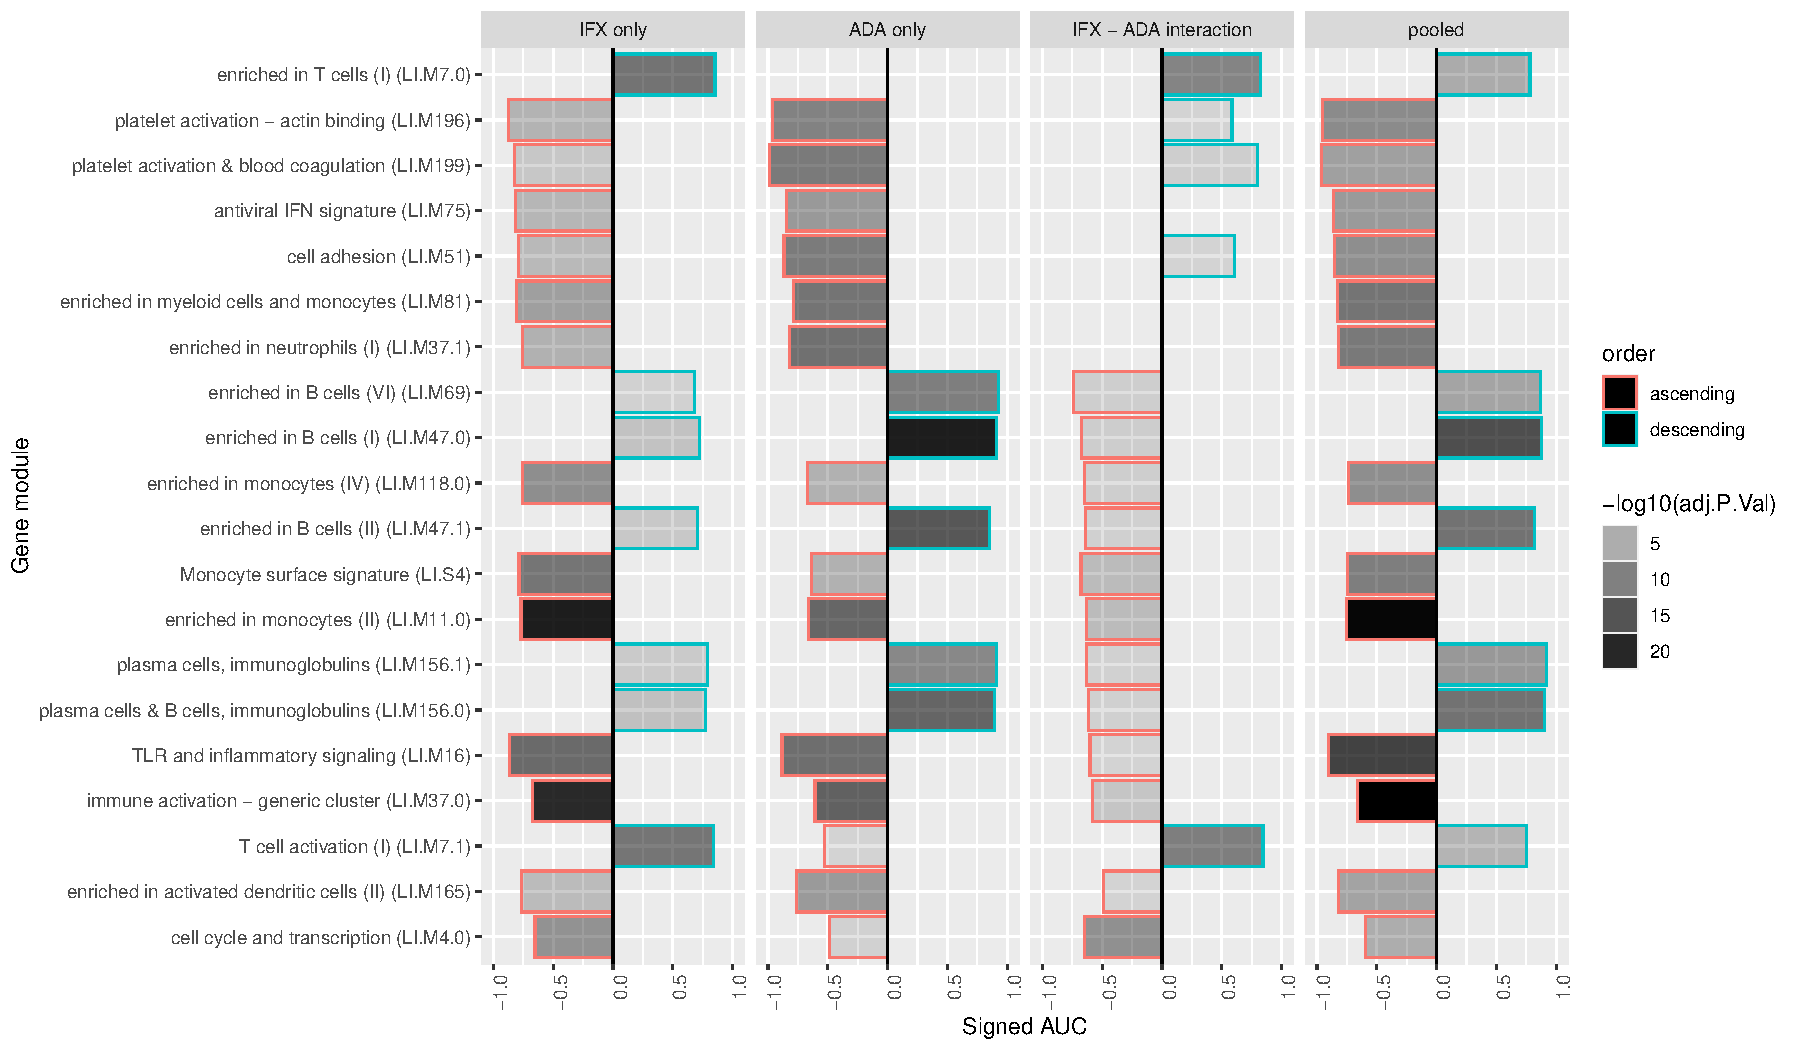
\includegraphics[width=1.0\textwidth,page=1]{mainmatter/figures/chapter_04/plot_gene_set_enrichment.tmodCERNO_panelplot_C_(3RI_1RI)_(3NI_1NI),C_(3RA_1RA)_(3NA_1NA),C_((3RI_1RI)_(3NI_1NI))_((3RA_1RA)_(3NA_1NA)),C_(3R_1R)_(3N_1N).pdf}
%     \caption{Panel plot of module enrichent analysis for PR vs PNR for week 14 - week 0 change. Length of bar is effect size, shade is FDR. Blue is upreg in R, red is downreg in R.}
%     \label{fig:multipants_dge_panelPlot_week_14_0_R_N}
% \end{figure}

\begin{figure}
    \centering
    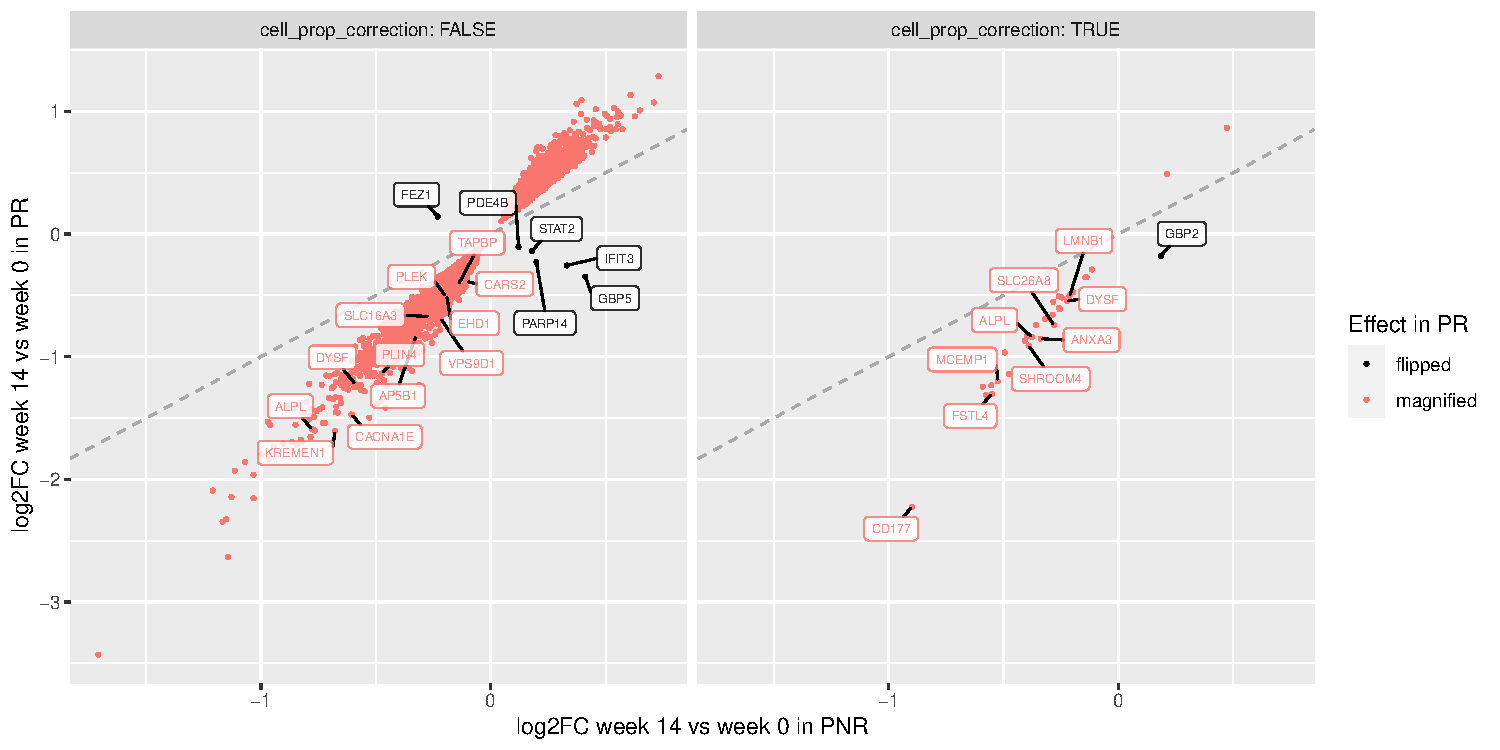
\includegraphics[width=1.0\textwidth,page=1]{mainmatter/figures/chapter_04/plot_gene_set_enrichment.logFC_C_3R_1R_vs_logFC_C_3N_1N.pdf}
    \caption{}
    \label{fig:multipants_dge_logFC_C_3R_1R_vs_logFC_C_3N_1N}
\end{figure}

\subsection{Sustained expression differences between primary responders and non-responders during anti-\gls{TNF} maintenance}

% "This is an observational study and the clinician may decide to continue with anti-TNF therapy even if the patient meets the study definition of primary non-response."
\1 despite pnr at w14, some patients continue
\1 Finally, spline model as a formal way to test general differences between PR and PNR over all timepoints
    \2 instead of doing every pairwise R vs NR comparison
    \2 266 hits at FDR < 0.05
    \2 clustering the expression of spline hits finds two main patterns: upregulation and downregulation after starting anti-TNFs, magnified in responders (\autoref{fig:multipants_dge_spline1})
    \2 from this analysis, can additionally see that expression differences are maintained even out to week 54
    \2 most hits in the spline have already been found in the separate w0, w14 or w14-w10 R vs NR comparisons (only 81 unique), but confirms the maintain

pooled only, since lower numbers for later timepoints

\begin{figure}
    \centering
    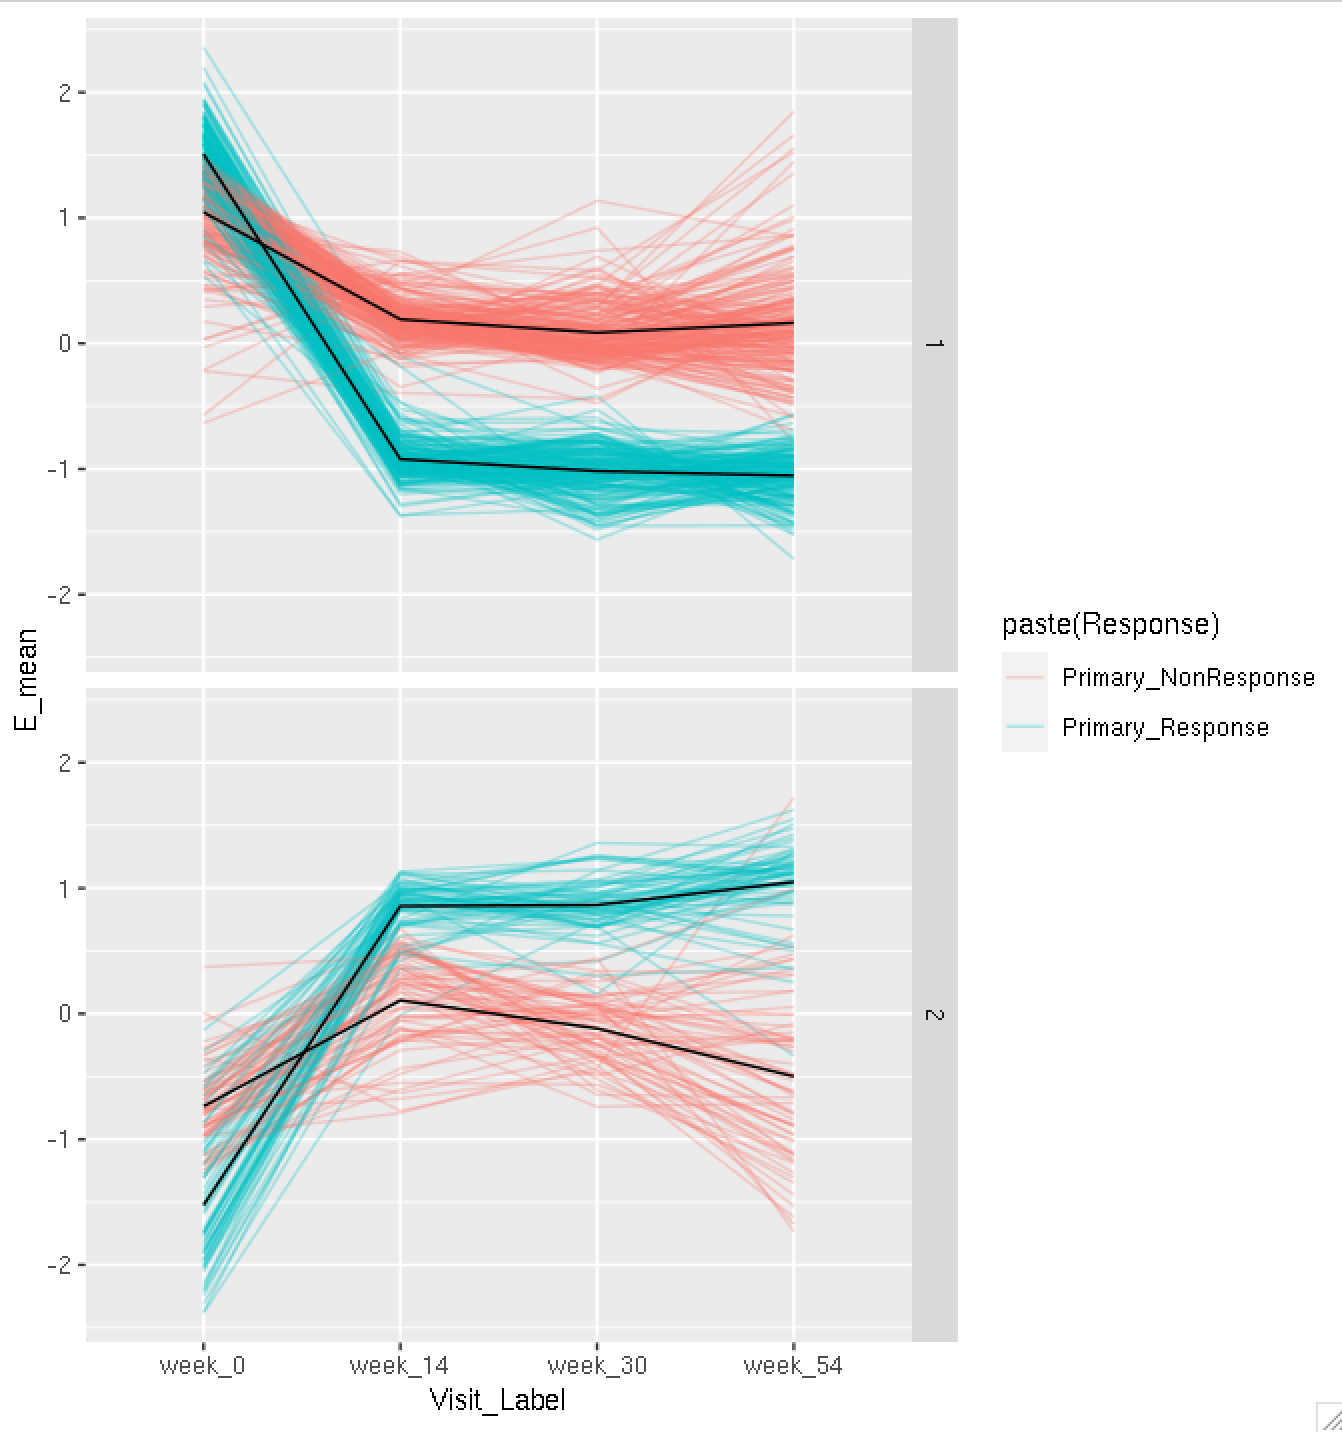
\includegraphics[width=1.0\textwidth,page=1]{mainmatter/figures/chapter_04/Screenshot 2020-08-06 at 16.09.43.png}
    \caption{Clustered expression over time for DGE genes in spline analysis}
    \label{fig:multipants_dge_spline1}
\end{figure}
    
\subsection{Genetics of gene expression over time}

\1 given the substantial changes in expression after starting the drug, are there differences in genetic control of expression of the course of taking the drug? \todo{have not put in an interaction between R and NR, not sure if powered}
\1 mapped eQTLs per timepoint, then did joint analysis with mashr
    \2 15040 genes tested after filtering
    \2 11156/15040 (0.74175531914) of genes are eGenes: have at least 1 eQTL in at least 1 timepoint (mashr lfsr < 0.05)
    \2 TODO: assess pc that are DGE
\1 based only on lfsr threshold, most eQTLs are shared: 999 significant in 1 timepoint, 381 significant in 2 timepoints, 526 significant in 3 timepoints, 9250 significant in all 4 timepoints
    \2 formal test: compared 3 post-drug timpoints with baseline: did test for difference of betas between w0 and w14, w0 and w30, w0 and w54 to identify reQTLs with difference in effects while avoid thresholding effects
    \2 only 6 hits at BH FDR < 0.05. Strongest effects at w0 vs w54: five of the six are for w0 vs w54 (\autoref{fig:multipants_reQTL_pm_w30_vs_w0_and_w54_vs_w0})

\begin{figure}
    \centering
    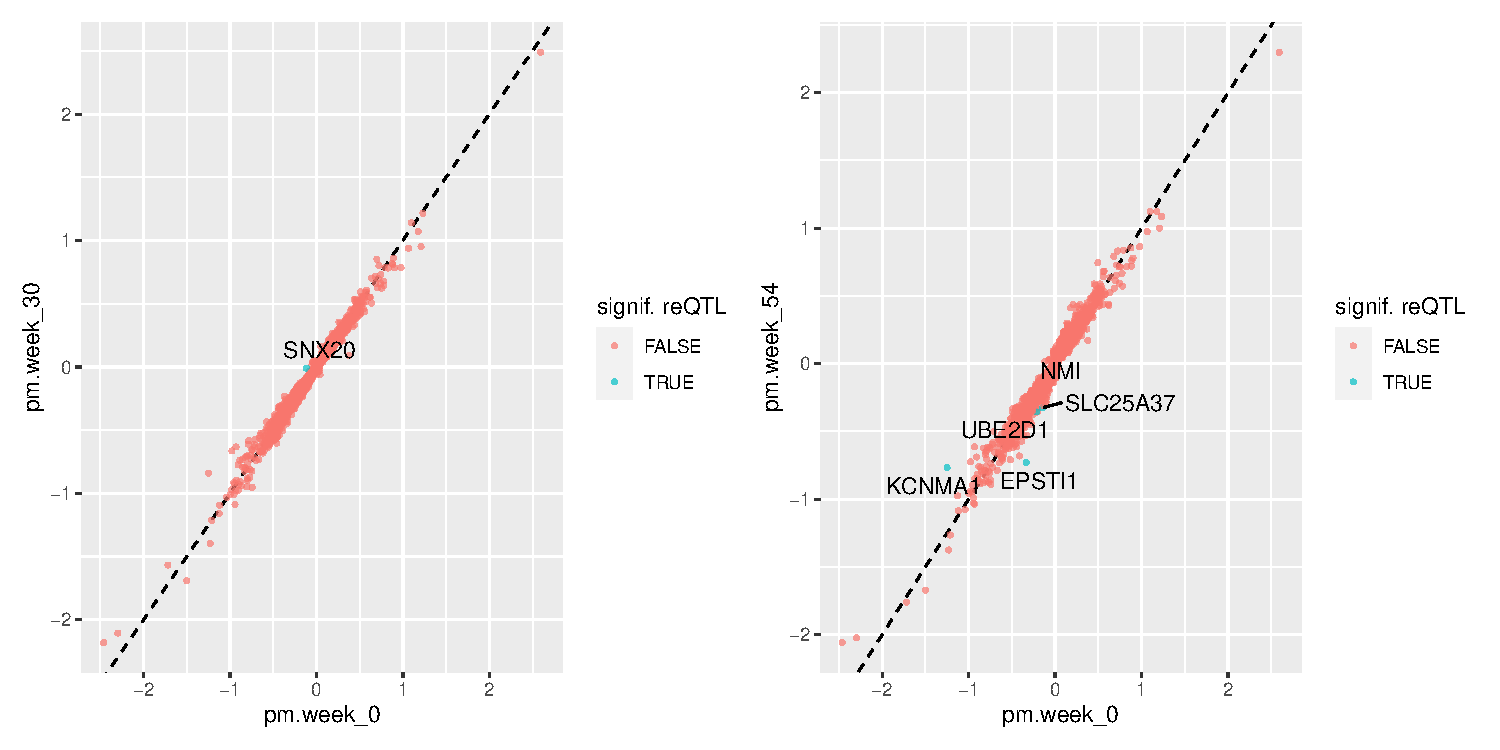
\includegraphics[width=1.0\textwidth,page=1]{mainmatter/figures/chapter_04/plot_dge_eqtl.pm_w30_vs_w0_and_w54_vs_w0}
    \caption{Week 30 and week 54 eQTL effect sizes vs baseline. Significant reQTLs in blue.}
    \label{fig:multipants_reQTL_pm_w30_vs_w0_and_w54_vs_w0}
\end{figure}

\1 clustering of eQTL effect sizes across 4 timepoints to identify general patterns of change in beta \todo{similar to the idea of moving from single gene to gene set analyses for more sensitivity}
    \2 start with prefilter for any reQTL significant at nominal p < 0.05. There were 344.
        \3 327/344 significant in all timepoints, so align ok
    \2 3 main clusters: high effect at w54, high effect at w0 and intermediate cluster (\autoref{fig:multipants_reQTL_clusters}) \todo{check if ADCY3 is in cluster 3}
    \2 GSEA on cluster 1 revealed enrichment of genes with interferon regulatory motifs in cluster 1 (\autoref{fig:multipants_reQTL_clusters_gprofiler})
    \2 2 INF genes
    % NMI EPSTI1
    
\begin{figure}
    \centering
    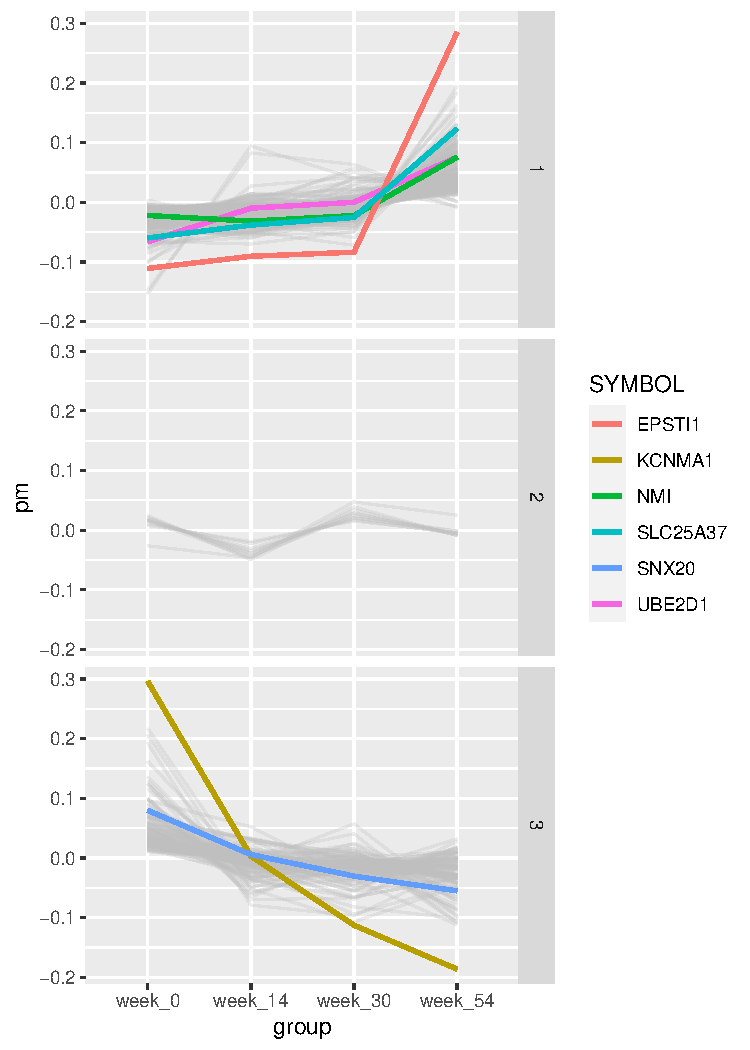
\includegraphics[width=1.0\textwidth,page=1]{mainmatter/figures/chapter_04/plot_dge_eqtl.reQTL_clusters.pdf}
    \caption{Clustering of eQTL betas over the 4 visits}
    \label{fig:multipants_reQTL_clusters}
\end{figure}

\begin{figure}
    \centering
    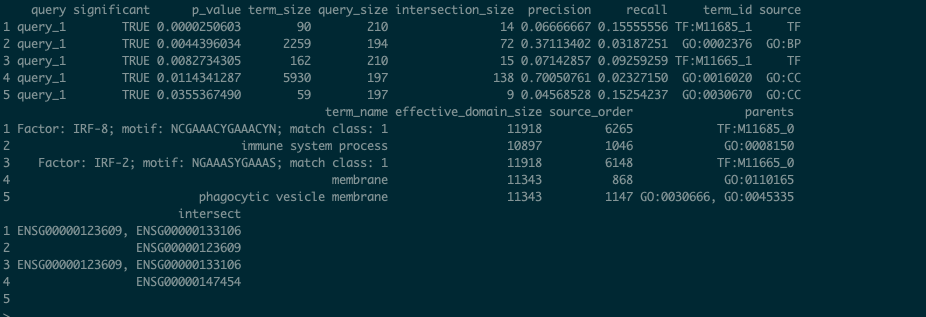
\includegraphics[width=1.0\textwidth,page=1]{mainmatter/figures/chapter_04/Screenshot 2020-08-12 at 21.50.28.png}
    \caption{gene set enrichment using gprofileR for cluster 1 genes}
    \label{fig:multipants_reQTL_clusters_gprofiler}
\end{figure}

\section{Discussion}

\1 <study summary>
    \2 in PANTS, a date cohort of anti-TNF naive CD patients who then got ADA/IFX with RNAseq in blood
    % at least pre splitting
    \2 measured gene expression differences between PR and PNR over 4 timepoints from 0 to 54 weeks
    \2 reQTL mapping to identify changes in genetic control of expression over the timepoints

\1 at week 14, difference in transcriptome between R/NR very distinct
    \2 generally more consistent between drugs
        \3 e.g. ADA-specific B cell downreg in PR effect seems to vanish in the tmod results at week 14
    \2 top hit KREMEN1 is part of an inflammatory apoptotic pathway \url{https://academic.oup.com/ibdjournal/article/14/suppl_1/S4/4653822}, makes sense that it is downreg in responders
    \2 modules: innate (monocyte/TLR and inflam) down in R. makes sense
        % \3 TODO: monocytes as previous markers?
        % \2 using classical / nc markers
    \2 modules: T and B cells up in R \todo{why???}

\1 at baseline, SIGLEC10 and CROCC2 were significantly upregulated in future PR to anti-TNF in the pooled analysis, with concordant direction of effect in both drugs
% IFX: probably due to cell comp
% ADA: probably not only due to cell comp, or not completely adjusting
    \2 high levels of SIGLEC10 in nc-monocytes \url{https://jbiol.biomedcentral.com/articles/10.1186/jbiol206} 
        % but more formal test required for e.g. nc mono
        \3 nc monocytes have a role in many chronic inflam diseases \url{https://www.annualreviews.org/doi/full/10.1146/annurev-immunol-042617-053119#_i16} including CD \url{https://www.researchgate.net/profile/Siew-Cheng_Wong/publication/221723208_The_three_human_monocyte_subsets_Implications_for_health_and_disease/links/09e415101253562a3c000000.pdf}
    \2 SIGLEC10 is one of the innate immune cell-surface Ig superfamily that binds with CD24 and repress DAMP-mediated inflammation. \url{https://www.nature.com/articles/mi201614?draft=collection}
    \2 in the context of IBD: Levels of DAMPS are increased in IBD. 
        \3 chronic inflam -> tissue death -> release of small proinflam molecules called DAMPs \autocite{desouza2016ImmunopathogenesisIBDCurrent}
        \3 "Interestingly, faecal calprotectin, the most frequently used and most sensitive marker of IBD clinical activity, is a complex of S100A8–S100A9, two prototypical DAMPs" \url{https://www.nature.com/articles/mi201614?draft=collection} \autocite{desouza2016ImmunopathogenesisIBDCurrent}
        % Previous studies investigating the association between baseline markers of inflammation and anti-TNF response are conflicting.2,30 
        \2 from \autocite{kennedy2019PredictorsAntiTNFTreatment} "In our study, higher baseline markers of inflammation predicted lower drug concentrations at week 14, suggesting that higher inflammatory load might contribute to faster drug elimination."
        \2 proposed model: baseline high SIGLEC10 -> low DAMP levels -> low inflam -> (higher drug conc at w14) -> primary response
            \3 it is stressed that this is a hypothetical model, no way to suggest causality due to the model used, and this being an uncontrolled cohort study
\1 not much known about CROCC2 (aka AC104809.3), but it's expression is nc-monocyte specific \url{https://dice-database.org/genes/AC104809.3} \url{https://www.proteinatlas.org/ENSG00000226321-CROCC2}
    \2 potential source of multiomics data for potential validation is \autocite{imhann20191000IBDProjectMultiomics}, contains drug response phenotypes
    \2 also, validate using protome/serological data in PANTS, although there is a known disconnect between proteome and transcriptome
        % expect modules to be more robust, esp since only a handful of hits for some comparisoins
    % projection techniques into public datasets e.g. GIMATS paper, but blood expressoin datasets needed, % could use some RA ones https://journals.plos.org/plosone/article?id=10.1371/journal.pone.0033199

\1 there ADA-specific downreg of gene modules in PR, especially plasma cell and immunoglobulins
    \2 includes one of the 3 hits: IGKV1-9
    \2 B cell genes down -> ??? -> response to anti-TNF
        \3 consistent, as TNF is involved in T cell-dependent B-cell responses, so inhibiting it should lower B cell response \url{https://www.ncbi.nlm.nih.gov/pmc/articles/PMC6235207/}
    \2 \textcite{gaujoux2019CellcentredMetaanalysisReveals} find lower props of inflam macrophage and plasma cell in IFX responders in gut biopsy
    \todo{I have no idea why the effect is stronger in ADA}
    \2 also, could be due to cell props, as B cell prop used in model is not perfectly correlated with plasma cell freq (see ch3)
    \2 differences in baseline characteristics between drugs discussed later on in limitations

Down regulation of plasma cells, B cells and immunoglobulin modules: module-level results line up with the three gene-wise hits for the adalimumab-only analysis.
KCNN3 is annotated to plasma cell surface signature module (LI.S3).
The expression of both \gene{KCNN3} and \gene{PDIA5} are correlated with blood plasmablast frequencies\autocite{tsang2014GlobalAnalysesHuman}.
IGKV1-9 encodes the immunoglobulin light chain variable region, and plasma cells are the cell type that secrete immunoglobulins.

even after adjusting: The pooled analysis results at baseline thus be interpreted with caution that some are driven by one drug

Why in this data does it appear that infliximab primary response is more correlated with baseline cell proportions than adalimumab primary response?
Difficult to answer here, as due to lack of randomisation infliximab and adalimumab patients differ by more than just the \gls{TNF}.

\1 replication of known baseline signatures
    \2 TREM1 signal from \textcite{verstockt2019LowTREM1Expression} is not replicated in this study, n.s. and opposite direction of effect
    \2 TREM1 Direction of effect is upregulated in PR, opposite to \autocite{verstockt2019LowTREM1Expression}, consistent with \autocite{gaujoux2019CellcentredMetaanalysisReveals}
    \2 potential differences in clinical vs endoscopic endpoint between all 3 studies
        % trem1 is more classical monocyte https://bmcgenomics.biomedcentral.com/articles/10.1186/1471-2164-10-403
    \2 effect decreases when adding cell proportion covariates: perhaps TREM1 mainly a surrogate for (monocyte) cell props?
    \2 the replication is sensitive to covariates, end points, drug
        \3 e.g. \textcite{verstockt2019LowTREM1Expression} did not use any covariates (i.e. t test), so they report an unadjusted effect
    \2 an aside: just as I examined previously known biomarkers, I expect replication of SIGLEC10 and CROCC2 before putting much credence into them
    \2 osm, tnf, tnfr2 \autocite{verstockt2019LowTREM1Expression}: consistent not DGE in blood

\1 went from few differences at w0 to many differences at w14 between R and NR
    \2 looking at change from baseline to week 14 confirmed mostly magnifying effects in R
        \3 could this suggest that there is a continuum of response?
    \2 the ones that are not consistent: what are they and could they give insights?
    \2 spline analysis confirmed that the diff starting at w14 is maintained at w30 and w54
    \2 \autocite{kennedy2019PredictorsAntiTNFTreatment}: "Continuing standard dosing regimens after primary non-response was rarely helpful; only 14 (12·4\% [95\% CI 6·9–19·9]) of 113 patients entered remission by week 54."
        \3 may be reflected in the transcriptomics too
    \2 attrition or loss to followup bias for reqtl effect
        % https://pubmed.ncbi.nlm.nih.gov/22611167/

        % https://stats.stackexchange.com/questions/354279/can-a-linear-mixed-model-handle-missing-data-that-is-not-missing-at-random
        % As you say, linear mixed-effects (LME) models are assuming that any missing data are missing at random (MAR). A way to account for suspected violations of the MAR assumption of LME models is to use joint models. Under this framework, the longitudinal response and the survival probability are associated by jointly estimating a single likelihood function. Using a joint model, you can get an estimate of how much a possible difference in survival is affecting the longitudinal response and how much the fluctuations in the longitudinal response are associated with survival.

        % https://sphweb.bumc.bu.edu/otlt/MPH-Modules/EP/EP713_Bias/EP713_Bias3.html
        % As noted above, the enrollment of subjects will not bias a prospective cohort study, because the outcome has not yet occurred. Therefore, choice cannot be related to both exposure status and outcome status. However, retention of subjects may be differentially related to exposure and outcome, and this has a similar effect that can bias the results, causing either an overestimate or an underestimate of an association.
        % Again, depending on which category is underreported as a result of differential loss to follow-up, either an underestimate or overestimate of effect (association) can occur.

        % likely direction is conservative since the most NR usually withdraw??

\1 <more limitations: internal validity>

    \2 a key question for interpreting both the DGE and reQTL results is the definition of visit and study day
        \3 arguably, time is only meaningful wrt to drug naive/on drug, and time since last dose and to next dose i.e. everyone is at trough drug levels
        \3 real drug levels over time will be peaky % TODO: half life \autocite{tracey2008TumorNecrosisFactor,lichtenstein2013ComprehensiveReviewAntitumor}
        \3 I included LOR and EXIT visits based on a time window, but in reality, patients that have more LOR have 
        % "A LOR visit should be scheduled any time after week 14 if the LOR criteria are met (page 11) and the patient’s gastroenterologist has escalated steroid, immunomodulatory or anti-TNF therapy. Escalation of anti-TNF therapy includes an increase in the dose, or a shortening of the interval between doses."
        \3 It should be noted that one option following patient loss of response is dose escalation, so samples from the same patient \emph{after} recorded loss of response may actually represent a different trough drug level to the rest.
            % TODO: read Sim email
    \2    % drug_level adjustment
        \3 why R change E, but NR don't? faster clearance? adjust for drug level to see this
        \3 but I did not use trough drug level measured on or near the same study day as a covariate
        \3 this would explain more variance, but
            %     Drug_Level not considered as a covariate, but Mark did: A lot more missingness, which would drop the sample size even further
            %     Also: may not be comparable between drugs even if scaled, as dosing pattern diff, spiker for one drug
            %     TODO: good proxy for time since dose?
            more missingness, overall 319/840 missing corresponding drug levels, cuts n considerably
        \3 also, difficulty in pooled drug analyses
        \3 differ in their pharmokinetics peakiness, IFX has a shorter half life and dose less often \autocite{lichtenstein2013ComprehensiveReviewAntitumor}
            % TODO
            % furthermore, cannot pool here even if scaled
            % distributions of drug level vary between drugs
            % even after scaling, 0 may not have same interp
            % http://www.statlit.org/pdf/2013-Knapp-To-pool-or-not-to-pool.pdf "7.  Pooling "scores" on different variables "
                % needs patient who theoritially got both drugs to solve this equiv

        \3 may need to fit completely drug strat models, that forgo pooling on all params
        \3 or some clever non-parametric normalisation method

    \2 was pooling drugs ok?
    % given the complexities, i ran both
        % TODO see kennedy baseline table1 for baseline diffs
        % Several baseline characteristics were significantly different between the infliximab-treated and adalimumabtreated patients, including age, smoking, body-mass index, disease duration, disease location, and disease behaviour. Patients treated with infliximab had more active disease at baseline than did patients treated with adalimumab, as evidenced by higher serum CRP and faecal calprotectin concentrations (table 1). Most differences persisted when the 219 paediatric patients (aged <18 years at time of first dose) were excluded, almost all of whom were treated with infliximab (appendix p 34). At initiation of anti-TNF treatment, immunomodulator use was higher in patients treated with infliximab than those treated with adalimumab (589 [62%] of 955 vs 344 [53%] of 655; p<0·0001), but no differences were seen in the proportions of patients treated with corticosteroids (table 1).
        \3 included these as covariates, not all avail though
        \3 residual confounding may be an issue since this is uncontrolled, unrandomised
        \3 drug prescribe diffs

    \2 cell prop correction
        \3 overall, adjusting for cc drops number of DGE, and dampens effects, rather than increase, so mediation rather than precision?
        \3 if the asusmption of mediation is believed, then two complementary interpretations from adjusted and non
        \3 in general, more consistentcy after correction, but probs due to inflix more reliant on cell props
        \3 highlight that cell comp makes a big diff: likely mediation
        %     - estimate will no longer be total effect, but a null-biased effect
        %         - it is the case that far fewer DGE were identified when cc were included
        \3 6 main cell types corrected, but doesn't mean that's enough for rare types e.g. see \url{https://www.biorxiv.org/content/10.1101/2020.05.28.120600v1} 
        \3 and did not sep out effect cell count modification on eQTL effect (e.g. recruitment vs stimulation)
        \3 need further interaction models like in ch3
        % TODO: for prediction, i agree with gajoux on not correcting for cell comp
        % maybe undesirable, and even worth predicting based only on cell counts instaed
        % there is a strong indication that whether as precision variable or mediators, cc is associated with R

    \2 stat issues with missingess: MCAR assumption violated
    % missing at random very unlikely: dropout + seq fail
    % not an issue in ch2, relatively little missingness
    % https://rpsychologist.com/lmm-slope-missingness


\1 <even more limitations: external validity>
    \2 PNR definition
        \3 its a very complex binary, but certainly useful
        \3 kennedy2019PredictorsAntiTNFTreatment Univariable analysis showed, for both drugs, that the most significant determinant of non-remission at week 54 was clinical status at week 14 (table 4; appendix pp 21–22).
        \3 DGE analysis also agrees with kennedy2019PredictorsAntiTNFTreatment: once PNR, no point in continuing

        \3 continuum of PNR? perhaps model split pheno?
        % Genetic Loci associated with C-reactive
        % protein levels and risk of coronary heart disease.
        %
        % TODO: there are known loci
        % This was recently demonstrated by
        % a GWAS of C-reactive protein (CRP) levels; that study
        % found that common variants near the HNF1A gene were
        % associated with variation in CRP.60

        richness of dataset 
        although
        other mediators of NR could be modelled using genetic instruments e.g drug level

    \2 blood, not gut
        % TODO: gaujoux2019CellcentredMetaanalysisReveals "Taken together, the majority of anti-TNF response signature genes are more highly expressed by immune cell subsets, with" suggesting immune cells and not gut tissue is expressing signatures, and blood might be ok
        % 16 Planell N, Masamunt MC, Leal RF, et al. Usefulness of transcriptional blood biomarkers as a non-invasive surrogate marker of mucosal healing and endoscopic response in ulcerative colitis. J Crohns Colitis 2017;11:1335–46.
    %
    % gut biopsy: mucosal as well as infiltrating e.g. macrophages
    % blood, only circulating, precursor
% TODO:
% classical mono
% These data suggest that activated fibroblasts and endothelial
% cells within the GIMATS module facilitate the recruitment and
% transcytosis of blood classical monocytes to the inflamed ileum
% and their differentiation into pathogenic infl. macs, which in turn
% further amplify stromal-cell activation through the release of inflammatory
% cytokines. These

\1 <reQTL>
    \2 only 6 reQTLs at per-comparison FDR 0.05
    \2 2 main patterns of reQTLs over time
    \2 change from baseline expected, but no enrichments
    \2 but can only speculate on why INF-stimulated genes had change in E from baseline to w54 genetically controlled
    \2 biases
        \3 winner's curse caused by combo of low power and a signif threshold?
        % http://www.stat.columbia.edu/~gelman/communication/Button2013.pdf

    \2 encourage ASE for validation like for ch3, gutierrez-arcelus2020AllelespecificExpressionChanges, to check hits are not artifacts of my pipeline
    % \2 vs ch3 HIRD, fewer strong reqtls
    %     \3 probably due to low signal: less changes in cell comp across timepoints
    %     \3 and high noise: variation in time since last dose, and much longer timeframe (weeks between doses, vs days since vacc) overall, so more chance for env factors to act

    \2 in summary, little evidence for interaction of eQTL with anti-TNF useage
        \3 although need more conditional modelling etc.
        \3 although there may be some disease-specific eQTLs, would need to check het of effect vs healthy controls with suitable cell composition control though
        \3 future: add interaction for response status, since no change of E in NR may dilute signal for reQTL, but it is not clear if this would boost power, or decrease due to dicing

    \2 given issues about reQTL in bulk discussed in ch3, do not pursue this, but outline future solutions in ch5


\1 <conclusion of how the field has moved forward, and future work>
    % sc to get the necessary resolution
    \2 DGE at SIGLEC10 and CROCC2 in baseline whole blood, consistent in both drugs
    \2 ADA-specific plasma cell signature
    \2 limited evidence for strong reQTL effects
    \2 finally, as with results from any single study, future validation needed to generalise outside this cohort, to other CD cohorts, and to IBD and relevance to other IMIDs if any
    \2 given evidence of DGE between R/NR, and the presence of eQTLs, can begin to conceive of potential causal mechanisms 
    \2 and also, how to translate from inference into the language of prediction models (e.g. sensitivity/spec)

\1 how to move to causal inference + prediction further discussed in ch5, due to overlap with ch3
    \2 deliberate avoidance of 'signature'

% TODO: add a whilst we were not able to X in the intro, the field has advanced by Y, future Z needed

\end{outline}
